
\documentclass[master]{thesis-uestc}

\newcommand{\R}{\mathbb{R}}
\newcommand{\N}{\mathbb{N}}
\newcommand{\E}{\mathbb{E}}
\DeclareMathOperator*{\argmax}{argmax}
\DeclareMathOperator*{\argmin}{argmin}
\newcommand{\norm}[1]{\left\lVert#1\right\rVert}
% \newcommand{\minitab}[2][l]{\begin{tabular}{#1}#2\end{tabular}}
\SetKwInput{KwIn}{输入}
\SetKwInput{KwOut}{输出}
\allowdisplaybreaks

\title{高速和高质量的扁平聚类算法研究}{Efficient and High Quality Flat Clustering Algorithms}

\author{任远航}{Yuanhang Ren}
\advisor{罗绪成\chinesespace 副教授}{Dr. Xucheng Luo}
\school{信息与软件工程学院}{School of Information and Software Engineering}
\major{软件工程}{Software Engineering}
\studentnumber{201721220117}

% require all the usepackages here
\usepackage{multirow}
\usepackage{longtable}
\usepackage{anyfontsize}
% \usepackage{array}

\begin{document}

\makecover

% This is a template of mutiple files.
% The folders chapters/ and misc/ have the related files
\originalitydeclaration

% abstract
	
\begin{chineseabstract}
随着信息技术的发展,移动互联网和物联网等领域正经历着迅猛的发展,海量的数据伴随产生,在海量数据
下挖掘数据的模式正变得日益迫切与重要。聚类作为一种重要的数据挖掘方式,其在过去的几十年间一直被广泛研究。在所有聚类问题中,$k$-means问题和谱聚类问题无疑是两个知名的问题。
如何改进传统算法在这两个问题上的解以及在海量数据下更快获得一个近似解则是两个关键问题,本篇文章将对$k$-means问题和谱聚类问题分不同章节按照以下方式对这两个问题进行研究。首先,在对应的章节,文章将分别定义这两个聚类问题并
介绍相关背景;然后,从改进聚类质量和加速两个方面分别介绍国内外先进研究成果;接着,阐述我们的贡献和创新;随后,用实验验证相关算法和理论;最后, 总结现有的成果并对未来的方向予以展望和预测。

\chinesekeyword{聚类,$k$-means,采样,次线性时间算法,理论保证,谱聚类,Nyström方法,landmark方法,谱旋转,带权kernel $k$-means}
\end{chineseabstract}



\begin{englishabstract}
	With the rapid development of the information technology, areas like Mobile Internet and Internet of Things are
growing fast. Driven by these areas, more and more data has been generated and large amounts of data need to be processed.
Hence, data mining is becoming more and more important under this big data scenario. As a crucial data mining technique,
clustering has been studied over the past few decades. The unsupervised nature of clustering is favoured by researchers in the era of big data. Among all the clustering problems, the $k$-means could be the most well-known one. This problem is easy to comprehend and relevant algorithms are easy to implement. It is classic in the big data analysis. On the other hand, since the decision boundary of $k$-means is linear, the spectral clustering problem has been proposed. Due to the more flexible similarity construction and spectral decomposition, original data points can be separated in the eigenspace more easily. As a consequence of excellent clustering performance, spectral clustering is also a hot topic in big data analysis.
	
Unfortunately, both clustering problems are NP-hard. Hence, we could only use approximate algorithms on big data. How to improve the clustering quality and speed up the clustering procedure on the big data are two key problems. This thesis will investigate these two problems on the $k$-means and the spectral clustering in different chapters in the following ways. First, the thesis will define the $k$-means or spectral clustering in the corresponding chapters and introduce relevant backgrounds. Second, techniques for improving the clustering quality and speeding up will be introduced separately and described in details. Third, our contribution and innovation will be described and emphasized. After that, experiments will be carried out to verify our algorithms and theoretical results. Finally, the main results will be summarized and the future directions will be forecasted.

Based on my research on the algorithms and theories of $k$-means and spectral clustering, relevant algorithms and theories are further improved. My major contributions are as follows:

1. A sharper bound for the uniform-sampling based $k$-means algorithm is proved, and a further proof indicates that this algorithm runs in polylogarithmic time given mild assumptions on datasets. Experiments are carried out to verify the theory.

2. The classic $k$-means++ algorithm has been extended to weighted $k$-means problem and proofs on the clustering quality are given.

3. A sharper bound for weighted kernel $k$-means based spectral clustering algorithm has been proved, and MATLAB implementations are given.

Our work not only proves the clustering quality of the uniform-sampling based clustering algorithm but also validates the quality-efficiency balance of this algorithm with experiments. Compared with seeding algorithms, this algorithm boosts the clustering quality without spending too much running time. Compared with original no-sampling clustering algorithms, this algorithm speeds up the original algorithms by an order of magnitude while loses only a little clustering quality. In the future, the algorithm can be applied widely on big data analysis, e.g. de-duplication of databases, community detection, and text mining on big data, etc.

\englishkeyword{$k$-means, sampling, theoretical guarantee, spectral clustering, Nyström method}
\end{englishabstract}




% table of contents
\thesistableofcontents

% thesis contents
\thesischapterexordium

\section{研究工作的背景与意义}

在很多研究领域,研究进展的取得往往需要依赖大量数据的分析。 比如在天体物理学领域, 为了给黑洞“照相”, Bouman等人需要处理5PB的数据\citing{akiyama2019first}。在生物医学领域, 一个人体样本的基因组数据会超过 100GB,由于一次实验会收集成百上千的人的数据,因此数据量十分巨大\citing{宁康2015生物医学大数据的现状与展望}。此外,由于记录数据的设备越来越多其他领域数据量也在不断扩大,比如传感器记录的行动数据、基因数据、照片、语音、金融日志、网络数据等。

海量数据被冠以术语Big Data, Big Data 至少包含3层含义\citing{beyer2012importance},即数据量大(Volume of data)、 数据处理速度快(Velocity of processing the data)与数据多样 (Variety of data),合称“3V”。对于这样的数据往往需要使用一些自动化的方法来分析数据中重要的模式和子结构或者对数据进行压缩,这些方法包括聚类和降维。粗略地说,前者即是将数据分为不同的类,使得同类的数据相似,不同类的数据不相似,后者是将数据投影到一个低维空间使得高维空间的数据的结构能够在低维尽可能保留。对于聚类经典的方法有$k$-means\citing{macqueen1967some}、 Spectral Clustering\citing{von2007tutorial}等,经典降维方法有PCA\citing{pearson1901liii}、 ISOMAP\citing{tenenbaum2000global}、 LLE\citing{roweis2000nonlinear}等。

与此同时,伴随信息技术的发展,人与人的链接变得日益密切,相关的文本、图像、音频等数据不断增加形成了大数据。为帮助人们从这些数据中梳理出有价值的信息,数据挖掘(Data Mining)技术应运而生。所谓数据挖掘便是从大量无序的数据中发现隐含的、有效的、有价值的、可理解的模式, 进而发现有用的知识,并得出时间的趋向和关联, 为用户提供问题求解层次的决策支持能力\citing{贺玲2007数据挖掘中的聚类算法综述}。在这些背景下,聚类作为一种主要的数据挖掘手段收到人们的重视,得到了蓬勃的发展。

故本篇文章聚焦聚类问题\citing{孙吉贵2008聚类算法研究,贺玲2007数据挖掘中的聚类算法综述,周涛2012数据挖掘中聚类算法研究进展}。这里给出Everitt\citing{jain1988algorithms}在1974年对聚类的定义:一个类簇
内的实体是相似的,不同类簇的实体是不相似的;一个类簇是测试空间中点的会聚,同一类簇的任意两个点间的
距离小于不同类簇的任意两个点间的距离;类簇可以描述为一个包含密度相对较高的点集的多维空间中的连
通区域,它们借助包含密度相对较低的点集的区域与其他区域(类簇)相分离。形式化地讲,给定数据集$D=\{x_1,x_2,...,x_n\}$,以及一个能将任意一个点$x$映射到一个类id的划分函数$f$,通过$f$,数据可以被划分为若干组${G_1,G_2,...,G_k}$(假定划分的组数是给定的$k$),其中$G_i \subseteq D$。给定一个评价函数$E$,我们就能知道聚类的质量,聚类的目标便是找到那个最优划分$f^*$,即
\begin{equation*}
    f^* = \argmax_f E(G_1,G_2,...,G_k)
\end{equation*}
一个一般的聚类过程包括数据预处理、特征处理、聚类和结果评估这4个步骤。

聚类过程:
\begin{enumerate}
    \item 数据预处理:包括但不限于原始数据清洗,处理缺失值 
    \item 特征处理:比如选择有利于聚类的特征,特征缩放(scaling),以及通过某些变换得到新的突出特征
    \item 聚类:首先选择某种相似度度量,接着依照个人对于聚类的理解(先验知识)制定聚类的目标函数,最后优化该函数
    \item 结果评估:选择一个评估方式对聚类结果进行评估,可以是有人工标准参与的评估也可以是没有人工标准的
\end{enumerate} 


\section{常见聚类算法及评价指标介绍}
对于聚类来说,没有“万能”算法,即没有任何一种聚类技术(聚类算法)可以普遍适用于揭示各种多维数据集所呈现出来的多种多样的结构\citing{sambasivam2006advanced}。
因此需要根据不同的数据模式选择不同的聚类算法,有时也会考虑用户的需求而改变算法。下面介绍常见的聚类算法,他们可分为扁平式式聚类(flat clustering)和层次式聚类(hierarchical clustering),示例见图\ref{fig: cluster_taxonomy}。

\begin{figure}[h]
    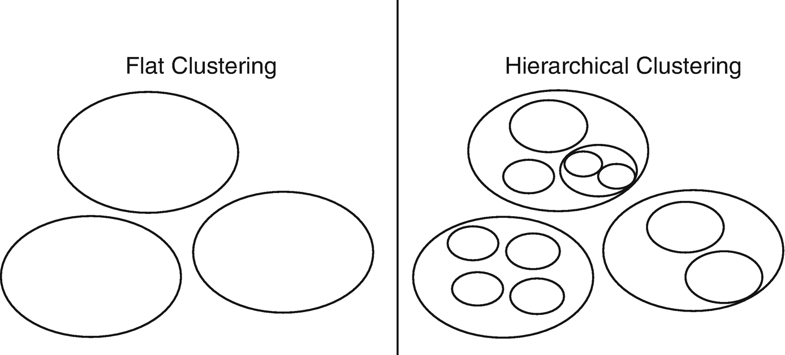
\includegraphics[scale=.4]{pic/394318_1_En_9_Fig6_HTML.png}
    \caption{扁平聚类 vs 层次聚类,核心区别是扁平聚类不体现类间关系,层次聚类反映了类的蕴含关系}
    \label{fig: cluster_taxonomy}
\end{figure}

\subsection{扁平聚类}

扁平聚类指的是得到的类,两两没有交集,所有类的并集构成了所有数据点。这一聚类的代表就是$k$-means聚类,准确说,我们先有$k$-means问题,然后才有了相关的解决这一问题的算法。$k$-means问题指的是给定数据集,寻找$k$个点使得所有点到这$k$个点的距离平方和最小。在所有解决的算法中最有名的可能就是Lloyd算法\citing{macqueen1967some}了,该算法分为以下3步。第一步,从数据集中均匀采样$k$个点作为初始化的中心点;第二步,所有点靠到离自己最近的中心点上去,形成k个类;第三步,取k个类的中心点作为新的中心点。一般来说,第二、三步会重复$t$次,因此算法的时间复杂度是$O(nkdt)$,其中$n$,$d$分别指的是待聚类的数据量和数据的维度。作为一个经典聚类算法,该算法被大量应用在自然语言处理、数据挖掘、以及其他领域中。这个算法有一些优点,首先它比较简单,易于实现。其次,它易于并行,在中等数据量下可以很好运行。但是它的一些缺点也非常瞩目,聚类的$k$值不好确定,受初始点影响大,仅能对球形数据进行聚类(如果数据非球形则聚类结果和人的直观感觉有较大出入)。

%todo: check spectral clustering
为了解决最后一个问题,谱聚类(spectral clustering)被提了出来。这一聚类算法创新性的从图分割的角度给聚类带来了新的视角,从这一视角下,一些传统上不容易被聚类的数据集也能被攻克。它的基本思想是在数据集上构建一个图,聚类问题转化为大图切割为子图的问题,好的聚类应该是,子图内部节点相似度高,子图之间相似度低。基于这一“好的”聚类的准则,人们制定了称为Ncut的切割目标函数,这一目标函数的求解可以转换为图拉普拉斯矩阵的分解问题,通过特征值分解得到新的特征,再在这一特征上聚类从而得到最终结果。
过程可总结如下:
\begin{enumerate}
    \item 根据输入的相似矩阵的生成方式构建样本的相似矩阵 $S$
    \item 根据相似矩阵 $S$ 构建邻接矩阵 $W$,构建度矩阵 $D$
    \item 计算出拉普拉斯矩阵 $L$
    \item 构建标准化后的拉普拉斯矩阵 $D^{- \frac{1}{2}}L D^{- \frac{1}{2}}$
    \item 计算 $D^{- \frac{1}{2}}L D^{- \frac{1}{2}}$最小的 $k$ 个特征值所各自对应的特征向量$f$
    \item 将各自对应的特征向量 $f$ 组成的矩阵按行标准化,最终组成 $n\times k$ 维的特征矩阵 $F$
    \item 对 $F$ 中的每一行作为一个$k$维的样本,共 $n$ 个样本,用$k$-means进行聚类,聚类数为 $k$
    \item 得到类划分
\end{enumerate}
实践中谱聚类能够很好处理$k$-means不能处理的非球形数据(比如同心圆、半月牙等),对比效果见图\ref{fig: flat_compare},这可以从谱聚类的设计准则解释,因为是做图切割,而相似度又有多种非线性的选择,所以聚类的结果就可以实现$k$-means不能做到的非线性划分($k$-means用欧式距离所以决策边界是线性的)。由于本文研究的就是$k$-means和谱聚类,所以对于他们的详细剖析见第二、三章。

\begin{figure}[h]
    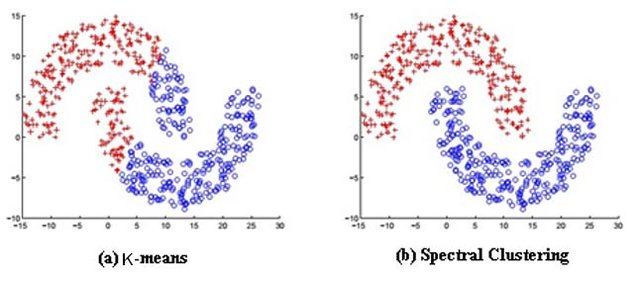
\includegraphics[scale=0.4]{pic/Comparison-between-K-Means-and-spectral-clustering_W640.jpg}
    \caption{$k$-means vs 谱聚类,可以看到谱聚类能够处理$k$-means处理不了的非球形数据}
    \label{fig: flat_compare}
\end{figure}

\subsection{层次聚类}
尽管扁平聚类的概念更简单,但我们也看到了他们的一些缺点。首先,现实世界中类和类之间是有关系的,比如说灵长类属于哺乳类,这样的蕴含关系,在扁平聚类中这样的类间关系无法体现。其次,拿$k$-means问题来说,我们需要在聚类前指定类的数目$k$,这在现实生活中未必好确定。最后,扁平聚类过程是不确定的(nondeterministic),即聚类结果有随机因素,比如Lloyd算法初始化不同结果就不同。为了解决这些问题,诞生了层次式聚类。顾名思义,层次式聚类得到的类有层级结构,可以用树状图(tree/dendrogram)来表示,如图\ref{fig: hierarchical}所示,他们也不需要指定类的数目,多数层级聚类也是确定的。这些好处的代价就是聚类速度更慢,常用的层级聚类时间复杂度至少是$O(n^2)$。

\begin{figure}[h]
    \subfloat[]{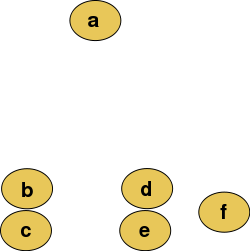
\includegraphics[scale=.5]{Clusters.svg.png}}
    \hfil
    \subfloat[]{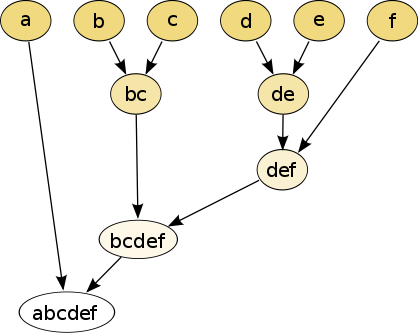
\includegraphics[scale=.4]{Hierarchical_clustering_simple_diagram.svg.png}}
    \caption{层级聚类图示。(a)示例数据集,每个字母代表一个数据点,距离越近相似度越高;(b)层级聚类后的结果,相似的类归并为一个更大的类从而形成一个二叉树,树的根节点在最下面}
    \label{fig: hierarchical}
\end{figure}

层级聚类可以自底向上做,将小的类逐渐归并得到大的类,也可以自顶向下,将大的类逐渐分割得到小的类,由此得到两种不同的聚类范式。前者称为agglomerative clustering,后者称为divisive clustering。我们先介绍前者,agglomerative clustering的一般过程如下所示
\begin{enumerate}
    \item 初始化:每个点自己作为一个类
    \item 直到所有类归并为一个类,否则
    \begin{enumerate}
        \item 找出两个最相似的类
        \item 将他们归并为一个类(父类)
    \end{enumerate}
    \item 返回类的层级结果(树)
\end{enumerate}
可以看到,这是一个贪心算法,如果有$n$个点,这个合并的过程就会持续$n-1$次,如果运气好,树的深度就是$\log_2 n$。由于树的结构,我们就可以知道类的蕴含关系,那么如何计算类和类的相似度呢?这里我们需要定义一些常用的计算方式,这些计算方式一般被称为linkage criteria,见表\ref{tab: linkage}。

\begin{table}[h]
\caption{几种常见的linkage criteria}
\begin{tabular}{cc}
\toprule
名字 & 计算方式 \\
\midrule
Maximum linkage & $\max{\{d(a,b): a \in A, b \in B\}}$ \\ 
Minimum linkage & $\min{\{d(a,b): a \in A, b \in B\}}$ \\ 
Unweighted average linkage & $\frac{1}{|A|\cdot |B|} \sum_{a \in A}\sum_{b \in B} d(a,b)$ \\
Centroid linkage & $\norm{\mu_A-\mu_B}$ \\
Ward linkage & $\frac{n_a n_b}{n_a + n_b} \norm{\mu_A-\mu_B}^2$ \\
\bottomrule
\end{tabular}
\label{tab: linkage}
\end{table}
\begin{table}[h]
\caption{几种常见的距离计算}
\begin{tabular}{cc}
\toprule
名字 & 计算方式 \\
\midrule
Euclidean distance & $\norm{a-b}_2 = \sqrt{\sum_i (a_i - b_i)^2}$ \\ 
Squared Euclidean distance & $\norm{a-b}_{2}^2 = \sum_i (a_i - b_i)^2$ \\ 
Manhattan distance & $\norm{a-b}_1 = \sum_i |a_i - b_i|$ \\
Maximum distance & $\norm{a-b}_\infty = \max_i |a_i - b_i|$ \\
\bottomrule
\end{tabular}
\label{tab: distance}
\end{table}

表格\ref{tab: linkage}中的$d$是点与点间的距离计算方式,这有很多种选择,这里挑了些常用的列在表\ref{tab: distance}中,$A,B$是两个类,$\mu_A,\mu_B$是这两个类的中心点,$n_a,n_b$是两个类中点的数目。可以看到,Maximum/Minimum/Centroid只考虑单一的点对来计算类间相似度,而Ward/Unweighted average基本考虑了全部的。值得一提的是,agglomerative clustering在聚类的过程会倾向与让大的类更大,从而导致大小不平衡的类,从这个角度讲,Minimum linkage是最差的linkage,Ward会形成差不多大小的cluster。然而在Ward中的距离计算是不可改变的(只有欧式距离),因此对于非欧的距离度量,average linkage比较合适。尽管Minimum linkage易受到噪声数据的影响,但它计算比较高效(时间复杂度是$O(n^2)$,一般的其他linkage是$O(n^2 \log n)$),因此这一linkage可以用到较大的数据量上,在非球形数据上Minimum linkage也有好的表现。

现在我们来看divisive clustering,前面说过,这是一个自顶向下的层级聚类,它需要挑选一个类,将这个类分为两个子类,并循环这个过程,直到终止条件触发(比如聚到指定数目的类)。从这个过程我们就可以看出该算法主要考虑两件事,如何挑选待分割的类以及如何分割这个类。前者一般通过某种预定义的松散度度量,比如类内最远的两个点的距离,选这个值最大的类进行分割。分割的方法一般是用扁平式聚类法,因为又包括了其他算法,divisive clustering要更复杂些。如果我们不要求划分太过细致,算法就可以在中间某层结束,如果结合Lloyd算法使用,假设我们想得到$s$个类,时间复杂度就是$O(nsdt)$,$d$和$t$分别是数据点维度和迭代次数,这样就会比agglomerative clustering快很多。有研究指出divisive clustering比 agglomerative clustering得到的层级结果质量更好\citing{karypis2000comparison},这可能是因为agglomerative是自底向上,在每次合并的时候只能看到局部的信息而不考虑全部信息,而合并过程又不可以反悔,所以divisive clustering由于是看到了全部信息做的划分,能得到更好的结果。尽管divisive clustering有这些优点,它的使用却没有agglomerative clustering频繁,可能是处理复杂情况时自底向上更符合人的习惯。

\subsection{聚类评价}
聚类评价方式分为两种,外部评价(external index)和内部评价(internal index)。前者需要有人给出的划分结果作为标准而后者不利用任何参考。我们先看外部评价,假定算法给出的类划分是$C=\{C_1, C_2,...,C_k\}$,人给出的划分是$C^* = \{C_1^*,C_2^*,...,C_s^*\}$。考虑一对数据对$(x_i,x_j)$,假设$x_i,x_j$在$C$中在同一个类里,如果算法给出的划分和人的划分是一致的,那么它们在$C^*$中也应该在同一个类里。令$\lambda_i = \{1,2,...,k\}$是数据点$x_i$的类id,即$x_i \in C_{\lambda_i}$。那么对于刚刚所说的情况可以定义一个集合$SS$来容纳这些数据对
\begin{equation*}
    SS = \{(x_i,x_j)|\lambda_i = \lambda_j,\lambda_i^* = \lambda_j^*, i<j \}
\end{equation*}
也就是说,如果数据对在$SS$集合中就意味着聚类是成功的。当然也有不成功的情况,我们定义为$SD$和$DS$。
\begin{gather*}
    SD = \{(x_i,x_j)|\lambda_i = \lambda_j,\lambda_i^* \neq \lambda_j^*, i<j \} \\
    DS = \{(x_i,x_j)|\lambda_i \neq \lambda_j,\lambda_i^* = \lambda_j^*, i<j \} \\
    DD = \{(x_i,x_j)|\lambda_i \neq \lambda_j,\lambda_i^* \neq \lambda_j^*, i<j \}
\end{gather*}
最后一行是另外一种成功的情况称为$DD$。值得注意的是,这几种情况是互不相交的,定义
\begin{equation*}
    TP = |SS|, FP = |SD|, FN = |DS|, TN = |DD|
\end{equation*}
因此有$TP+FP+FN+TN=n(n-1)/2$。基于$TP$、$FP$、$FN$和$TN$,我们可以定义以下外部评价指标($F_1$,Rand系数,Jaccard系数)
\begin{gather*}
    P = \frac{TP}{TP+FP},R = \frac{TP}{TP+FN}, F_1 = \frac{2*P*R}{P+R} \\
    \text{Rand} = \frac{TP+TN}{TP+FP+FN+TN} \\ 
    \text{Jaccard} = \frac{TP}{TP+FP+FN}
\end{gather*}
$F_1$和监督学习中的一致,Rand系数也被称为Accuracy。除去上面这些还有简单实用的Purity以及有信息论背景的NMI(Normalized Mutual Information),当类的数目比较大的时候,Purity容易比较大,而NMI缓解了此问题。
\begin{gather*}
    \text{Purity} = \frac{1}{n} \sum_i \max_j n_{ij} \\
    \text{MI}(C, C^*) = \sum_{i=1}^{|C|}\sum_{j=1}^{|C^*|}P(i, j)\log\left(\frac{P(i,j)}{P(i)P(j)}\right) \\
    H(C) = - \sum_{i=1}^{|C|}P(i)\log(P(i)) \\
    \text{NMI}(C, C^*) = \frac{\text{MI}(C, C^*)}{\text{mean}(H(C), H(C^*))}
\end{gather*}

其中,$n_{ij}=|C_i \cap C_j^*|$,$n_i = |C_i|$,$P(i) = n_i/n$,$P(i,j)=n_{ij}/n$。$P(i)$可以理解为一个数据点落在类$i$中的概率,$P(i,j)$可以理解为一个点在既在$C_i$又在$C_j^*$中的概率。MI称为互信息(mutual information),H是熵。这里所列的外部评价都是越大越好。

除了外部评价,内部评价在没有人工标注的情况下使用,比如$k$-means的目标值(objective)可以作为评价指标,该评价指标是聚类问题相关的,评价$k$-means算法用,评价其他算法慎用,还有一些聚类问题无关的评价指标,比如DB指数(Davies-Bouldin Index)
\begin{gather*}
    \text{avg} = \frac{2}{|C|(|C|-1)}\sum_{1\leq i<j \leq |C| }d(x_i,x_j) \\
    d_{cen}(C_i,C_j) = d(\mu_i,\mu_j) \\
    \text{DBI} = \frac{1}{k}\sum_{i=1}^k \max_{j \neq i} (\frac{\text{avg}(C_i)+\text{avg}(C_j)}{d_{cen}(\mu_i,\mu_j)})
\end{gather*}
其中$d$可以是表\ref{tab: distance}中的距离函数。

\section{本文的研究目标及主要贡献和创新}
在大数据下聚类,我们应该关心什么问题呢?我们应该注意那些普遍且真实的问题,所以,首先,我们应该考虑的就是聚类速度,传统聚类算法由于其自身较高的时间复杂度,在目前大数据时代越来越难以适用。其次,聚类算法的聚类质量也是一个主要问题,很多算法声称自己有好的聚类质量,并且也在一部分数据上得到了证实,但是可能换一个数据集这个算法效果就不好了,对于这种情况有时很难分析问题在哪里,这种时候我们就会希望这个算法在理论上有质量保证,比如说可以证明该算法不会比最优算法的聚类结果差多少倍。总结一下,在本文中我们将探究以下两个问题:
\begin{enumerate}
    \item 怎样聚类更加高效?
    \item 怎样聚类得出的解有理论保证?
\end{enumerate}
鉴于扁平聚类的普适性,我们将围绕$k$-means问题和谱聚类问题探究我们所提出的问题并给出我们的贡献。具体来说,我们的贡献和创新有以下几点:
\begin{enumerate}
    \item (理论\&实验贡献)对基于均匀采样加速$k$-means的算法给出了更紧的理论界,从$4(\alpha+\beta)$收缩到了$\alpha+\beta$,同时,我们证明了在温和的假设下,该算法的时间复杂度在多项式对数级别(polylogarithmic time),随后我们在实验上对理论结果进行了验证
    \item (理论贡献)将经典的$k$-means++初始化方法扩展到了带权重的$k$-means问题上并给出了证明
    \item (理论\&实验贡献)对基于Weighted kernel $k$-means的谱聚类算法给出了更紧的理论界,并给出了Weighted kernel $k$-means的MATLAB实现。
\end{enumerate}

\section{本论文的结构安排}
本文的章节结构安排如下:第一章是绪论,介绍常见聚类算法为后续探讨打下初步基础同时明确指出要研究的问题和我们的创新,第二章探讨$k$-means问题,将会分别深入分析与回答我们所提出的两个问题。第三章探讨谱聚类问题,同样加速和理论保证分别分析。第四章是结论,在总结全文的基础上给出未来可能的研究方向。
\chapter{\texorpdfstring{$k$}{k}-means聚类}
本章聚焦$k$-means问题,前面已经提到解决该问题的一个经典算法Lloyd算法,由于文献\cite{garey1982complexity,kleinberg1998microeconomic,mahajan2009planar}指出$k$-means问题是NP难的,所以该算法准确来说是一个近似算法。前面提到,该算法收到初始点影响大,所以本章将首先探讨有理论保证的$k$-means问题的算法。其次,$O(nkdt)$的时间复杂度在海量数据下也难以处理,所以接着我们会探讨如何加速。然后,我们探讨如何将这两点都覆盖,最后我们给出我们的贡献并总结本章。

\section{\texorpdfstring{$k$}{k}-means问题引入及背景知识}
% todo: add the original definition to be consistent with the weighted kernel kmeans
我们首先定义$k$-means问题,给定点$x \in \R^d$和集合$C \subseteq \R^d$,$d$是数据的维度,我们可以定义该点到集合的距离
\begin{equation*}
d(x,C) = \min\limits_{c \in C}\norm{x - c}
\end{equation*}
给定$n$个点的数据集$\mathcal{X} \subseteq \R^d$和集合$C \subseteq \R^d$,我们可以定义如下目标函数
\begin{equation*}
\varphi(\mathcal{X},C) = \sum_{x \in \mathcal{X}}d^2 (x,C)
\end{equation*}
我们的目标是在给定$n$个点$\mathcal{X}$情况下找到大小为$k$的集合$C_{\text{OPT}_k}^\mathcal{X}$使得该目标函数最小,即
\begin{equation*}
C_{\text{OPT}_k}^\mathcal{X} = \argmin\limits_{ \substack{C \subseteq \R^d \\ |C| = k} }\varphi(\mathcal{X},C)
\end{equation*}
上文谈到解的质量,这里给出如下定义用于定量评价解的质量。
\begin{definition}[$k$-means问题解的质量]
    \label{def: k-means_quality}
    一个算法 $\mathcal{A}$被称为$k$-means问题的一个$\alpha$近似算法如果存在一个数字$\alpha \geq 1$使得
    \begin{equation*}
        \varphi(\mathcal{X},C) \leq \alpha \varphi(\mathcal{X},C_{\text{OPT}_k}^{\mathcal{X}})
    \end{equation*}
    成立,此时称解$C$为
一个$\alpha$近似解,这里$\alpha$称为近似系数。
\end{definition}
从该定义可以看出, $\alpha$越小解质量越好,越接近最优解。
\section{改进\texorpdfstring{$k$}{k}-means的聚类质量}

选择好的初始化方法(seeding) 是提供质量保证的一条路
线, 在 Lloyd 算法中传统初始化方法一般是均匀不放回的抓取$k$个点,这不是一个好的初始化方法, 由于 Lloyd 算法对初始
点很敏感\citing{cao2009initialization},这种方法为了取得好的效果经常需要多次初始
化取最好的, 除去花费不少时间此种方法没有理论上的保证,
而 David等人\citing{arthur2007k}则在这一方向上做出了巨大的贡献。

首先, 从直觉上想,当初始化的点聚在一起的时候该初始
化就不是一个好的初始化,因此一种容易相到的就是每次新选
择的点都应离已经选择的点尽可能远,但是如果直接选择最远
的点的话就可能是异常点,为此可以这样改进该算法,每一个
点以一个概率被选中,而该概率与该点到已选择到的点的距离成正比,由此便得到了 $k$-means++算法\citing{arthur2007k},算法详细描述如
算法\ref{alg:Kmeans++ seeding}

\begin{algorithm}
    \caption{$k$-means++ seeding}\label{alg:Kmeans++ seeding}
    \KwIn{数据集 $\mathcal{X}$,类数目$k$}
    \KwOut{$k$个点 $C$}
    $c_1 \gets $ 从$\mathcal{X}$中均匀采样一个点 \\
    $C \gets \{c_1\}$ \\
    \For{$i = 2,3, \ldots k$}{
        \For{$x \in \mathcal{X}$}{
            % we can calculate a small set of p instead of whole p(x)
            $p(x) \gets \text{d}(x,C)^2/\sum_{x' \in \mathcal{X}} \text{d}(x',C)^2$
        }
        $x \gets$ 从$\mathcal{X}$中依分布$p(x)$采样一个点 \\
        $C \gets C\cup\{x\}$
    }
    \textbf{返回} $C$
\end{algorithm}
该算法的时间复杂度为$O(nkd)$,实验验证在使用 $k$-means++ seeding 后 Lloyd 算法能更快收敛。另外, 对于 $k$-means++以下定理成立
\begin{theorem}[$k$-means++解的质量]
    对于任意数据集$\mathcal{X}$
    \begin{equation}
    \E[\varphi(\mathcal{X},C)] \leq 8(\ln k + 2) \varphi(\mathcal{X},C_{\text{OPT}_k}^{\mathcal{X}})
    \end{equation}
    其中$C$算法\ref{alg:Kmeans++ seeding}返回的结果
\end{theorem}
可以看出即使以初始化的$k$个点作为最后的解,解的平均
质量已经能够达到$O(\log k)$,后续 Lloyd 算法的步骤只会让解
更好。

那么,能否获得常数近似的解呢? 设想现在已经有一个解
的集合 $T \subset \mathcal{X}$,为了在$T$基础上得到更好的解,可以采取以下
策略,将点$t\in T$替换为$T' \in \mathcal{X}-T$得到 $T'$,如果$T'$的解质量更
好,则用$T'$替换$T$,重复该步骤直到解质量不再变化。算法描
述见算法\ref{alg:p-swap},
\begin{algorithm}
    \caption{启发式本地搜索算法(p-swap)}\label{alg:p-swap}
    \KwIn{数据集 $\mathcal{X}$,类数目$k$}
    \KwOut{$k$个点 $T$}
    $T \gets $ 从$\mathcal{X}$中随机选$k$个点 \\
    \While{$ \exists t \in T, t' \in \mathcal{X}-T$ 使得 $\varphi(\mathcal{X},T-\{t\}+\{t'\})< \varphi(\mathcal{X},T)$}{
        $T \gets T-\{t\}+\{t'\}$
    }
    \textbf{返回} $T$
\end{algorithm}
在实际应用中这个替换会持续很久,不过,通过对文献
\cite{arya2004local}和文献\cite{charikar1999improved}的结果进行拓展,该算法可以在多项式时间(polynomial time)内收敛。 首先,对于任意1次替换不能再减少$k$-means 目标函数值的解称其为1-stable 的解。基于此, Arya等人\citing{arya2004local}和Kanungo等人\citing{kanungo2004local}对解的质量给出了如下的理论结果。
\begin{theorem}[1-stable的解的质量]
    令 $O \subset \mathcal{X}$,且是所有大小为$k$的$\mathcal{X}$的子集里能取得最小$k$-means 目标函数值的那个解,令$T$是 1-stable 的解,则有
    \begin{equation}
        \varphi(\mathcal{X},T) \leq 25 \varphi(\mathcal{X},O)
    \end{equation}
\end{theorem}
值得注意的是$O$并不是$C_{\text{OPT}_k}^{\mathcal{X}}$,通过简单的推论,得知近似系数是50(乘以2)。那对于任意p-stable 的解,近似系数是多少呢?Kanungo 等人\citing{kanungo2004local}对算法\ref{alg:p-swap}的分析做了推广得到以下结论。
\begin{theorem}[p-stable的解的质量]
    令 $O \subset \mathcal{X}$,且是所有大小为$k$的$\mathcal{X}$的子集里能取得最小$k$-means 目标函数值的那个解,令$T$是 p-stable 的解,则有
    \begin{equation}
        \varphi(\mathcal{X},T) \leq (3+\frac{2}{p})^2 \varphi(\mathcal{X},O)
    \end{equation}
\end{theorem}
可见对于充分大的 p,系数是 18。实验表明算法\ref{alg:p-swap}收敛相对于 Lloyd 算法收敛慢,但是该算法能够避免陷入局部极小值。
所以,实际使用时会和 Lloyd 算法混合使用,即先用一次替换再进行 Lloyd 算法的 2、 3 步,这样的混合算法在实际中有很好
的表现,文献\cite{kanungo2004local}对此做了验证。

$k$-means++虽然实用,但是近似系数只有$O(\log k)$,本地搜索算法虽然有常数的近似系数,但是不实用,时间复杂度有
$O(n^3)$,能否将这两种算法结合起来得到一个既有常数近似又快速实用的算法呢? Silvio等人\citing{pmlr-v97-lattanzi19a}便带来了一个这样的算法,算法描述见算法\ref{alg: k++_p-swap}。
\begin{algorithm}
    \caption{$k$-means++和本地搜索算法的混合算法($k$-means++\&swap)}\label{alg: k++_p-swap}
    \KwIn{数据集 $\mathcal{X}$,类数目$k$}
    \KwOut{$k$个点 $C$}
    $C \gets $ 将$(\mathcal{X},k)$应用于算法\ref{alg:Kmeans++ seeding} \\
    \For{i = 2,3,...,$z$}{
        $C = \text{LocalSearch++}(\mathcal{X},C)$
    }
    \textbf{返回} $C$
\end{algorithm}
\begin{algorithm}
    \caption{LocalSearch++算法}\label{alg: local_search++}
    \KwIn{数据集$\mathcal{X}$,解集$C$}
    \KwOut{$k$个点$C$}
    $p \gets$ 以 $d^2 (p,C)/ \sum_{q \in \mathcal{X}}d^2 (q,C)$的概率采样$p$ \\
    \If{$ \exists q \in C$ 使得 $\varphi(\mathcal{X},C-\{q\}+\{p\})<\varphi(\mathcal{X},C)$}{
        $q \gets$ 选择一个$q$使得$\varphi(\mathcal{X},C-\{q\}+\{p\})$最小 \\
        $C = C-\{q\}+\{p\}$
    }
    \textbf{返回} $C$
\end{algorithm}
\begin{theorem}[$k$-means++和本地搜索的混合算法的解的质量]
    \label{thrm: k++_p-swap}
     令$C$是算法\ref{alg: k++_p-swap}的解,且$z \geq 100000 k \log\log k$,则有
     \begin{equation}
         \E[\varphi(\mathcal{X},C)] \in O(\varphi(\mathcal{X},C_{\text{OPT}_k}^{\mathcal{X}}))
     \end{equation}
\end{theorem}
算法\ref{alg: k++_p-swap}的理论保证由定理\ref{thrm: k++_p-swap}给出,该定理说明只要迭代大
概$O(k)$次LocalSearch++,解的近似系数就能达到常数,此时算法\ref{alg: k++_p-swap}的时间复杂度是$O(ndk^2 \log\log k)$。实验表明在不使用Lloyd 算法后续迭代的情况下,混合的算法\ref{alg: k++_p-swap}比$k$-means++好8-
35\%,而使用 Lloyd 迭代 10 次后,依然能比$k$-means++好1-18\%

尽管$k$-means++在线性时间里能得到不错的解,但是其序列化属性使得该算法无法并行,因此在大数据下难以适用, $k$-means\(\vert \vert\)采样便是为了解决这个问题而被提出的,它的想法是基于已经挑选出的点集,下一次不止挑选一个点而是挑选一个集合,其期望大小为$l$,将若干次挑选出来的集合汇总之后再在其上做聚类即可,采样算法详细描述见算法\ref{alg: kmeans||_sample},对于算法\ref{alg: kmeans||_sample}有如下理论保证。
\begin{theorem}[$k$-means\(\vert \vert\)采样理论保证1]
    \label{theo: kmeans||_performance_1}
    令$S$是算法\ref{alg: kmeans||_sample} $t$次迭代后返回的结果,有
    \begin{equation}
    \E[\varphi(\mathcal{X},S)] \leq (\frac{1+\alpha}{2})^t \xi + \frac{16}{1-\alpha}\varphi(\mathcal{X},C_{\text{OPT}_k}^{\mathcal{X}})
    \end{equation}
    其中$\alpha=exp(-(1-e^{-l/(2k)})) \approx e^{-\frac{l}{2k}}$
\end{theorem}
\begin{algorithm}
    \caption{$k$-means\(\vert \vert\)采样算法}\label{alg: kmeans||_sample}
    \KwIn{数据集$\mathcal{X}$,每一轮期望采样数$l$}
    \KwOut{采样集$S$}
    $S \gets$ 在$\mathcal{X}$中均匀采样一个点 \\
    $\xi \gets \varphi(\mathcal{X},S)$ \\
    \For{i = 1,2,...,$\log \xi$}{
        $C' \gets \emptyset$ \\
        \For{$x \in \mathcal{X}$}{
            以概率 $\min(1,\frac{ld^2 (x,S)}{\varphi(\mathcal{X},S)})$将$x$加入$C'$中
        }
        $S \gets  S \cup C'$
    }
    \textbf{返回} $S$
\end{algorithm}
上述定理说明算法\ref{alg: kmeans||_sample}经过$O(\log \xi)$次迭代之后,只要$l$足够大,所有点到挑选出来的$S$个点的距离和已经降到了$O(\varphi(\mathcal{X},C_{\text{OPT}_k}^\mathcal{X}))$,也就是说和最优的距离和已经在一个级别了。 接着在$S$上聚类便可
以得到$k$-means的解, 在这里为了使解有理论上的保证, 需要对$S$上的点加权重,首先定义如下带权$k$-means问题。
\begin{definition}[带权$k$-means问题]
    \label{def: weighted_kmeans}
    给定集合 $\mathcal{X} \subseteq \R^d$ 和每一个$x \in \mathcal{X}$ 的权重 $w_i$, 找到一个大小为$k$的集合 $C \subseteq \R^d$ 使得下述目标函数能最小
    \begin{equation}
        \psi(\mathcal{X},C) = \sum_{x_i \in \mathcal{X}}w_i d^2 (x_i,C)
    \end{equation}
\end{definition}
接着在带权重的$S$上聚类得到算法\ref{alg: kmeans||_seeding},
\begin{algorithm}
    \caption{$k$-means\(\vert \vert\) seeding算法}\label{alg: kmeans||_seeding}
    \KwIn{数据集$\mathcal{X}$,每一轮期望采样数$l$,聚类数$k$}
    \KwOut{$k$个点$C$}
    $S \gets$ 将 $(\mathcal{X},l)$ 应用于算法\ref{alg: kmeans||_sample} \\
    对点$s_i \in S$,令$w_i$是$\mathcal{X}$中离$s_i$最近的点的数目 \\
    $C \gets$ 令$w_i$是$s_i$的权重,在带权的$S$上运行一个$\alpha$近似算法 \\
    \textbf{返回} $C$
\end{algorithm}
可以证明,如果使用的是$\alpha$近似算法,那算法\ref{alg: kmeans||_seeding}输出的$k$
个点便是原$k$-means问题的一个$O(\alpha)$近似解。 在实践中发现当$l$较大时,往往不需要$\log \xi$次迭代, O. Bachem\cite{bachem2017distributed}的分析证实
了这一点,令迭代次数为$t$, 则有下述定理。
\begin{theorem}[$k$-means\(\vert \vert\)采样理论保证2]
    令$k \in \N$,$t \in \N$,且$l \geq k$,令$\mathcal{X} \subseteq \R^d$且$S$是算法\ref{alg: kmeans||_sample}返回的结果,则
    \begin{equation}
    \E[\varphi(\mathcal{X},S)] \leq 2(\frac{k}{el})^t \text{Var}(\mathcal{X}) + 26\varphi(\mathcal{X},C_{\text{OPT}_k}^{\mathcal{X}})
    \end{equation}
\end{theorem}
该定理同定理\ref{theo: kmeans||_performance_1}关键区别是只要$l$足够大,指数衰减的速度可以任意快,而定理\ref{theo: kmeans||_performance_1}的衰减速度最多是1/2。虽然$k$-means\(\vert \vert\)时间复杂度是$O(nld \log n)$(如果$t$次迭代则是$O(nltd)$),比Lloyd算法高,但是它易于并行,因此在能够并行的情况下很多经典大数据处理框架都采用了该算法比如Spark\citing{zaharia2010spark,zaharia2016apache}。

除了改善$k$-means++的序列化属性来加速seeding外,还可以用其他方法加速。通过分析即可知道在$k$-means++方法中最费时间的是找到计算概率所需要的分母,有没有在不知道分母的情况下近似采样分布的方法呢?有,该算法便是MH算法\citing{hastings1970monte},该算法属于MCMC方法,其基本想法是构建一个马尔可夫链使得其平稳分布(stationary distribution)等于要采样的分布,这样就可以通过随机游走的方式来近似采样,基于MCMC来近似$k$-means++
的方法称为K-M$\text{C}^2$\citing{bachem2016approximate}, Bachem等人通过对数据集生成的分
布做出假设使得基于马尔科夫链随机游走的时间复杂度被限制在次线性时间(sub-linear time)内,从而让K-M$\text{C}^2$在$O(k^3 d \log^2 n \log k)$的时间复
杂度下获得了$k$-means++的近似系数。K-M$\text{C}^2$算法见算法\ref{alg:K-MC^2 seeding},算法中$Unif(0,1)$指的是0-1中均匀采样的一个数。为了让游走能尽快收敛到平稳分布,我们定义如下两个数据相关的指标:
\begin{equation}
\zeta(\mathcal{X}) = \max\limits_{x \in \mathcal{X}}\frac{d(x,\mu(\mathcal{X}))^2}{\sum_{x' \in \mathcal{X}}d(x',\mu(\mathcal{X}))^2}, \eta(\mathcal{X}) = \frac{\varphi(\mathcal{X},C_{\text{OPT}_1}^{\mathcal{X}})}{\varphi(\mathcal{X},C_{\text{OPT}_k}^{\mathcal{X}})}
\end{equation}
假定数据是从生成数据的分布$F$中独立同分布的采样出来的,且该分布满足以下两个假设,如果满足这些假设的话$\zeta(\mathcal{X})$和
$\eta(\mathcal{X})$就可以被限定住,游走就能很快收敛到平稳分布

\textbf{假设1} 分布$F$的尾部是指数衰减的,即$\exists c,t $使得$P[d(x,\mu(F))>a]\leq ce^{-at}$,其中$x\sim F$ 

\textbf{假设2} $F$在一个球面上的最大和最小概率密度被一个常数限制

如果满足假设1和2分别有以下推论和定理。
\begin{corollary}
    \label{cor: zeta_x}
    如果假设1成立,有$\zeta(\mathcal{X}) = O(\log^2 n)$
\end{corollary}
\begin{corollary}
    \label{cor: eta_x}
    如果假设2成立,有$\eta(\mathcal{X}) = O(k)$
\end{corollary}
\begin{theorem}
    \label{theo:Kmc^2 performance}
    在假设1和2成立的情况下,令$C$为算法\ref{alg:K-MC^2 seeding}的返回结果,有
    \begin{equation}
    \E[\varphi(\mathcal{X},C)]\leq O(logk)\varphi(\mathcal{X},C_{\text{OPT}_k}^{\mathcal{X}}))
    \end{equation}
    此时,$m = O(k\log^2 n\log k)$,算法时间复杂度为$O(k^3 d \log^2 n \log k)$
\end{theorem}
\begin{algorithm}[ht]
    \caption{K-M$\text{C}^2$ seeding}\label{alg:K-MC^2 seeding}
    \KwIn{数据集$\mathcal{X}$,游走次数$m$,类数目$k$}
    \KwOut{$k$个点$C$}
    $c_1 \gets $ 从$\mathcal{X}$中均匀采样一个点 \\
    $C \gets \{c_1\}$ \\
    \For{$i = 2,3, \ldots k$}{
        $x \gets $ 从$\mathcal{X}$中均匀采样一个点 \\
        $d_x \gets \text{d}(x,C)^2$ \\
        \For{$j = 2,3, \ldots m$}{
            $y \gets $ 从$\mathcal{X}$中均匀采样一个点 \\
            $d_y \gets \text{d}(y,C)^2$ \\
            \If{$\frac{d_y}{d_x}$ > Unif(0,1)}{
                $x \gets y, d_x \gets d_y$ \\
            }
        }
        $C \gets C\cup\{x\}$ \\
    }
    \textbf{返回} $C$ % can add comment like this \Comment{The gcd is b}
\end{algorithm}
该方法在次线性时间里完成了$O(\log k)$的近似,因此在数据较大且不能很好并行的情况下应该优先使用该算法。然而,在实践中该方法有以下缺点:
\begin{enumerate}
    \item 如果存在小的类且该类离其他类比较远,那由于均匀选择的点很难落在小的类里,这样该方法就会产生较大的距离和
    \item 不少现实中的数据不满足上述假设,比如经常能观测到重尾分布(heavy tailed distributions)的数据
    \item 验证上述假设是困难的,比如计算$\zeta(\mathcal{X})$需要对数据进行两次遍历,计算$\eta(\mathcal{X})$更是NP难的
    \item 定理\ref{theo:Kmc^2 performance}并没有描述游走次数$m$和算法解的质量之间的权衡,只有选择特定的游走次数才有效,因此,如果假设不
成立,就得不到任何理论上的保证
\end{enumerate}
因此,需要提出新的算法解决这些问题。

AFK-M$\text{C}^2$\citing{bachem2016fast}通过使用提议分布(proposal distribution)很好的解决了这些问题,首先通过该提议分布,$\zeta(\mathcal{X})$的假设得以废弃;第二,一种新的理论分析使得在不假设$\eta(\mathcal{X})$的情况下也能获得解的质量的理论保证;最后, 新的结果表明了游走次数$m$和算法质量之间的权衡。 AFK-M$\text{C}^2$描述在算法\ref{alg:AFK-MC^2 seeding}中。可以看出点的选择依赖提议分布$q$, 因此小的类也能被选到点,从而解决了K-M$\text{C}^2$方法中的问题1。对于AFK-M$\text{C}^2$,有如下定理
\begin{theorem}[AFK-M$\text{C}^2$理论结果]
    \label{theo:AFKmc^2 performance}
    令$\epsilon \in (0,1)$ 且$k \in \N$。令数据集$\mathcal{X} \subseteq \R^d$,$|\mathcal{X}| = n$,$C$是算法\ref{alg:AFK-MC^2 seeding}的输出,$m = 1+\frac{8}{\epsilon}log \frac{4k}{\epsilon}$,则
    \begin{equation}
    \E[\varphi(\mathcal{X},C)]\leq 8(\log_{2}k+2)\varphi(\mathcal{X},C_{\text{OPT}_k}^{\mathcal{X}}) + \epsilon\text{Var}(\mathcal{X})
    \end{equation}
\end{theorem}
\begin{algorithm}
    \SetNoFillComment
    \caption{AFK-M$\text{C}^2$ seeding}\label{alg:AFK-MC^2 seeding}
    \KwIn{数据集$\mathcal{X}$, 游走次数$m$,类数目$k$}
    \KwOut{$k$个点$C$}
    \tcc{预处理}
    $c_1 \gets $ 从$\mathcal{X}$中均匀采样一个点 \\
    \For{$x \in \mathcal{X}$}{
        $q(x) \gets \frac{1}{2}\text{d}(x,c_1)^2/\sum_{x' \in \mathcal{X}} \text{d}(x',c_1)^2 + \frac{1}{2n}$
    }
    \tcc{主循环}
    $C \gets \{c_1\}$ \\
    \For{$i = 2,3, \ldots k$}{
        $x \gets $ 依分布$q$从$\mathcal{X}$中采样一个点 \\ 
        $d_x \gets \text{d}(x,C)^2$ \\
        \For{$j = 2,3, \ldots m$}{
            $y \gets $ 依分布$q$从$\mathcal{X}$中采样一个点 \\
            $d_y \gets \text{d}(y,C)^2$ \\
            \If{$\frac{d_y q(x)}{d_x q(y)}$ $>$ \text{Unif(0,1)}}{
                $x \gets y, d_x \gets d_y$
            }
        }
        $C \gets C\cup\{x\}$
    }
    \textbf{返回} $C$
\end{algorithm}
其中$\text{Var}(\mathcal{X})=\sum_{x \in  \mathcal{X}}d(x,\mu(\mathcal{X}))^2$,容易分析得,算法中预处理花费时间为$O(nd)$,主要循环花费时间为$O(\frac{1}{\epsilon}k^2 d\log \frac{k}{\epsilon})$。虽然预处理需要花费线性的时间,时间复杂度比K-M$\text{C}^2$高,但是我们有以下理由认为实践中该步骤问题不会很大
\begin{enumerate}
    \item 对所有数据只需遍历一次
    \item 该步骤很容易并行
    \item 从定理可以看到,预处理后游走的步数从$\log^2 n$变到了常数
\end{enumerate}
因此该算法和K-M$\text{C}^2$一样,在实际中有良好的适用性,另外,定理\ref{theo:AFKmc^2 performance}良好的揭示游走次数同聚类质量间的联系,可以看到随着$\epsilon$的减小,游走步数$m$逐渐增大,聚类质量逐渐向$k$-means++的质量靠拢。同时,如果对数据的假设$\eta(\mathcal{X})$满足的话,我们可以得到下述推论。
\begin{corollary}
    令$k \in \N$,数据集$\mathcal{X} \subseteq \R^d$,$|\mathcal{X}| = n$,且满足$\beta(\mathcal{X}) = O(k)$,$C$是算法\ref{alg:AFK-MC^2 seeding}的输出,$m = O(k\log k)$,则
    \begin{equation}
    \E[\varphi(\mathcal{X},C)]\leq 8(\log_{2}k+3)\varphi(\mathcal{X},C_{\text{OPT}_k}^{\mathcal{X}})
    \end{equation}
\end{corollary}
此时,算法中预处理花费时间为$O(nd)$,主要循环花费时间为$O(k^3 d \log k)$。实验结果表明,对于大数据集,在0到1\%的相对误差下,AFK-M$\text{C}^2$算法要比$k$-means++快200到1000倍。

除去前述的假设1和2,也有些其他假设值得注意。 Ben-David\citing{ben2004framework}通过引入聚类描述方案(clustering description scheme)
并在其上添加性质,获得了常数近似系数的解,且该算法的时间复杂度是常数。文献\cite{ben2004framework}的主要假设叫做$\alpha$-m-covering,
它要求对领域集合(domain set)中的任何子集$S$,通过应用聚类描述方案到$S$的一个$l$元组上,$S$的最优聚类能被$\alpha$近似。

至此, 本节梳理了一些有理论保证的算法同时在实验上对他们进行了比较,值得注意的是文献\cite{awasthi2015hardness,lee2017improved}指出 $k$-means问题是APX难的,多项式时间内不存在近似系数小于1.0013 的解,目前最好的近似系数是 6.357\citing{ahmadian2017better}。不过,近似系数越小的算法越慢,越难以实用。另外,$k$-means问题可以构造PTAS(Polynomial Time Approximation Scheme)的解,即在多项式时间内取得1+$\epsilon$的近似,相关文献有\cite{feldman2007ptas,jaiswal2014simple,friggstad2019local}。
\section{更快得到\texorpdfstring{$k$}{k}-means的解}
本节分析如何加速$k$-means的求解,目前有两种方法加速,一种是减少数据量,还有一种利用三角不等式。

加速聚类的一个自然的想法是将大数据浓缩,得到小数据,
在小数据上聚类。用小数据上的解作为大数据上的解。由于用于减少数据量的采样方法有很多,这是一个框架性算法,算法列在\ref{alg: reduce_k-means}中。
\begin{algorithm}
    \caption{基于减少数据量的$k$-means算法}\label{alg: reduce_k-means}
    \KwIn{数据集$\mathcal{X}$,类数目$k$,聚类算法$\mathcal{A}_c$,采样算法$\mathcal{A}_s$,采样数$m$}
    \KwOut{$k$个点$C$}
    $S \gets$ $\mathcal{A}_s(\mathcal{X},m)$ \\
    $C \gets$ $\mathcal{A}_c(S,k)$ \\
    \textbf{返回} $C$
\end{algorithm}
在上一节提到的理论保证算法都可以扩展后当$\mathcal{A}_s$,比如将$k$-means++、K-M$\text{C}^2$、AF-KM$\text{C}^2$的seeding数目从$k$增加到$m$,使用$k$-means\(\vert \vert\)采样,将局部搜索的返回$k$个点增加到返回$m$个点,以及经典的均匀采样。虽然理论保证的算法可以扩展为采样算法,但是他们主要目的还是提供理论保证,而有一个技术是专门压缩数据量的,称为Coreset。

通俗来讲,Coreset指的是一些特殊的采样点(可能带权重),给定任意$k$个点,这些采样点到这$k$个点的距离平方和都能够近似所有点到这$k$个点的距离平方和,定义见\ref{def: coreset}。
\begin{definition}[常规Coreset]
    \label{def: coreset}
    带权重集合$S$是数据集$\mathcal{X}$一个$\epsilon$-Coreset,如果对任意集合$C \subset \R^d$,$|C|=k$满足
    \begin{equation*}
        |\varphi(\mathcal{X},C) - \psi (S,C)| \leq \epsilon \varphi(\mathcal{X},C)
    \end{equation*}
\end{definition}
这是一个非常强的定义,因为它要求对所有$C$都要符合定义的约束,所以符合定义\ref{def: coreset}的Coreset也被称为Strong Coreset。对于Strong Coreset,它的一个良好的性质是采样点上的最优距离平方和就可以近似所有点上的最优距离平方和。
\begin{corollary}[Coreset性质1]
    \label{cor: coreset_property1}
    令$\epsilon \in (0, \frac{1}{3})$,$S$是数据集$\mathcal{X}$的一个$\epsilon$-Coreset,则有
    \begin{equation*}
        \varphi(\mathcal{X},C_{\text{OPT}_k}^S) \leq (1+3\epsilon) \varphi(\mathcal{X},C_{\text{OPT}_k}^{\mathcal{X}})
    \end{equation*}
\end{corollary}
目前效果很好的$\epsilon$-Coreset基于重要性采样(importance sampling),算法见文献\cite{bachem2018sampling}中算法9,其采样数目为$O(\frac{k\log k}{\epsilon^2}(dk\log k+\log\frac{1}{\delta}))$,时间复杂度为$O(ndk\log\frac{1}{\delta})$,对于采样点来说近似系数是$1+O(\epsilon)$。该方法的近似系数非常好而花费的时间又是线性的,可以说是目前$k$-means问题中相当好的算法。

虽然常规的Coreset如$\epsilon$-Coreset效果好,但是花费的时间还是稍微有点多,Lightweight Coreset\citing{bachem2017scalable}即是牺牲了一部分聚类的质量来换取速度的提升, 具体来说Lightweight Coreset指的是满足定义\ref{def: lightweight_coreset}的带权点集。
\begin{definition}[Lightweight Coreset]
    \label{def: lightweight_coreset}
    令$\epsilon > 0$,$k \in \N$,$\mathcal{X} \subset \R^d$,它中心点是$\mu(\mathcal{X})$,如果对任意$Q \in \{Q'| Q' \subset \R^d, |Q'| \leq k\}$有
    \begin{equation*}
        |\varphi(\mathcal{X},Q) - \psi(S,Q)| \leq \frac{\epsilon}{2}\varphi(\mathcal{X},Q) + \frac{\epsilon}{2}\varphi(\mathcal{X},\mu(\mathcal{X}))
    \end{equation*}
    则称$S$是一个$(\epsilon,k)$-Lightweight Coreset
\end{definition}
效仿推论\ref{cor: coreset_property1},易得其有以下近似系数的推论。
\begin{corollary}[Lightweight Coreset性质]
    如果$S$是一个$(\epsilon,k)$-Lightweight Coreset,有
    \begin{equation*}
        \varphi(\mathcal{X},C_{\text{OPT}_k}^S) \leq \varphi(\mathcal{X},C_{\text{OPT}_k}^{\mathcal{X}}) + 4\epsilon\varphi(\mathcal{X},\mu(\mathcal{X}))
    \end{equation*}
\end{corollary}
构造该Coreset的算法见算法\ref{alg: Lightweight coreset},该算法有如下理论保证
\begin{algorithm}
    \caption{Lightweight coreset}\label{alg: Lightweight coreset}
    \KwIn{数据集$\mathcal{X}$, 采样点数目$m$}
    \KwOut{$m$个点 $S$}
    $\mu \gets$ 计算$\mathcal{X}$的均值 \\
    \For{$x \in \mathcal{X}$}{
        $q(x) \gets \frac{1}{2}\text{d}(x,\mu)^2/\sum_{x' \in \mathcal{X}} \text{d}(x',\mu)^2 + \frac{1}{2n}$
    }
    $S \gets $ 依分布$q$从$\mathcal{X}$中采样$m$个点且每个点$x$的权重是$\frac{1}{m.q(x)}$ \\
    \textbf{返回} $S$
\end{algorithm}
\begin{theorem}[Lightweight Coreset理论保证]
    \label{theo: lightweight_coreset}
    令$\epsilon>0$,$\delta>0$,且$k\in \N$。令$\mathcal{X}$是$\R^d$中的数据点,令$S$是算法\ref{alg: Lightweight coreset}的输出。其中采样数
    \begin{equation*}
        m \geq c\frac{dk\log k + \log(1/\delta)}{\epsilon^2}
    \end{equation*}
    其中$c$是一个常数。这样就可以至少1-$\delta$的概率使得集合$S$是一个$(\epsilon,k)$-Lightweight Coreset。
\end{theorem}
该定理说明只要采样常数个点(与$n$无关),算法就可以在$O(nd)$的时间复杂度里取得好的聚类结果(如果$\varphi(\mathcal{X},C_{\text{OPT}_1}^{\mathcal{X}})/\varphi(\mathcal{X},C_{\text{OPT}_k}^{\mathcal{X}})$不大的话)。特别的,如果前述假设2满足的话,对于采样点来说近似系数就变为了$1+O(k\epsilon)$。%remark: 对于采样点来说近似系数就变为了$1+O(k\epsilon)$ 说法不严谨,\phi(X,C_{opt_k}^S)是$1+O(k\epsilon)$ 不是\phi(X,S)

构造 Coreset 的方法除了这里提到的,还有很多, 比如还
可以用$k$-means++构造Coreset\citing{ackermann2012streamkm++},Coreset作为一个经典的数
据压缩范式还被用于其他机器学习问题中,比如PCA, NNMF(Non Negative Matrix Factorization)等,文献\cite{bachem2017practical}和\cite{feldman2013turning}是很好的参考资料。

除了减少数据量,基于三角不等式也可以加速,由于本论文工作和该方向重合度不高,感兴趣的读者可参考文献\cite{ding2015yinyang,elkan2003using,drake2012accelerated,newling2018novel}。
\section{加速\texorpdfstring{$k$}{k}-means且有理论保证}
很多时候我们希望算法既有理论保证也要速度快,本节我们将介绍这类算法。算法的基本思想是用前文减少数据量的方法减少数据,然后在少量数据上运行有理论保证的算法,接着证明这个解对于全部点也是有保证的。
\begin{algorithm}
    \caption{基于均匀不放回采样的$k$-means算法}\label{alg: uniform_k-means}
    \KwIn{数据集$\mathcal{X}$,类数目$k$,采样数$s$}
    \KwOut{$k$个点$C$}
    $S \gets$ 从$\mathcal{X}$中均匀采样$s$个点\\
    $C \gets$ 在$S$上运行一个$\alpha$近似算法\\
    \textbf{返回} $C$
\end{algorithm}
一种简单且有理论保证的减少数据量的方式是均匀采样\citing{Mohan:2017:BNA:3172077.3172235},算法详
细描述见算法\ref{alg: uniform_k-means},可以证明该方法有如下理论保证。
\begin{theorem}[均匀不放回采样的解的质量]
    \label{theo: uniform_k-means}
    令 $0 < \delta <1/2$, $\alpha \geq 1$, $\beta >0$是近似的参数。 令 C 是由算法 \ref{alg: uniform_k-means}返回的点. 假设我们均匀不放回的采样s个点,使得,
    \begin{equation*}
    s \geq \ln(\frac{1}{\delta})(1+\frac{1}{n})/(\frac{\beta^2 m^2}{2\Delta^2 \alpha^2}+\frac{\ln(1/\delta)}{n})
    \end{equation*}
    则,我们有
    \begin{equation*}
    \varphi(\mathcal{X},C) \leq 4(\alpha + \beta)\varphi(\mathcal{X},C_{\text{OPT}_k}^{\mathcal{X}})
    \end{equation*}
    以至少 $1-2\delta$的概率, 其中$\Delta = \max\limits_{i,j}\norm{x_i - x_j}^2$是数据直径的平方, $m = \varphi(\mathcal{X},C_{\text{OPT}_k}^{\mathcal{X}})/n$是点到其对应的中心点的距离的平均值。
\end{theorem}
该方法优点是简单,但是该方法的采样点数目由数据点的直径决定,如果直径较大,该方法便会失去实用价值。类似的还有基于均匀放回采样的算法\citing{czumaj2004sublinear}。

为了解决直径的问题,我们可以使用其他有理论保证的采样算法替换算法\ref{alg: reduce_k-means}中的算法$\mathcal{A}_s$,不过替换之后为了使最终解有理论保证,需要修改算法\ref{alg: reduce_k-means},即给采样点带上权重,权重是采样点对应的类的大小,修改后的算法见\ref{alg: reduce_k-means2}。
\begin{algorithm}
    \caption{基于减少数据量的$k$-means算法2}\label{alg: reduce_k-means2}
    \KwIn{数据集$\mathcal{X}$,类数目$k$,聚类算法$\mathcal{A}_c$,有理论保证的采样算法$\mathcal{A}_s$,采样数$s$}
    \KwOut{$k$个点$C$}
    $S \gets$ $\mathcal{A}_s(\mathcal{X},s)$ \\
    对点$s_i \in S$,令$w_i$是$\mathcal{X}$中离$s_i$最近的点的数目 \\
    $C \gets$ 令$w_i$是$s_i$的权重,在带权的$S$上运行一个$\alpha$近似算法$\mathcal{A}_c$ \\
    \textbf{返回} $C$
\end{algorithm}
前面说过$k$-means++可以扩展到seed $s$个点($s>k$),把扩展后的算法称为$k$-means++ overseeding,对于$k$-means++ overseeding算法可以证明如下结论\citing{aggarwal2009adaptive}
\begin{theorem}[$k$-means++ overseeding解的理论保证1]
    \label{theo: k-means++ overseeding1}
    令$S$是$k$-means++ overseed出来的点集,且$|S| = \lceil 16(k+\sqrt{k}) \rceil = O(k)$,则有
    \begin{equation*}
        \varphi(\mathcal{X},S) \leq 20 \varphi(\mathcal{X},C_{\text{OPT}_k}^{\mathcal{X}})
    \end{equation*}
    以至少0.03的概率成立(通过重复实验$\log (1/\delta)$次取最好结果,概率可以被增加到$1-\delta$)
\end{theorem}
该定理说的是用$k$-means++ overseeding采样$O(k)$个点,所有点到采样点的距离平方和就能到常数20,注意算法\ref{alg: reduce_k-means2}的目标是常数近似系数,不然使用$k$-means++可以直接有$O(\log k)$的近似,使用$k$-means++ overseeding就会失去意义。另外,Dennis\citing{wei2016constant}对$k$-means++ overseeding给出了一个更紧的理论界。
\begin{theorem}[$k$-means++ overseeding解的理论保证2]
    \label{theo: k-means++ overseeding2}
    令$S$是$k$-means++ overseed出来的点集,且$|S| = \beta k$,$\beta \geq 1$,则有
    \begin{equation*}
        \frac{\E[\varphi(\mathcal{X},S)]}{\varphi(\mathcal{X},C_{\text{OPT}_k}^{\mathcal{X}})} \leq 8(1+\min\{\frac{\varphi(k-2)}{(\beta -1)k + \varphi},H_{k-1}\}) - \Theta(\frac{1}{n})
    \end{equation*}
    其中$\varphi = (1+\sqrt{5})/2$是黄金比例,$H_k = 1+\frac{1}{2}+...+\frac{1}{k} \sim \log k$是第$k$个调和数。
\end{theorem}
通过该定理,我们容易推得在采样数目是$O(k)$时,近似系数将从20变为9.137。
用$k$-means++ overseeding算法作为算法\ref{alg: reduce_k-means2}中的$\mathcal{A}_s$,结合定理\ref{theo: k-means++ overseeding1}或者\ref{theo: k-means++ overseeding2}可以证明下面的结论
\begin{corollary}[算法\ref{alg: reduce_k-means2}理论保证1]
    使用$k$-means++ overseeding作为算法\ref{alg: reduce_k-means2}中的算法$\mathcal{A}_s$,且采样数$s = O(k)$,则有
    \begin{equation*}
        \varphi(\mathcal{X},C) \leq O(\alpha) \varphi(\mathcal{X},C_{\text{OPT}_k}^{\mathcal{X}})
    \end{equation*}
    其中$C$为算法\ref{alg: reduce_k-means2}返回的解,$\alpha$是算法\ref{alg: reduce_k-means2}第3步中$\alpha$近似算法的近似系数。
\end{corollary}
\begin{proof}
    利用三角不等式,详细见文献\cite{aggarwal2009adaptive}
\end{proof}
研究发现$k$-means++ overseeding也能形成Coreset\citing{ackermann2012streamkm++},由于Coreset符合推论\ref{cor: coreset_property1}的良好性质,我们可以得出如果在Coreset运行一个$\alpha$近似的聚类算法,则能获得一个在全部点上是$\alpha(1+O(\epsilon))$近似的解。
\begin{theorem}[$k$-means++ overseeding形成Coreset]
    令算法\ref{alg: reduce_k-means2}中采样数为$s$,如果$s = \Theta\left(\frac{k \log n}{\delta^{d / 2} \varepsilon^{d}} \log ^{d / 2}\left(\frac{k \log n}{\delta^{d / 2} \varepsilon^{d}}\right)\right)$,且采样方法是$k$-means++ overseeding,则算法\ref{alg: reduce_k-means2}中带权重的$S$有至少$1-\delta$的概率是$\mathcal{X}$的一个$(k,6\epsilon)$的Coreset。
\end{theorem}
根据Coreset的性质,我们有以下推论。
\begin{corollary}[算法\ref{alg: reduce_k-means2}理论保证2]
    使用$k$-means++ overseeding作为算法\ref{alg: reduce_k-means2}中的算法$\mathcal{A}_s$,且采样数$s = \Theta\left(\frac{k \log n}{\delta^{d / 2} \varepsilon^{d}} \log ^{d / 2}\left(\frac{k \log n}{\delta^{d / 2} \varepsilon^{d}}\right)\right)$,则有
    \begin{equation*}
        \varphi(\mathcal{X},C) \leq \alpha(1+O(\epsilon)) \varphi(\mathcal{X},C_{\text{OPT}_k}^{\mathcal{X}})
    \end{equation*}
    其中$C$为算法\ref{alg: reduce_k-means2}返回的解,$\alpha$是算法\ref{alg: reduce_k-means2}第3步中$\alpha$近似算法的近似系数。
\end{corollary}
需要注意的是形成Coreset需要采样更多的点,采样数从$O(k)$增加到了$O(\log n)$,所以时间复杂度也增加了,但是相应的常数的系数也变小了,得到了收获。由于已经有常数近似的算法,我们自然希望能在保持这一近似的情况下让算法尽量的快。那么,是否存在次线性时间的常数近似的算法呢?遗憾的是,文献\cite{mettu2004optimal}告诉我们一般情况下不存在这样的算法,除非给数据加一些假设。在下一节,我们将展示如何通过一些数据假设让算法\ref{alg: uniform_k-means}能在次线性时间,具体来说是多项式对数时间内,获得常数近似系数的解。
\section{基于均匀采样算法的新理论结果}
在上一节,我们看到基于均匀采样的算法\ref{alg: uniform_k-means}能够有常数近似系数,然而该算法的采样点可能由于数据直径大而很多。本节我们首先证明算法\ref{alg: uniform_k-means}可以取得更加紧的理论界,同时利用数据假设让采样点数目在多项式对数级别,从而在多项式对数时间内,获得常数近似系数的解。
\subsection{基于均匀采样的更紧理论界}
我们首先给出结果再证明
\begin{theorem}[均匀不放回采样的解的质量2]
    \label{theo: uniform_k-means_sharper}
    令 $0 < \delta <1/2$, $\alpha \geq 1$, $\beta >0$是近似的参数。 令 C 是由算法 \ref{alg: uniform_k-means}返回的点. 假设我们均匀不放回的采样s个点,使得,
    \begin{equation*}
    s \geq \ln(\frac{1}{\delta})(1+\frac{1}{n})/(\frac{\beta^2 m^2}{2\Delta^2 \alpha^2}+\frac{\ln(1/\delta)}{n})
    \end{equation*}
    则,我们有
    \begin{equation*}
    \varphi(\mathcal{X},C) \leq (\alpha + \beta)\varphi(\mathcal{X},C_{\text{OPT}_k}^{\mathcal{X}})
    \end{equation*}
    以至少 $1-2\delta$的概率, 其中$\Delta = \max\limits_{i,j}\norm{x_i - x_j}^2$是数据直径的平方, $m = \varphi(\mathcal{X},C_{\text{OPT}_k}^{\mathcal{X}})/n$是点到其对应的中心点的距离的平均值。
\end{theorem}
为了证明定理\ref{theo: uniform_k-means_sharper},我们需要一些工具,首先介绍一个concentration bound,名叫Serfling bound,concentration bound描述的是随机变量同其均值的联系,更多细节在附录中描述。
\begin{lemma}[Serfling bound]
    记均匀不放回采样得到的随机变量是$X_1 \ldots X_s$,其中$0 \leq X_i \leq \Delta$。则有
    \begin{equation*}
    P[\sum_{i=1}^s \frac{X_i - \E[X_i]}{s} \geq \gamma] \leq \exp(-\frac{2s\gamma^2}{(1-(s-1)/n)\Delta^2})
    \end{equation*}
    成立,其中$\gamma$, $\Delta$是任意大于0的数字。
\end{lemma}
接着引入下面的定义,该定义是定义\ref{def: k-means_quality}的延伸。可以这样理解这个定义,当我们用减少数据的方法加速聚类的时候,误差来自与两方面,一方面是聚类算法在采样点上聚类产生,由$\alpha$量化,另一方面由采样算法产生,由$\beta$量化。
\begin{definition}[$k$-means问题解的质量2]
    令$\alpha \geq 1$,$\beta > 0$,一个大小为$k$的集合$C$称为$k$-means的一个$\beta$-bad $\alpha$-approximation的解,如果有
    \begin{equation*}
    \varphi(\mathcal{X},C) > (\alpha + \beta)\varphi(\mathcal{X},C_{\text{OPT}_k}^\mathcal{X})
    \end{equation*}
    否则,$C$称为一个$\beta$-good $\alpha$-approximation的解。
\end{definition}
有了这些工具后,我们证明两个关键引理
\begin{lemma}
    \label{lem: S->C}
    令$S$是算法\ref{alg: uniform_k-means}的采样点,且
    \begin{equation*}
    s \geq \ln(\frac{1}{\delta})(1+\frac{1}{n})/(\frac{2\beta^2 m^2}{\Delta^2 \alpha^2}+\frac{\ln(1/\delta)}{n})
    \end{equation*}
    记$C$是算法\ref{alg: uniform_k-means}返回的解,则我们有
    \begin{equation*}
    \varphi(S,C) \leq (\alpha + \beta)sm
    \end{equation*}
    以至少1-$\delta$的概率成立,其中$\Delta$和$m$的定义同定理\ref{theo: uniform_k-means}中的一样。
\end{lemma}
\begin{proof}
    记$X_i = \text{d}(v_i,C_{\text{OPT}_k}^{V})^2$,其中$v_i \in S$。则,$\varphi(S,C_{\text{OPT}_k}^{\mathcal{X}}) = \sum_{i=1}^s X_i$。 注意到$\E[X_i] = m$且$X_i \leq \Delta$,我们有
    \begin{align}
    & P[\varphi(S,C_{\text{OPT}_k}^\mathcal{X}) > (1+\frac{\beta}{\alpha})\frac{s}{n}\varphi(\mathcal{X},C_{\text{OPT}_k}^\mathcal{X})] \label{eq: kmeans_sharper1} \\
    &= P[\sum X_{i}>(1+\frac{\beta}{\alpha}) s m)] \\
    &\leq \text{exp}(-\frac{2 s \cdot \frac{\beta^2}{\alpha^2} \cdot m^2}{(1-s / n) \Delta^2})
    \end{align}
    根据Serfling bound,最后一步成立,令$\text{exp}(-\frac{2 s \cdot \frac{\beta^2}{\alpha^2} \cdot m^2}{(1-s / n) \Delta^2}) \leq \delta$,得到
    \begin{equation*}
    s \geq \ln(\frac{1}{\delta})(1+\frac{1}{n})/(\frac{2\beta^2 m^2}{\Delta^2 \alpha^2}+\frac{\ln(1/\delta)}{n})
    \end{equation*}
    由于在$S$上运行一个$\alpha$近似的算法,我们有式(\ref{eq: kmeans_sharper2})成立
    \begin{align}
    \varphi(S,C) &\leq \alpha\varphi(S,C_{\text{OPT}_k}^S) \label{eq: kmeans_sharper2} \\
    &\leq \alpha\varphi(S,C_{\text{OPT}_k}^{\mathcal{X}}) \label{eq: kmeans_sharper3} \\
    &\leq (\alpha + \beta)sm \label{eq: kmeans_sharper4}
    \end{align}
    式(\ref{eq: kmeans_sharper3})成立是因为$C_{\text{OPT}_k}^S$是带权重的$S$上最优的$k$个点,自然比任意其他解要好,才有了$\varphi(S,C_{\text{OPT}_k}^S) \leq \varphi(S,C_{\text{OPT}_k}^\mathcal{X})$,将式(\ref{eq: kmeans_sharper1})带入式(\ref{eq: kmeans_sharper3})得到式(\ref{eq: kmeans_sharper4})。
\end{proof}
\begin{lemma}
    \label{lem: S->C|C in X}
    令$S$是算法\ref{alg: uniform_k-means}中的采样点,且
    \begin{equation*}
    s \geq \ln(\frac{1}{\delta})(1+\frac{1}{n})/(\frac{2\beta^2 m^2}{\Delta^2}+\frac{\ln(1/\delta)}{n})
    \end{equation*}
    记$V$是$k$-means问题$2\beta$-bad $\alpha$-approximation的解集,$C$是任意$k$个点,则
    \begin{equation*}
    P[\varphi(S,C) \leq (\alpha+\beta)sm | C \in V] \leq \delta
    \end{equation*}
    其中$\Delta$和$m$的定义同定理\ref{theo: uniform_k-means}中的一样。
\end{lemma}
\begin{proof}
    令$Y_i = \text{d}(v_i,C)^2$,其中$v_i \in S$,给定$C \in V$,我们有$\E[Y_i] > (\alpha+2\beta)m$。故,
    \begin{align*}
    &P[\varphi(S,C) \leq (\alpha+\beta)sm | C \in V] \\
    &\leq P[(\sum_{i=1}^s Y_i) \leq \frac{\alpha+\beta}{\alpha+2\beta}s\E[Y_i]] \\
    &\leq P[(\sum_{i=1}^s Y_i) \leq (1-\frac{\beta}{\alpha+2\beta})s\E[Y_i]] \\
    &\leq P[(\sum_{i=1}^s \frac{Y_i - \E[Y_i]}{s}) \leq (-\frac{\beta}{\alpha+2\beta})\E[Y_i]] \\
    &\leq \exp(-\frac{2s(\frac{\beta}{\alpha+2\beta}\E[Y_i])^2}{(1-(s-1)/n)\Delta^2}) \\
    &\leq \exp(-\frac{2s\beta^2 m^2}{(1-(s-1)/n)\Delta^2})
    \end{align*}
    令$\exp(-\frac{2s\beta^2 m^2}{(1-(s-1)/n)\Delta^2}) \leq \delta$,我们有
    \begin{equation*}
    s \geq \ln(\frac{1}{\delta})(1+\frac{1}{n})/(\frac{2\beta^2 m^2}{\Delta^2}+\frac{\ln(1/\delta)}{n})
    \end{equation*}
    引理得证。
\end{proof}
有了引理\ref{lem: S->C}和\ref{lem: S->C|C in X},定理\ref{theo: uniform_k-means_sharper}证明如下。
\begin{proof}
    令$C$是算法\ref{alg: uniform_k-means}的返回值,且采样数目
    \begin{equation*}
    s \geq \ln(\frac{1}{\delta})(1+\frac{1}{n})/(\frac{2\beta^2 m^2}{\Delta^2 \alpha^2}+\frac{\ln(1/\delta)}{n})
    \end{equation*}
    根据引理\ref{lem: S->C},我们有
    \begin{gather*}
        P[\varphi(S,C) \leq (\alpha + \beta)sm] \\
        \begin{align}
            &= P[\varphi(S,C) \leq (\alpha + \beta)sm \quad \text{and} \quad C \in V] \\
            & \qquad {} + P[\varphi(S,C) \leq (\alpha + \beta)sm \quad \text{and} \quad C \in \bar{V}] \\
            &\geq 1-\delta
        \end{align}
    \end{gather*}
    其中$\bar{V}$是$k$-means问题的$2\beta$-good $\alpha$-approximation的解集。根据引理\ref{lem: S->C|C in X},我们知道
    \begin{align*}
    &P[\varphi(S,C) \leq (\alpha + \beta)sm \quad \text{and} \quad C \in V] \\
    &= P[\varphi(S,C) \leq (\alpha+\beta)sm | C \in V] \\
    &\qquad {} \cdot P[C \in V] \\
    &\leq \delta
    \end{align*}
    因此,
    \begin{align*}
    P[C \in \bar{V}] 
    &\geq P[\varphi(S,C) \leq (\alpha + \beta)sm \quad \text{and} \quad C \in \bar{V}] \\
    &\geq 1-2\delta
    \end{align*}
    用$\frac{1}{2}\beta$替换$\beta$,定理得证。
\end{proof}

\subsection{加速均匀采样}
上面我们证明了算法\ref{alg: uniform_k-means}可以有更紧的理论界,这里我们在一定的数据假设下,具体来说就是前述的假设1和2,证明这个算法可以很快,我们先给出下面的结论。
\begin{theorem}
    \label{theo: poly log}
    令$0 < \delta <1/2$,$\alpha \geq 1$,$\beta >0$。假定假设1和2成立,令$C$是算法\ref{alg: uniform_k-means}返回的解,我们有
    \begin{equation*}
    \varphi(\mathcal{X},C) \leq (\alpha + \beta)\varphi(\mathcal{X},C_{\text{OPT}_k}^\mathcal{X})
    \end{equation*}
    以至少$1-2\delta$的概率成立,如果采样数$s = O(\ln(\frac{1}{\delta})\frac{\alpha^2}{\beta^2}k^2\log^4 n)$
\end{theorem}
这个定理说明,如果在采样点上运行一个多项式时间复杂度常数近似系数的算法,我们就能在多项式对数时间复杂度下获得对于所有点来说常数近似系数的解。为了证明定理\ref{theo: poly log},我们先证明一个引理
\begin{lemma}
    \label{lem: Delta/m}
    如果假设1和2成立,可以知道
    \begin{equation*}
    \frac{\Delta}{m} = O(k\log^2 n)
    \end{equation*}
    其中$\Delta$和$m$的定义同定理\ref{theo: uniform_k-means}中的一样。
\end{lemma}
\begin{proof}
    显然,
    \begin{equation*}
    \max\limits_{x \in \mathcal{X}} \text{d}(x,\mu(\mathcal{X}))^2 \geq \frac{1}{4} \Delta
    \end{equation*}
    因此,
    \begin{equation*}
    \frac{\max\limits_{x \in \mathcal{X}}\text{d}(x,\mu(\mathcal{X}))^2}{\frac{1}{n}\sum_{x' \in \mathcal{X}}\text{d}(x',\mu(\mathcal{X}))^2} \frac{\varphi(\mathcal{X},C_{\text{OPT}_1}^{\mathcal{X}})}{\varphi(\mathcal{X},C_{\text{OPT}_k}^{\mathcal{X}})} \geq \frac{1}{4} \frac{\Delta}{m}
    \end{equation*}
    根据推论\ref{cor: zeta_x}和\ref{cor: eta_x}
    \begin{equation*}
    \zeta(\mathcal{X}) \eta(\mathcal{X}) = O(k\log^2 n) 
    \end{equation*}
    引理得证。
\end{proof}
现在我们证明定理\ref{theo: poly log}
\begin{proof}
    由定理\ref{theo: uniform_k-means_sharper},当$n$趋向无穷大时,
    \begin{equation}
    \label{eq: poly log1}
    s \geq \ln(\frac{1}{\delta})\frac{2\Delta^2 \alpha^2}{\beta^2 m^2}.
    \end{equation}
    根据引理\ref{lem: Delta/m},
    \begin{equation}
    \label{eq: poly log2}
    \frac{\Delta}{m} = O(k\log^2 n)
    \end{equation}
    结合定理\ref{theo: uniform_k-means_sharper},式(\ref{eq: poly log1})和(\ref{eq: poly log2}),命题得证。
\end{proof}

\section{带权\texorpdfstring{$k$}{k}-means++}
在前面的算法\ref{alg: kmeans||_seeding}和\ref{alg: reduce_k-means2}中,都需要解决带权$k$-means问题,本小节我们将$k$-means++算法扩展到了带权重$k$-means问题上,并证明了这一算法有$O(\log k)$的近似系数。首先,带权$k$-means++算法见算法\ref{alg: weighted Kmeans++ seeding}。
\begin{algorithm}
    \caption{weighted $k$-means++ seeding}\label{alg: weighted Kmeans++ seeding}
    \KwIn{数据集$\mathcal{X}$,数据点的权重$w$,类数目$k$}
    \KwOut{$k$个点 $C$}
    $c_1 \gets $ 以概率$\frac{w_x}{\sum_{i \in \mathcal{X}} w_i}$从$\mathcal{X}$中采样一个点$x$ \\
    $C \gets \{c_1\}$ \\
    \For{$i = 2,3, \ldots k$}{
        \For{$x \in \mathcal{X}$}{
            % we can calculate a small set of p instead of whole p(x)
            $p(x) \gets w_x\text{d}(x,C)^2/\sum_{x' \in \mathcal{X}} w_x'\text{d}(x',C)^2$
        }
        $x \gets$ 从$\mathcal{X}$中依分布$p(x)$采样一个点 \\
        $C \gets C\cup\{x\}$
    }
    \textbf{返回} $C$
\end{algorithm}
其次,由于推导复杂,本节我们简化数学符号,简记$\psi(\mathcal{X},C)$为$\psi_{C}(\mathcal{X})$,简记$\psi(\mathcal{X},C_{\text{OPT}_k}^{\mathcal{X},\psi})$为$\psi_{\text{OPT}}(\mathcal{X})$,$C_{\text{OPT}_k}^{\mathcal{X},\psi}$是使得$\psi(\mathcal{X},C)$最小的最优解,$\psi$的含义参见定义\ref{def: weighted_kmeans}。给定这些记号,对于算法\ref{alg: weighted Kmeans++ seeding},我们可以推出如下定理。
\begin{theorem}
    \label{theo: weighted kmeans++}
    对于任意数据集$\mathcal{X}$,及对应的权重$w$
    \begin{equation*}
        \E[\psi_C(\mathcal{X})] \leq 8(\ln k + 2) \psi_\text{OPT}(\mathcal{X})
    \end{equation*}
    其中$C$是算法\ref{alg: weighted Kmeans++ seeding}的返回结果。
\end{theorem}
为了证明该定理,我们引入以下引理。
\begin{lemma}
    \label{lem: expectation}
    令$X\in \R^d$是一个随机变量,对于任意$z \in \R^d$,有
    \begin{equation}
        \label{eq: expectation1}
        \mathbb{E}[\|X-z\|^{2}]=\mathbb{E}[\|X-\mathbb{E} X\|^{2}]+\|z-\mathbb{E} X\|^{2}
    \end{equation}
\end{lemma}
\begin{proof}
    见文献\cite{Dasgupta_kmeans}中的引理2。
\end{proof}
记$\psi_{C}(\mathcal{X})$最优解对应的$k$个类为$A_1,A_2,...,A_k$,我们把这些类称为最优类。
\begin{corollary}
    \label{cor: expectation}
    对于任意一个最优类$A$,给定任意一个点$z \in \R^d$,令$\mu$是$A$的带权中心点,可得
    \begin{equation*}
        \psi_z(A) = \psi_{\text{OPT}}(A) + (\sum_{i \in A}w_i) \norm{z-\mu}^2
    \end{equation*}
\end{corollary}
\begin{proof}
    令$X$是在类$A$中依照概率$P[X=a] = \frac{w_a}{\sum_{i \in A} w_i}$采样的点,$a$是$X$可能取的值。
    \begin{gather}
        \mathbb{E}[\|X-z\|^{2}] = \sum_{a \in A} \frac{w_a}{\sum_{i \in A} w_i} \norm{a-z}^2 = \frac{1}{\sum_{i \in A} w_i} \psi_z(A) \label{eq: cor_expectation1} \\
        \mathbb{E}[\|X-\mathbb{E} X\|^{2}] = \sum_{a \in A} \frac{w_a}{\sum_{i \in A} w_i} \norm{a-\mu}^2 = \frac{1}{\sum_{i \in A} w_i} \psi_{\text{OPT}}(A) \label{eq: cor_expectation2}\\
        \|z-\mathbb{E} X\|^{2} = \norm{z-\mu}^2 \label{eq: cor_expectation3}
    \end{gather}
    在等式\ref{eq: expectation1}左右两边同乘$\sum_{i \in A} w_i$,结合式\ref{eq: cor_expectation1},\ref{eq: cor_expectation2}和\ref{eq: cor_expectation3}可得。
\end{proof}
证明的基本思路是首先考察均匀采样一个点,这个点所在的类到这个点产生的距离平方和同这个类自身最优距离平方和的关系。然后考察基于$d^2$ weighting采样产生的一个点,这个点所在的类到这个点产生的距离平方和同这个类自身最优距离平方和的关系。给定$k$-means++的中间结果$C$,基于$C$任选$u$个没有被覆盖的最优类记为$\mathcal{X}_u$,其他的最优类记为$\mathcal{X}_c$。基于$C$用$d^2$ weighting采样$t$个点,把这些点和$C$放在一起记为$C'$。最后,我们考察$\psi_{C'}(\mathcal{X})$同$\psi_{C}(\mathcal{X}_c)$,$\psi_{C}(\mathcal{X}_u)$,$\psi_{\text{OPT}}(\mathcal{X}_c)$,$\psi_{\text{OPT}}(\mathcal{X}_u)$,$t$,$u$的关系。然后,利用这一关系证明定理\ref{theo: weighted kmeans++}。
\begin{lemma}
    \label{lem: 2OPT_A}
    令$A$是任意一个最优类,记$Z$是从$A$中依照$P[Z = z] = \frac{w_z}{\sum_{i \in A} w_i}$概率分布采样的点,$z$是$Z$可能取的值,我们有
    \begin{equation*}
        \E[\psi_Z(A)] = 2 \psi_{\text{OPT}}(A)
    \end{equation*}
\end{lemma}
\begin{proof}
    根据期望的计算方式有,将上面的推论\ref{cor: expectation}带入得到
    \begin{align*}
        \E[\psi_Z(A)] &= \sum_{z \in A} \frac{w_z}{\sum_{i \in A} w_i} \psi_z(A) = \sum_{z \in A} \frac{w_z}{\sum_{i \in A} w_i} (\psi_{\text{OPT}}(A)+(\sum_{i \in A}w_i) \norm{z-\mu}^2) \\
        &= 2 \psi_{\text{OPT}}(A)
    \end{align*}
    引理得证
\end{proof}
这个引理说明均匀采样一个点,点所在的类到这个点的距离平方和不会比最优的差2倍。换句话说,如果每次都能选择到不同的类,在这个类里面均匀采样的话最后的近似系数就是2,可惜我们没有办法让每次seed的点落在不同的类,所以才提出了$k$-means++算法。那么基于$d^2$ weighting采样产生的点,点所在的类到这个点的距离平方和不会比最优的差几倍呢?我们用下个引理回答这个问题。
\begin{lemma}
    \label{lem: 8OPT_A}
    令$C$是$k$-means++ seeding的任意中间结果,$1 \leq |C| \leq k$,记$Z \in A$是在给定$C$的情况下依照$d^2$ weighting采样的点,$A$是任意一个最优类,记$C' = C \cup \{Z\}$,则可以得到
    \begin{equation*}
        \E[\psi_{C'}(A)|C,Z \in A] \leq 8 \psi_{\text{OPT}}(A)
    \end{equation*}
\end{lemma}
\begin{proof}
    根据期望计算方式有
    \begin{equation*}
        \E[\psi_{C'}(A)|C,Z \in A] = \sum_{z \in A} P[Z = z|C,Z \in A] \psi_{C\cup\{z\}}(A) = \sum_{z \in A} \frac{\psi_C(z)}{\psi_C(A)} \psi_{C\cup\{z\}}(A)
    \end{equation*}
    对任意数据点$z$和$i$,根据三角不等式,我们有下面第一行
    \begin{gather*}
        d(z,C) \leq d(i,C) + \norm{i-z} \\
        d(z,C)^2 \leq 2d(i,C)^2 + 2\norm{i-z}^2 \\
        (\sum_{i \in A} w_i) d(z,C)^2 \leq 2\psi_C(A) + 2\psi_z(A) \\
        \psi_C(z) \leq 2\frac{w_z}{\sum_{i \in A}w_i} \psi_C(A) + 2\frac{w_z}{\sum_{i \in A}w_i} \psi_z(A)
    \end{gather*}
    上面第二行是根据算术平均数小于等于平方平均数得到,对第二行两边同乘$w_i$,把所有$i\in A$里的情况加到一起得到第三行,两边同乘$w_z$,再除以$\sum_{i \in A}w_i$得到最后一行。将最后一行的$\psi_C(z)$带入一开始的期望计算中,得到
    \begin{equation*}
        \E[\psi_{C'}(A)|C,Z \in A] \leq \sum_{z \in A} \frac{2\frac{w_z}{\sum_{i \in A}w_i} \psi_C(A)}{\psi_C(A)} \psi_{C\cup\{z\}}(A) + \sum_{z \in A} \frac{2\frac{w_z}{\sum_{i \in A}w_i} \psi_z(A)}{\psi_C(A)} \psi_{C\cup\{z\}}(A)
    \end{equation*}
    注意到$\psi_{C\cup\{z\}}(A) \leq \min[\psi_C(A),\psi_z(A)]$,对于上式第一项取$\psi_{C\cup\{z\}}(A) \leq \psi_z(A)$,对于第二项取$\psi_{C\cup\{z\}}(A) \leq \psi_C(A)$,带入上式,得
    \begin{align*}
        \E[\psi_{C'}(A)|C,Z \in A] &\leq \sum_{z \in A} 2\frac{w_z}{\sum_{i \in A}w_i} \psi_z(A) + \sum_{z \in A} 2\frac{w_z}{\sum_{i \in A}w_i} \psi_z(A) \\
        &\leq 4 \E[\psi_Z(A)] \\
        &\leq 8 \psi_{\text{OPT}}(A)
    \end{align*}
    上式第二、三行是将引理\ref{lem: 2OPT_A}带入得到,引理得证。
\end{proof}
这个引理说明如果我们每次用$d^2$ weighting选到的点都在不同的最优类,那最后的近似系数就是8,但是我们没办法保证这一点。如果一个最优类里至少一个点被$d^2$ weighting选到了,我们称这个类“被覆盖”了。如果一个类已经被覆盖了,它有可能会再次被覆盖,这样就会浪费$d^2$ weighting的机会,从而导致近似系数大于8。这里,我们考虑一个一般的命题,给定$k$-means++ seeding的任意中间结果$C$,基于$C$我们任意选择$u$个没有被覆盖的最优类记为$\mathcal{X}_u$,其余的类记为$\mathcal{X}_c$,如果在$C$的基础上用$d^2$ weighting采样$t$个点,记$C'$是在$C$上加入这$t$个点后的结果,那么所有点到$C'$的距离平方和同$\psi_C(\mathcal{X}_c)$及$\psi_C(\mathcal{X}_u)$有什么关系吗?接下来我们给出一种可能的关系,然后用数学归纳法证明它。
\begin{lemma}
    \label{lem: kmeans++_key_lemma}
    令$C$是$k$-means++ seeding的任意中间结果,$1 \leq |C| \leq k$,给定$C$,任选$u>0$个没有被覆盖的最优类记为$\mathcal{X}_u$,其余的类记为$\mathcal{X}_c$,在$C$的基础上用$d^2$ weighting采样$t$个点,令$0 \leq t \leq u$,记$C'$是在$C$上加入这$t$个点后的结果,则
    \begin{equation}
        \label{eq: kmeans++_key_lemma}
        \E[\psi_{C'}(\mathcal{X})|C] \leq [\psi_C(\mathcal{X}_c)+8\psi_{\text{OPT}}(\mathcal{X}_u)](1+H_t)+\frac{u-t}{u}\psi_C(\mathcal{X}_u)
    \end{equation}
    其中$H_t = 1+\frac{1}{2}+...+\frac{1}{t}$是调和数。
\end{lemma}
\begin{proof}
    考虑数学归纳法,首先证明当$t=0,u>0$和$t=1,u=1$时,式\ref{eq: kmeans++_key_lemma}成立,然后证明如果$(t-1,u)$和$(t-1,u-1)$有式\ref{eq: kmeans++_key_lemma}成立,$(t,u)$时式\ref{eq: kmeans++_key_lemma}也能成立,这样命题得证。考虑$t=0,u>0$的情况,由于$1+H_t = \frac{u-t}{u} = 1$,$\psi_{C'}(\mathcal{X}) = \psi_C(\mathcal{X}) < \psi_C(\mathcal{X}) + 8\psi_{\text{OPT}}(\mathcal{X}_u)$式\ref{eq: kmeans++_key_lemma}成立,当$t=1,u=1$时,记选择的点为$Z$,如果$Z \in \mathcal{X}_c$,$\E[\psi_{C'}(\mathcal{X})|Z\in \mathcal{X}_c] \leq  \psi_C(\mathcal{X})$,如果$Z \in \mathcal{X}_u$,根据引理\ref{lem: 8OPT_A},$\E[\psi_{C'}(\mathcal{X})|Z\in \mathcal{X}_u] \leq \psi_C(\mathcal{X}_c) + 8\psi_{\text{OPT}}(\mathcal{X}_u)$,那么
    \begin{align*}
        \E[\psi_{C'}(\mathcal{X})] &= P[Z \in \mathcal{X}_c] \E[\psi_{C'}(\mathcal{X})|Z\in \mathcal{X}_c] + P[Z \in \mathcal{X}_u] \E[\psi_{C'}(\mathcal{X})|Z\in \mathcal{X}_u] \\
        & \leq \frac{\psi_C(\mathcal{X}_c)}{\psi_C(\mathcal{X})} \psi_C(\mathcal{X}) + \frac{\psi_C(\mathcal{X}_u)}{\psi_C(\mathcal{X})} [\psi_C(\mathcal{X}_c)+8\psi_{\text{OPT}}(\mathcal{X}_u)] \\
        & \leq 2\psi_C(\mathcal{X}_c)+8\psi_{\text{OPT}}(\mathcal{X}_u)
    \end{align*}
    由于此时$1+H_t = 2$,式\ref{eq: kmeans++_key_lemma}成立。
    考虑$(t,u)$时的情况,记选择的第一个点叫$Z$(一共要选$t$个点),$C'' = C\cup\{Z\}$。第一种情况,$Z \in \mathcal{X}_c$,此时,任选$u$个没有被覆盖的类,记为$\mathcal{X}_u''$,取$\mathcal{X}_u'' = \mathcal{X}_u$,则其他类$\mathcal{X}_c'' = \mathcal{X}_c$,还需要选$t-1$个点,由于式\ref{eq: kmeans++_key_lemma}对$(t-1,u)$成立,我们有
    \begin{align*}
        \E[\psi_{C'}(\mathcal{X})|C,Z \in \mathcal{X}_c] &\leq [\psi_{C''}(\mathcal{X}_c'')+8\psi_{\text{OPT}}(\mathcal{X}_u'')](1+H_{t-1}) + \frac{u-t+1}{u} \psi_{C''}(\mathcal{X}_u'') \\
        & \leq [\psi_{C}(\mathcal{X}_c)+8\psi_{\text{OPT}}(\mathcal{X}_u)](1+H_{t-1}) + \frac{u-t+1}{u} \psi_{C}(\mathcal{X}_u)
    \end{align*}
    第二种情况,$Z \in \mathcal{X}_u$,此时,假设被选中的类是$A \in \mathcal{X}_u$,并令$Z$取到的值是$a$。任选$u-1$个没有被覆盖的类,记为$\mathcal{X}_u''$,取$\mathcal{X}_u'' = \mathcal{X}_u - A$,对应的其他类$\mathcal{X}_c'' = \mathcal{X}_c + A$,还需要选$t-1$个点,由于式\ref{eq: kmeans++_key_lemma}对$(t-1,u-1)$成立,且注意到$\psi_{C''}(\mathcal{X}_c'') = \psi_{C''}(\mathcal{X}_c + A) = \psi_{C''}(\mathcal{X}_c) + \psi_{C''}(A) \leq \psi_{C}(\mathcal{X}_c) + \psi_{a}(A)$和$\psi_{C''}(\mathcal{X}_u'') \leq \psi_{C}(\mathcal{X}_u - A)$我们有
    \begin{align*}
        \E[& \psi_{C'}(\mathcal{X})|C, Z \in \mathcal{X}_u, Z \in A, Z=a] \leq [\psi_{C''}(\mathcal{X}_c'')+8\psi_{\text{OPT}}(\mathcal{X}_u'')](1+H_{t-1}) + \frac{u-t}{u-1} \psi_{C''}(\mathcal{X}_u'') \\
        &\leq [\psi_{C}(\mathcal{X}_c)+\psi_a(A)+8\psi_{\text{OPT}}(\mathcal{X}_u)-8\psi_{\text{OPT}}(A)](1+H_{t-1}) + \frac{u-t}{u-1}[\psi_C(\mathcal{X}_u)-\psi_C(A)]
    \end{align*}
    根据期望计算方式(全期望公式),有
    \begin{align*}
        \E[\psi_{C'}(\mathcal{X})|C, Z \in & \mathcal{X}_u, Z \in A] =
            \sum_{a \in A} P[Z = a|C,Z \in A] \E[\psi_{C'}(\mathcal{X})|C, Z \in \mathcal{X}_u, Z \in A, Z=a] \\
            &\leq [\psi_{C}(\mathcal{X}_c)+8\psi_{\text{OPT}}(\mathcal{X}_u)](1+H_{t-1}) + \frac{u-t}{u-1}[\psi_C(\mathcal{X}_u)-\psi_C(A)]
    \end{align*}
    上式用到了引理\ref{lem: 8OPT_A},接着考虑$\E[\psi_{C'}(\mathcal{X})|C, Z \in \mathcal{X}_u]$
    \begin{align*}
        \E[\psi_{C'}(\mathcal{X})|C, Z \in & \mathcal{X}_u] =
            \sum_{A \in \mathcal{X}_u} P[Z \in A|C, Z \in \mathcal{X}_u] \E[\psi_{C'}(\mathcal{X})|C, Z \in \mathcal{X}_u, Z \in A] \\
            &= \sum_{A \in \mathcal{X}_u} \frac{\psi_C(A)}{\psi_C(\mathcal{X}_u)} \E[\psi_{C'}(\mathcal{X})|C, Z \in \mathcal{X}_u, Z \in A] \\
            &\leq [\psi_{C}(\mathcal{X}_c)+8\psi_{\text{OPT}}(\mathcal{X}_u)](1+H_{t-1}) + \frac{u-t}{u} \psi_C(\mathcal{X}_u)
    \end{align*}
    上式最后一行用到了算术平均数小于等于平方平均数的结论\footnote{对任意实数$a_1,a_2,...,a_m$,有$\sum a_i^2 \geq \frac{1}{m}(\sum a_i)^2$},最后计算$\E[\psi_{C'}(\mathcal{X})|C]$
    \begin{align*}
        \E[\psi_{C'}(\mathcal{X})|C] &= P[Z \in \mathcal{X}_c|C] \E[\psi_{C'}(\mathcal{X})|C,Z \in \mathcal{X}_c] + P[Z \in \mathcal{X}_u|C] \E[\psi_{C'}(\mathcal{X})|C,Z \in \mathcal{X}_u] \\
            &\leq [\psi_{C}(\mathcal{X}_c)+8\psi_{\text{OPT}}(\mathcal{X}_u)](1+H_{t-1}) + \frac{u-t}{u}\psi_C(\mathcal{X}_u) + \frac{1}{u} \frac{\psi_C(\mathcal{X}_c)}{\psi_C(\mathcal{X})} \psi_C(\mathcal{X}_u) \\
            &\leq [\psi_{C}(\mathcal{X}_c)+8\psi_{\text{OPT}}(\mathcal{X}_u)](1+H_{t-1}+\frac{1}{u}) + \frac{u-t}{u}\psi_C(\mathcal{X}_u) \\
            &\leq [\psi_{C}(\mathcal{X}_c)+8\psi_{\text{OPT}}(\mathcal{X}_u)](1+H_{t}) + \frac{u-t}{u}\psi_C(\mathcal{X}_u)
    \end{align*}
    最后一行成立是因为$\frac{1}{u} \leq \frac{1}{t}$,根据归纳性,引理得证。
\end{proof}
现在,我们可以证明定理\ref{theo: weighted kmeans++}了,证明如下
\begin{proof}
    考虑引理\ref{lem: kmeans++_key_lemma},取第一个带权均匀采样点的集合作为$C$,记这个采样点是$Z$,令$A$是任意最优类,$a\in A$是$Z$可能取的值。取$t=u=k-1$,则$\mathcal{X}_u = X - A$,$\mathcal{X}_c = A$。根据引理\ref{lem: kmeans++_key_lemma},我们有
    \begin{equation*}
        \E[\psi_{C'}(\mathcal{X})|Z=a] \leq [\psi_a(A)+8\psi_{\text{OPT}}(\mathcal{X})-8\psi_{\text{OPT}}(A)](1+H_{k-1})
    \end{equation*}
    根据引理\ref{lem: 2OPT_A}和$H_{k-1} \leq 1 + \ln k$,可得
    \begin{align*}
        \E[\psi_{C'}(\mathcal{X})] &= \sum_{a \in A} P[Z=a] \E[\psi_{C'}(\mathcal{X})|Z=a] \\
        &\leq 8(\ln k +2)\psi_{\text{OPT}}(\mathcal{X})
    \end{align*}
    定理得证。
\end{proof}
\section{实验}
在“基于均匀采样算法的新理论结果”一节中,我们证明了基于均匀不放回采样的算法\ref{alg: uniform_k-means}有更紧的理论界且在一定的数据假设下可以在多项式对数时间复杂度下取得常数近似的解。在本节,我们设计实验验证这一点,接受测试的基准算法分别是K-M$\text{C}^2$(算法\ref{alg:K-MC^2 seeding})和我们提出的一个新加速算法Double-K-M$\text{C}^2$,这一新算法描述见算法\ref{alg:Re-K-MC sampling},它的定位是在聚类质量和时间复杂度上位于均匀不放回采样和K-M$\text{C}^2$采样之间。这一算法提出的初衷是为了估算算法\ref{alg: reduce_k-means2}中点$s_i$上的权重$w_i$。容易知道计算准确权重需要$O(nsd)$的时间复杂度,大数据下时间复杂度太高,因此,新想法是利用一种采样算法,比如K-M$\text{C}^2$来估算权重,减少时间开销,$w_i + 1$是为了解决有的$w_i$可能是0的问题,Double-K-M$\text{C}^2$中采样部分的时间复杂度是$O(us^2 d)$,而用K-M$\text{C}^2$做基准是因为K-M$\text{C}^2$也用到了前述的假设1和2。
% remark:
% 估算方法不太对,应该乘以n/s,用Double-K-M$\text{C}^2$做基准必要性不强
\begin{algorithm}
    \caption{Double-K-M$\text{C}^2$}\label{alg:Re-K-MC sampling}
    \KwIn{数据集$\mathcal{X}$,采样数目$s$,游走次数$u$,聚类算法$\mathcal{A}_c$,类数目$k$}
    \KwOut{$k$个点$C$}
    $S_1 \gets$ 从$\mathcal{X}$中用K-M$\text{C}^2$采样$s$个点 \\
    $\mathcal{X}' \gets $ 从$\mathcal{X}$中移除$S_1$ \\
    $S_2 \gets$ 从$\mathcal{X}'$中用K-M$\text{C}^2$采样$s$个点 \\
    对$S_1$中任意点$s_i$,令$w_i$是$S_2$中离$s_i$最近的点的数目 \\
    $C \gets$ 令$w_i + 1$是$s_i$的权重,在带权的$S_1$上运行一个$\alpha$近似的算法$\mathcal{A}_c$ \\
    \textbf{返回} $C$
\end{algorithm}
这三个算法将会在八个传统聚类数据集上测试,验证他们的聚类质量和效率。另外,我们也用一个重要的实际应用-图像分割-来测试他们。在这两个任务上,结果都显示基于均匀不放回采样的算法和Double-K-M$\text{C}^2$比K-M$\text{C}^2$有更好的聚类质量而花费的时间相比K-M$\text{C}^2$又不会多太多。

\subsection{传统聚类}

\begin{table}[h]
	\caption{数据量$n$, 类数目$k$, 维度$d$}
	\label{tab:datasets}
	\begin{tabular}{cccc}
		\toprule
		数据集 & $n$ & $k$ & $d$ \\
		\midrule
		a2 & 5250 & 35 & 2 \\
		a3 & 7500 & 50 & 2 \\
		b2-random-10 & 10000 & 100 & 2 \\
		b2-random-15 & 15000 & 100 & 2 \\
		b2-random-20 & 20000 & 100 & 2 \\
		\midrule
		KDD & 145751 & 200 & 74 \\
		RNA & 488565 & 200 & 8 \\
		Poker Hand & 1000000 & 200 & 10 \\
		\bottomrule
	\end{tabular}
\end{table}

在这个任务中,我们使用五个高斯分布的合成数据集和三个大型的真实数据集(最大的数据量有100万),合成数据集\footnote{下载地址 \url{http://cs.uef.fi/sipu/datasets/}}是\textbf{a2}, \textbf{a3} (\cite{Asets}), \textbf{b2-random-10}, \textbf{b2-random-15}, \textbf{b2-random-20} (\cite{Birchsets}),真实数据集是\textbf{KDD}\footnote{下载地址 \url{http://osmot.cs.cornell.edu/kddcup/datasets.html}}(\cite{foussette2004kdd}), \textbf{RNA}\footnote{下载地址 \url{https://www.csie.ntu.edu.tw/~cjlin/libsvmtools/datasets/binary.html\#cod-rna}}(\cite{uzilov2006detection}), \textbf{Poker Hand}\footnote{下载地址 \url{https://archive.ics.uci.edu/ml/datasets/Poker+Hand}}(\cite{cattral2002evolutionary})数据集的描述参见表\ref{tab:datasets}。聚类质量用$k$-means目标函数值表示,由于代码实现会影响程序性能,所以效率/时间开销不用多少秒来评价,用计算了多少次距离来表示。

% remark
%为什么这么取值?应该用常数近似算法不应该用kmeans++,Lloyd迭代次数是多少?
算法K-M$\text{C}^2$, Double-K-M$\text{C}^2$和算法\ref{alg: uniform_k-means}的参数如下:Double-K-M$\text{C}^2$和K-M$\text{C}^2$的游走次数$u = 200$,Double-K-M$\text{C}^2$采样量$s = 1.5*\log^2 n$,算法\ref{alg: uniform_k-means}的采样量$s' = 0.7*\log^4 n$,$\alpha$近似算法是Weighted $k$-means++接上Lloyd(在算法\ref{alg: uniform_k-means}中$\alpha$近似算法的权重设为1)。所有数据集的特征都做了标准化(standardize),由于这些算法都有随机性,实验将在每个数据集上重复40次然后汇报平均值。
\begin{figure}[h]
    \subfloat[]{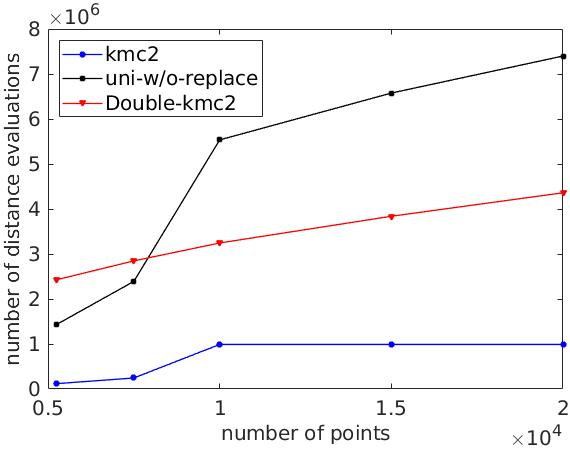
\includegraphics[width=0.44\linewidth]{syn-running-time.jpg}}
    \subfloat[]{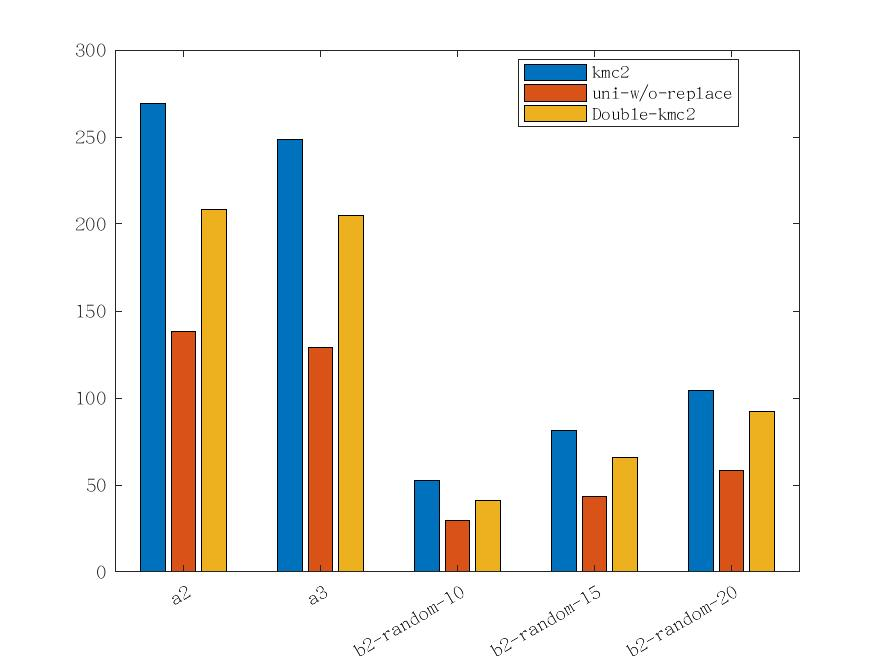
\includegraphics[width=0.44\linewidth]{syn-sum-squared-distances.jpg}} \\
    \subfloat[]{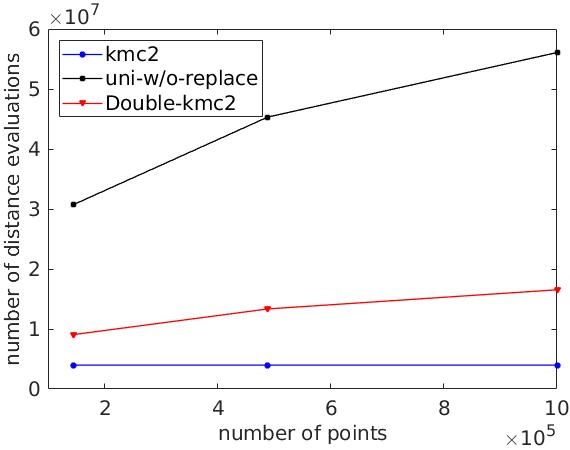
\includegraphics[width=0.44\linewidth]{real-running-time.jpg}}
    \subfloat[]{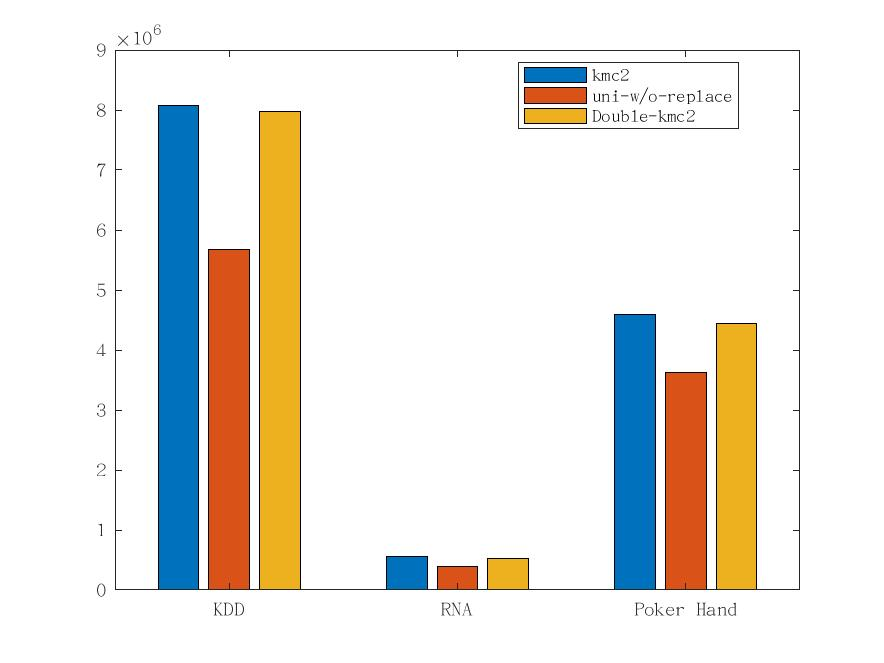
\includegraphics[width=0.44\linewidth]{real-sum-squared-distances.jpg}}
    \caption{传统聚类任务的结果。(a)合成数据集上的距离计算次数;(b)合成数据集上的$k$-means目标函数值;(c)真实数据集上的距离计算次数;(d)真实数据集上的$k$-means目标函数值}
    \label{fig: kmeans-experiments}
\end{figure}
结果见图\ref{fig: kmeans-experiments},在三个算法中基于均匀不放回采样的算法有最好的聚类效果而它的时间开销也最大,差不多是K-M$\text{C}^2$时间开销的10倍,不过随着数据量的增加,时间增加缓慢。基于均匀不放回采样的算法的$k$-means目标函数值差不多是K-M$\text{C}^2$的60\%。有意思的是,Double-K-M$\text{C}^2$的结果说明,通过K-M$\text{C}^2$采样一部分点,相比于单纯K-M$\text{C}^2$,我们能获得更好的聚类质量,而Double-K-M$\text{C}^2$的时间花费比均匀不放回要小很多。这说明,如果你倾向于一个好的聚类质量且时间开销也不想太大的话,一个好的选择是Double-K-M$\text{C}^2$,如果追求聚类质量就使用均匀不放回采样。受到特征数目和类数目的影响,$k$-means目标函数值不会随着数据量的增大而增大。图\ref{fig: kmeans-experiments}中的数据列在表\ref{tab:results on synthetic data}中,表中真实数据集上$k$-means目标函数值的数量级是$10^6$,合成数据集和真实数据集的时间开销分别在$10^6$和$10^7$数量级。

\begin{table}[h]
	\caption{传统聚类任务上$k$-means目标函数值和距离计算次数(在括号中)}
	\label{tab:results on synthetic data}
	\begin{tabular}{cccc}
		\toprule
		数据集 & K-M$\text{C}^2$ & Double-K-M$\text{C}^2$ & 基于均匀不放回采样的算法 \\
		\midrule
		% time 10^6 obj 10^0
		a2 & 269.331(0.119) & 208.395(2.428) & 138.449(1.434) \\
		a3 & 248.691(0.245) & 204.705(2.847) & 129.201(2.391) \\
		b2-random-10 & 52.358(0.990) & 41.002(3.245) & 29.519(5.536) \\
		b2-random-15 & 81.324(0.990) & 65.760(3.839) & 43.660(6.576) \\
		b2-random-20 & 104.458(0.990) & 92.411(4.361) & 58.267(7.400) \\
		\midrule % time 10^7 obj 10^7
		KDD & 8.078(0.398) & 7.978(0.908) & 5.680(3.076) \\
		RNA & 0.551(0.398) & 0.533(1.334) & 0.391(4.532) \\
		Poker Hand & 4.596(0.398) & 4.446(1.653) & 3.624(5.608) \\			
		\bottomrule
	\end{tabular}
\end{table}

\subsection{图像分割}
聚类的一个应用就是图像分割,这个应用要求对图像的不同的区块进行准确的、光滑的划分,这一应用给聚类算法聚类的质量提供了一个直观的展示。由于图像不同区块的边界不是线性的,所以需要修改$k$-means的目标函数($k$-means划分的边界是线性的),这里我们将三个算法扩展到他们对应的kernel版本。kernel $K$由以下方法构建,首先,用文献\cite{stella2003multiclass}的方法构建相似度矩阵$A$,接着,寻找一个离$A$最近的半正定矩阵$K$作为kernel,这里近与远用矩阵的Frobenius范数来度量,即求解
\begin{equation*}
	\begin{aligned}
		& \underset{K}{\text{min}} 
		& & \lVert K - A \rVert_F \\
		& s.t. 
		& & K \succeq 0
	\end{aligned}
\end{equation*}
$K \succeq 0$表示$K$是半正定矩阵。由于三个算法只返回$k$个点,$k$个划分是通过把所有点靠到离它最近的返回点上计算得到的。测试的图片是“kitten”、“bear”和“baby”\footnote{下载地址 \url{http://www.cs.utexas.edu/users/dml/Software/graclus.html}},这些图片由文献\cite{dhillon2004kernel}提供。我们调整了这些图片的长和宽,使得聚类的点的数目从900(30*30)到14400(120*120)。这个任务中kernel $k$-means的目标函数值作为聚类质量的评价指标,效率的评价指标和传统聚类中的一样。

% remark: weighted kernel kmeans++ for Double KMC^2?num of iterations?
基于均匀不放回采样的kernel版、kernel K-M$\text{C}^2$和kernel Double-K-M$\text{C}^2$的参数配置如下:均匀不放回的采样数$s' = 0.4*\log^4 n$,kernel $k$-means++是均匀不放回的$\alpha$近似算法,kernel K-M$\text{C}^2$和kernel Double-K-M$\text{C}^2$的游走次数都是200,kernel Double-K-M$\text{C}^2$的采样量是$s = 0.25*\log^2 n$,所有图片的$k$都设为5,所有算法重复30次取平均值。

\begin{figure}[h]
    \subfloat[]{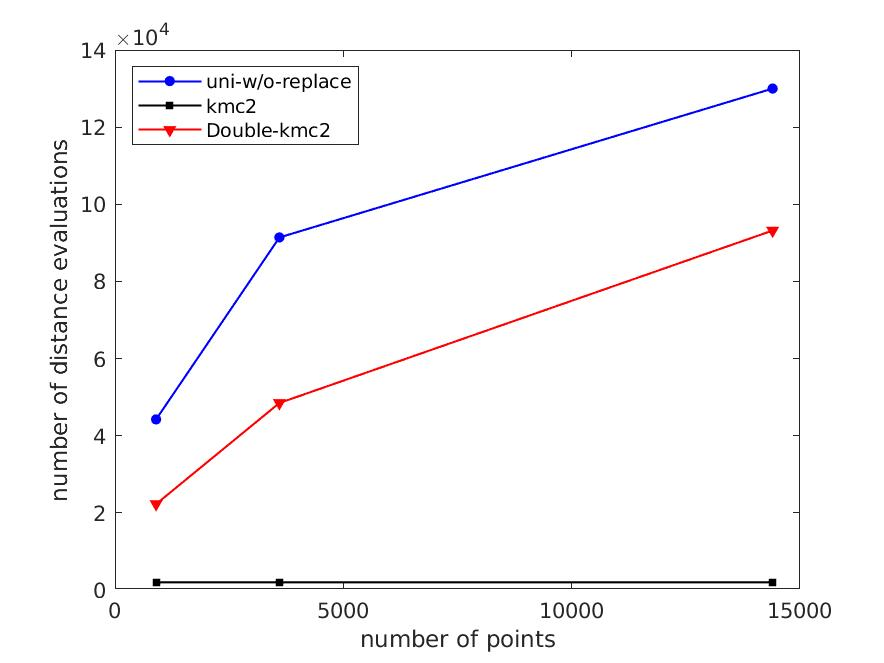
\includegraphics[width=0.44\linewidth]{image-running-time.jpg}}
    \subfloat[]{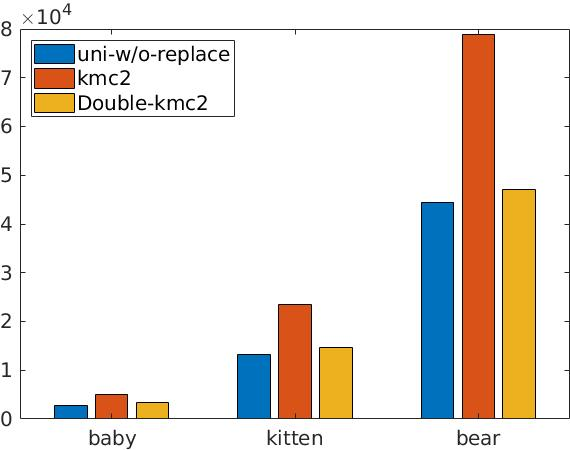
\includegraphics[width=0.44\linewidth]{image-obj.jpg}}
    \caption{图像分割任务上的结果。(a)图片数据集上的距离计算次数;(b)图片数据集上的kernel $k$-means目标函数值}
    \label{fig: image running time & ncut}
\end{figure}

% remark: 描述不量化,加上分割的图片的图,
图像分割实验结果见图\ref{fig: image running time & ncut}。实验结论和传统聚类的差不多,kernel版的均匀不放回采样有最好的聚类质量,而时间增长的趋势并不是很快,kernel Double-K-M$\text{C}^2$比均匀不放回在聚类质量上稍微差一点但是时间少了很多,kernel K-M$\text{C}^2$有最快的速度但是聚类质量太差。因此,如果你想要一个折中的平衡算法,kernel Double-K-M$\text{C}^2$是一个好的选择,如果你更关心效率,选择kernel K-M$\text{C}^2$。图\ref{fig: image running time & ncut}中的数据列在表\ref{tab:results on image segmentation}中,目标函数值的量级是$10^4$,时间开销的量级是$10^4$。
\begin{table}[h]
	\caption{图像分割任务上kernel $k$-means的目标函数值和距离计算次数(在括号中)}
	\label{tab:results on image segmentation}
	\scriptsize
	\begin{tabular}{cccc}
		\toprule
		数据集 & kernel K-M$\text{C}^2$ & kernel Double-K-M$\text{C}^2$ & 均匀不放回的kernel版 \\
		\midrule
		baby(30*30) & 0.508(0.200) & 0.341(2.228) & 0.280(4.424) \\
		kitten(60*60) & 2.345(0.200) & 1.459(4.848) & 1.323(9.140) \\
		bear(120*120) & 7.891(0.200) & 4.703(9.319) & 4.448(13.000) \\
		\bottomrule
	\end{tabular}
\end{table}

\section{本章小结}
至此,本章梳理了在$k$-means问题上的加速算法,有理论保证的算法和两者都有的算法,这些算法的相关结论总结在表\ref{tab: kmeans_algorithms}中,其中$O(\mathcal{A}_c)$是$\alpha$近似算法的时间复杂度。根据表\ref{tab: kmeans_algorithms},我们对这些算法分别从速度、理论保证和实用性这三个维度进行评价。这些算法按照时间复杂度从小到大排序如下:K-M$\text{C}^2$、均匀不放回采样(2)、AFK-M$\text{C}^2$、Lightweight Coreset、$k$-means++、算法\ref{alg: reduce_k-means2}(1)、$\epsilon$-Coreset、$k$-means++\&swap、$k$-means\(\vert \vert\) seeding、算法\ref{alg: reduce_k-means2}(2)和p-swap。在排序中,1、2名是次线性时间(需要假设),3、4名在$O(nd)$量级,5、6、7名在$O(nkd)$量级,最后4名从$O(ndk^2)$逐渐增加到$O(n^3)$。这些算法中后6名有常数近似,$k$-means++是$O(\log k)$,而前4名不是要假设就是要加方差项。最后一个,算法实用与否也非常重要,从实用角度讲,这些算法可以分为3类,第一类是AFK-M$\text{C}^2$、Lightweight Coreset、$\epsilon$-Coreset、$k$-means\(\vert \vert\) seeding,这些算法并行性较好,也无需假设,非常实用;第二类是K-M$\text{C}^2$、均匀不放回采样(2)、$k$-means++、算法\ref{alg: reduce_k-means2}(1)、算法\ref{alg: reduce_k-means2}(2)、$k$-means++\&swap,这些算法不是要假设就是有强序列属性不利于并行,实用性一般;最后剩下的就是p-swap,时间复杂度高,不实用。总结来说,如果追求速度推荐使用K-M$\text{C}^2$、均匀不放回采样(2)、AFK-M$\text{C}^2$和Lightweight Coreset,如果追求聚类质量推荐使用$\epsilon$-Coreset和$k$-means\(\vert \vert\) seeding。% remark: verify argument on $\epsilon$-Coreset

{\fontsize{10}{12}\selectfont

	\begin{longtable}{llll}
		% \small \\
		\caption{理论保证及加速相关算法结果汇总}
		\label{tab: kmeans_algorithms} \\
		\toprule
		算法 & 采样量 & 时间复杂度 & 聚类质量 \\
		\midrule
		\multirow{2}{*}{$k$-means++} & \multirow{2}{*}{$k$} & \multirow{2}{*}{$O(nkd)$} & $\E[\varphi_C(\mathcal{X})] \leq 8(\ln k + 2)$\\
		& & & $\cdot \varphi_{\text{OPT}}(\mathcal{X})$ \\
		% remark: 18+\epsilon n^3 \epsilon^{-d}
		p-swap & $k$ & $O(n^3)$ & $\varphi_C(\mathcal{X}) \leq 18 \varphi_{\text{OPT}}(\mathcal{X})$ \\
		
		$k$-means++ & \multirow{2}{*}{$k$} & \multirow{2}{*}{$O(ndk^2 \log\log k)$} & \multirow{2}{*}{$\E[\varphi_C(\mathcal{X})] \in O(\varphi_{\text{OPT}}(\mathcal{X}))$}\\
		\&swap & & & \\

		$k$-means\(\vert \vert\) & \multirow{2}{*}{$O(kt)$} & \multirow{2}{*}{$O(ndkt)$} & $\E[\varphi_S(\mathcal{X})] \leq (\frac{1+\alpha}{2})^t \xi$\\
		sampling(1) & & & $+\frac{16}{1-\alpha} \varphi_{\text{OPT}}(\mathcal{X})$ \\
		
		$k$-means\(\vert \vert\) & \multirow{2}{*}{$O(lt)$} & \multirow{2}{*}{$O(ndlt)$} & $\E[\varphi_S(\mathcal{X})] \leq 2(\frac{k}{el})^t \text{Var}(\mathcal{X})$ \\
		sampling(2) & & & $+ 26\varphi_{\text{OPT}}(\mathcal{X})$\\

		$k$-means\(\vert \vert\)& \multirow{2}{*}{$O(lt)$} & $O(ndlt)+O(ndlt)$ & $\E[\varphi_C(\mathcal{X})] \leq O(\alpha)$ \\
		seeding & & $+O(\mathcal{A}_c)$ & $\cdot \varphi_{\text{OPT}}(\mathcal{X})$ \\

		\multirow{2}{*}{K-M$\text{C}^2$} & \multirow{2}{*}{$k$} & \multirow{2}{*}{$O(k^3 d \log^2 n \log k)$} & $\E[\varphi_C(\mathcal{X})] \leq O(\log k)$  \\
		& & & $\cdot \varphi_{\text{OPT}}(\mathcal{X})$ \\

		\multirow{2}{*}{AFK-M$\text{C}^2$} & \multirow{2}{*}{$k$} & \multirow{2}{*}{$O(nd)+O(\frac{1}{\epsilon}k^2 d\log \frac{k}{\epsilon})$}& $\E[\varphi_C(\mathcal{X})]\leq 8(\log k+2)$ \\
		& & & $\cdot \varphi_{\text{OPT}}(\mathcal{X}) + \epsilon\text{Var}(\mathcal{X})$ \\

		\multirow{2}{*}{$\epsilon$-Coreset} & \multirow{2}{*}{$O(\frac{k\log k}{\epsilon^2} (dk\log k+\log\frac{1}{\delta}))$} & \multirow{2}{*}{$O(ndk\log\frac{1}{\delta})$} & $\E[\varphi_C(\mathcal{X})] \leq \alpha(1+O(\epsilon))$ \\
		& & & $\cdot \varphi_{\text{OPT}}(\mathcal{X})$ \\

		Lightweight & \multirow{2}{*}{$O(\frac{dk\log k + \log(1/\delta)}{\epsilon^2})$} & \multirow{2}{*}{$O(nd)+O(\mathcal{A}_c)$} & $\E[\varphi_C(\mathcal{X})] \leq \alpha \varphi_{\text{OPT}}(\mathcal{X})$ \\
		Coreset & & & $+ \alpha O(\epsilon) \text{Var}(\mathcal{X})$\\

		均匀不放回 & \multirow{2}{*}{$s = O(\ln \left(\frac{1}{\delta}\right) \frac{\Delta^{2} \alpha^{2}}{2 \beta^{2} m^{2}})$} & \multirow{2}{*}{$O(s)+O(\mathcal{A}_c)$} & $\E[\varphi_C(\mathcal{X})] \leq (\alpha+\beta)$ \\
		采样(1) &  &  & $\cdot \varphi_{\text{OPT}}(\mathcal{X})$ \\

		均匀不放回 & \multirow{2}{*}{$s = O(\ln(\frac{1}{\delta})\frac{\alpha^2}{\beta^2}k^2\log^4 n)$} & \multirow{2}{*}{$O(k^2 \log^4 n)+O(\mathcal{A}_c)$} & $\E[\varphi_C(\mathcal{X})] \leq (\alpha+\beta)$ \\
		采样(2) &  &  & $\cdot \varphi_{\text{OPT}}(\mathcal{X})$ \\

		\multirow{2}{*}{算法\ref{alg: reduce_k-means2}(1)} & \multirow{2}{*}{$O(k)$} & $O(nkd)+O(nkd)$ & $\E[\varphi_C(\mathcal{X})] \leq O(\alpha)$ \\
		& & $+O(\mathcal{A}_c)$ & $\cdot \varphi_{\text{OPT}}(\mathcal{X})$ \\

		\multirow{2}{*}{算法\ref{alg: reduce_k-means2}(2)} & \multirow{2}{*}{$s = \Theta\left(\frac{k \log n}{\delta^{d / 2} \varepsilon^{d}} \log ^{d / 2}\left(\frac{k \log n}{\delta^{d / 2} \varepsilon^{d}}\right)\right)$} & $O(nsd)+O(nsd)$ & $\E[\varphi_C(\mathcal{X})] \leq \alpha(1+O(\epsilon))$ \\
		& & $+O(\mathcal{A}_c)$ & $\cdot \varphi_{\text{OPT}}(\mathcal{X})$ \\

		\bottomrule
	\end{longtable}

}

梳理完算法后,我们从理论上证明了基于均匀采样的算法\ref{alg: uniform_k-means}能有更好的近似系数,具体来说从$4(\alpha+\beta)$降到了$\alpha+\beta$,并且在K-M$\text{C}^2$所依赖的两个假设,假设1和2成立的情况下,均匀采样的数目可以在$O(\log^4 n)$数量级,从而在次线性时间内取得了常数近似的解。
接着实验表明,通过多采样一些点,确实可以让均匀采样比K-M$\text{C}^2$有更好的聚类质量,在传统聚类任务和图像分割任务中这一点均有体现。
最后我们指出一些可能的未来研究方向:
\begin{enumerate}[label=\arabic*)]
	\item 在次线性时间内有理论保证且无需假设的算法,比如近似系数是$O(\log n)$的等等
	\item 提出新的次线性时间算法,依靠新的易于验证的假设
	\item 探索基于距离的自适应采样的新性质,比如进一步缩小定理\ref{theo: k-means++ overseeding2}的界,比如定义$d'(x,C) = \norm{x - c_1}+\norm{x-c_2}$,$c_1$和$c_2$分别是$C$中离$x$最近的和第二近的点,根据$d'$来挑选类,增加跳转到不同最优类的概率,以改进理论界等等。
	\item 估算权重以加速算法\ref{alg: reduce_k-means2}
	\item 考察$k$-means\(\vert \vert\) sampling是否可以形成Coreset,从而改进$k$-means\(\vert \vert\) seeding的理论界。
\end{enumerate}
随着新的分析技术的发展,$k$-means问题历久弥新,新的
理论结果依然在不断出现,实用的算法层出不穷,随着大数据
时代的到来,该问题必将焕发出新的活力。

\chapter{谱聚类}
谱聚类是从图论中演化出来的算法,后来在聚类中得到了广泛的应用。它的主要思想是把所有的数据看做空间中的点,这些点之间可以用边连接起来。点和点之间的相似度以边的权重形式体现,相似度越高权重越高。通过对所有数据点组成的图进行切图,让切图后不同的子图间边权重和尽可能的低,而子图内的边权重和尽可能的高,从而达到聚类的目的。本节我们首先介绍该问题的相关背景然后在介绍相关加速算法。
\section{谱聚类引入及背景}
由于谱聚类是基于图论的,因此我们首先温习下图的概念。

\subsection{图的概念}
对于一个图$G$,我们一般用点的集合$V$和边的集合$E$来描述。即为$G(V,E)$。其中$V$即为我们数据集里面所有的点$(v_1, v_2,...v_n)$。对于$V$中的任意两个点$v_i,v_j$,我们定义$w_{ij}$为它们之间的边的权重。谱聚类切割的图是无向图,所以$w_{ij}=w_{ji}$。
        
任意$w_{ij}\geq 0$,如果两个点不相似,$w_{ij} = 0$。对于图中的任意一个点$v_i$,它的度$d_i$定义为和它相连的所有边的权重之和,即
\begin{equation}
d_i = \sum\limits_{j=1}^{n}w_{ij}
\end{equation}
利用每个点度的定义,我们可以得到一个$n\times n$的度矩阵$D$,它是一个对角矩阵,只有主对角线有值,对应第$i$行的第$i$个点的度数,定义如下:
\begin{equation}
    D =
  \begin{pmatrix}
    d_{1} & & \\
    & \ddots & \\
    & & d_{n}
  \end{pmatrix}
\end{equation}
根据所有点间的权重值,我们可以得到图的邻接矩阵$W$,因为$W$反映了两个点的相似度,我们也把$W$称为相似度矩阵。它也是一个$n\times n$的矩阵,第$i$行的第$j$个值对应权重$w_{ij}$。
除此之外,对于点集$V$的的一个子集$A \subset V$,我们定义:
\begin{align}
& |A|: = \text{子集A中点的个数} \\
& vol(A): = \sum\limits_{i \in A}d_i
\end{align}

\subsection{相似度矩阵的构建}
在上一节我们讲到了邻接矩阵$W$,它是由任意两点之间的权重值$w_{ij}$组成的矩阵。通常我们可以自己输入权重,但是在谱聚类中,我们只有数据点的定义,并没有直接给出这个邻接矩阵,那么怎么得到这个邻接矩阵呢?

基本思想是,距离较远的两个点之间的边权重值较低,而距离较近的两个点之间的边权重值较高,不过这仅仅是定性,我们需要定量的计算。一般来说,构建邻接矩阵$W$的方法有三类。$\epsilon$-邻近法,$k$邻近法和全连接法。

对于$\epsilon$-邻近法,它设置了一个距离阈值$\epsilon$,然后用欧式距离度量任意两点$x_i$和$x_j$的距离。即令$s_{ij} = ||x_i-x_j||_2^2$,  然后根据$s_{ij}$和$\epsilon$的大小关系,来定义邻接矩阵$W$
\begin{equation}
w_{ij}= \begin{cases} 0& {s_{ij} > \epsilon}\\ \epsilon& {{s_{ij} \leq \epsilon}} \end{cases}
\end{equation}
从上式可见,两点间的权重要不就是$\epsilon$,要不就是0,没有其他的信息了。距离远近度量很不精确,因此在实际应用中,我们很少使用$\epsilon$-邻近法。

第二种定义邻接矩阵$W$的方法是$k$邻近法,利用KNN算法遍历所有的样本点,取每个样本最近的$k$个点作为近邻,只有和样本距离最近的$k$个点之间的$w_{ij}>0$。但是这种方法会造成重构之后的邻接矩阵$W$非对称,我们后面的算法需要对称邻接矩阵。为了解决这种问题,一般采取下面两种方法之一,
第一种$k$邻近法是只要一个点在另一个点的$k$近邻中,则计算$w_{ij}$
\begin{equation}
w_{ij}=w_{ji}= \begin{cases} 0& {x_i \notin KNN(x_j) \;and \;x_j \notin KNN(x_i)}\\ exp(-\frac{||x_i-x_j||_2^2}{2\sigma^2})& {x_i \in KNN(x_j)\; or\; x_j \in KNN(x_i}) \end{cases}
\end{equation}
第二种$k$邻近法是必须两个点互为$k$近邻中,才计算$w_{ij}$
\begin{equation}
w_{ij}=w_{ji}= \begin{cases} 0& {x_i \notin KNN(x_j) \;or\;x_j \notin KNN(x_i)}\\ exp(-\frac{||x_i-x_j||_2^2}{2\sigma^2})& {x_i \in KNN(x_j)\; and \; x_j \in KNN(x_i}) \end{cases}
\end{equation}

第三种定义邻接矩阵$W$的方法是全连接法,相比前两种方法,第三种方法所有的点之间的权重值都大于0,因此称之为全连接法。可以选择不同的核函数来定义边权重,常用的有多项式核函数,高斯核函数和Sigmoid核函数。最常用的是高斯核函数RBF:
\begin{equation}
w_{ij}=exp(-\frac{||x_i-x_j||_2^2}{2\sigma^2})
\end{equation}
在实际的应用中,使用第三种全连接法来建立邻接矩阵是最普遍的。

\subsection{拉普拉斯矩阵}
单独把拉普拉斯矩阵(Graph Laplacians)拿出来介绍是因为后面的算法和这个矩阵的性质息息相关。它的定义很简单,拉普拉斯矩阵$L=D-W$。D即为我们第二节讲的度矩阵,它是一个对角矩阵。而$W$即为我们第二节讲的邻接矩阵,它可以由我们第三节的方法构建出。

拉普拉斯矩阵有一些很好的性质如下:
\begin{enumerate}
    \item 拉普拉斯矩阵是对称矩阵,这可以由$D$和$W$都是对称矩阵而得。
    \item 由于拉普拉斯矩阵是对称矩阵,则它的所有的特征值都是实数。
    \item 对于任意的向量$f$,我们有
    \begin{equation}
    f^TLf = \frac{1}{2}\sum\limits_{i,j=1}^{n}w_{ij}(f_i-f_j)^2
    \end{equation}
    证明如下
    \begin{equation}
    f^TLf = f^TDf - f^TWf = \sum\limits_{i=1}^{n}d_if_i^2 - \sum\limits_{i,j=1}^{n}w_{ij}f_if_j
    \end{equation}
    \begin{equation}
    =\frac{1}{2}( \sum\limits_{i=1}^{n}d_if_i^2 - 2 \sum\limits_{i,j=1}^{n}w_{ij}f_if_j + \sum\limits_{j=1}^{n}d_jf_j^2) = \frac{1}{2}\sum\limits_{i,j=1}^{n}w_{ij}(f_i-f_j)^2
    \end{equation}
    \item 拉普拉斯矩阵是半正定的,且对应的n个实数特征值都大于等于0,即$0 =\lambda_1 \leq \lambda_2 \leq... \leq \lambda_n$, 且最小的特征值为0,这个由性质3很容易得出。
\end{enumerate}

\subsection{图切割}
        
对于无向图G的切图,我们的目标是将图$G(V,E)$切成相互没有连接的k个子图,每个子图点的集合为:$A_1,A_2,..A_k$,它们满足$A_i \cap A_j = \emptyset$,且$A_1 \cup A_2 \cup ... \cup A_k = V$.

对于任意两个子图点的集合$A, B \subset V$,我们定义A和B之间的链接为:
\begin{equation}
\operatorname{linkage}(A, B) = \sum\limits_{i \in A, j \in B}w_{ij}
\end{equation}
那么对于我们k个子图点的集合:$A_1,A_2,..A_k$,我们定义切图cut为:
\begin{equation}
cut(A_1,A_2,...A_k) = \sum\limits_{i=1}^{k}\operatorname{linkage}(A_i, \overline{A}_i )
\end{equation}
其中$\bar{A_i}$为$A_i$的补集,意为$V - A_i$。

那么如何切图可以让子图内的点权重和高,子图间的点权重和低呢?一个自然的想法就是最小化$cut(A_1,A_2,...A_k)$, 但是可以发现,这种极小化的切图存在问题,如图1所示,
\begin{figure}[h]
    \centering
    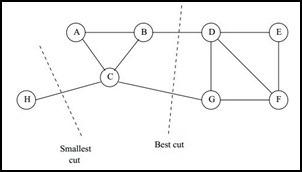
\includegraphics[scale=0.7]{cut_problem.jpg}
    \caption{可能出现的不好的切割}
\end{figure}
我们选择一个权重最小的边缘的点,比如$C$和$H$之间进行切割,这样可以最小化$cut(A_1,A_2,...A_k)$, 但是却不是最优的切图,如何避免这种切图,并且找到类似图中"Best Cut"这样的最优切图呢?我们下一节就来看看谱聚类中常用的切图方法。

\subsection{Normalized Cut}
为了避免最小切图导致的切图效果不佳,我们需要对每个子图的规模做出限定,一般来说,有两种切图方式,第一种是RatioCut,第二种是Ncut。一般我们使用Ncut,故在此只介绍Ncut\citing{shi2000normalized}。

Normalized cut切图为了避免上一节中的不好的切图,对每个切图,不光考虑最小化$cut(A_1,A_2,...A_k)$,它还同时考虑每个类中点的数目尽可能平衡,即
\begin{equation}
Ncut(A_1,A_2,...A_k) = \sum\limits_{i=1}^{k}\frac{\operatorname{linkage}(A_i, \overline{A}_i )}{vol(A_i)}
\end{equation}
为了优化该目标函数,我们定义如下指示向量。
\begin{equation}
\label{eq: spectral indicator}
h_{ij}= \begin{cases} 0& { v_i \notin A_j}\\ \frac{1}{\sqrt{vol(A_j)}}& { v_i \in A_j} \end{cases}
\end{equation}
则
对于$h_i^TLh_i$,有:
\begin{align} h_i^TLh_i & = \frac{1}{2}\sum\limits_{m=1}\sum\limits_{n=1}w_{mn}(h_{im}-h_{in})^2 \\& =\frac{1}{2}(\sum\limits_{m \in A_i, n \notin A_i}w_{mn}(\frac{1}{\sqrt{vol(A_i)}} - 0)^2 +  \sum\limits_{m \notin A_i, n \in A_i}w_{mn}(0 - \frac{1}{\sqrt{vol(A_i)}} )^2\\& = \frac{1}{2}(\sum\limits_{m \in A_i, n \notin A_i}w_{mn}\frac{1}{vol(A_i)} +  \sum\limits_{m \notin A_i, n \in A_i}w_{mn}\frac{1}{vol(A_i)})\\& = \frac{1}{2}(\operatorname{linkage}(A_i, \overline{A}_i) \frac{1}{vol(A_i)} + \operatorname{linkage}(\overline{A}_i, A_i) \frac{1}{vol(A_i)}) \\& =  \frac{\operatorname{linkage}(A_i, \overline{A}_i)}{vol(A_i)} 
\end{align}
也就是说
\begin{equation}
Ncut(A_1,A_2,...A_k) = \sum\limits_{i=1}^{k}h_i^TLh_i = \sum\limits_{i=1}^{k}(H^TLH)_{ii} = tr(H^TLH)
\end{equation}
我们将Ncut的优化问题转化为了一个二次型优化问题,并注意到该问题有如下限制
\begin{equation}
h_i^TDh_i = \sum\limits_{j=1}^{n}h_{ij}^2d_j =\frac{1}{vol(A_i)}\sum\limits_{j \in A_i}d_j= \frac{1}{vol(A_i)}vol(A_i) =1
\end{equation}
此时,我们得到如下优化问题
\begin{equation}
\label{eq: ori_spectral_clustering}
\argmin\limits_{H \in \R^{n \times k}} \; tr(H^TLH) \;\; s.t.\;H^TDH=I \quad \text{and H as in Eq. \ref{eq: spectral indicator} }
\end{equation}
注意到$H$是离散的,此时该问题是NP难的,为了求解我们允许$H$可以取连续值,该步骤称为relaxation,relax后的问题如下
\begin{equation}
    \label{eq: relax_spectral_clustering}
    \argmin\limits_{H \in \R^{n \times k}} \; tr(H^TLH) \;\; s.t.\;H^TDH=I
\end{equation}
该问题使用拉格朗日乘子法可以求解,解为$D^{-1/2}LD^{-1/2}$的最小的前$k$个特征值,对应的$H$为$D^{-1/2}LD^{-1/2}$的前$k$个特征向量,对$H$的每一行再做聚类,比如$k$-means即可得到最后的聚类结果。除了这里的relaxation外,文献\cite{bie2006fast,bresson2013multiclass,rangapuram2014tight,rangapuram2016graph}分别提出了不同的relaxation方法,不过这里的方法理论上更简单且容易实现所以非常实用,另外,文献\cite{von2007tutorial}对谱聚类给出了一份更细致的教程,感兴趣的读者可以参考,最后我们可以用一个图示来总结谱聚类的过程,见图\ref{fig: SC_illustration},可以看到谱分解相当于变换了特征,从而能够处理$k$-means处理不了的非线性可分数据。
\begin{figure}
    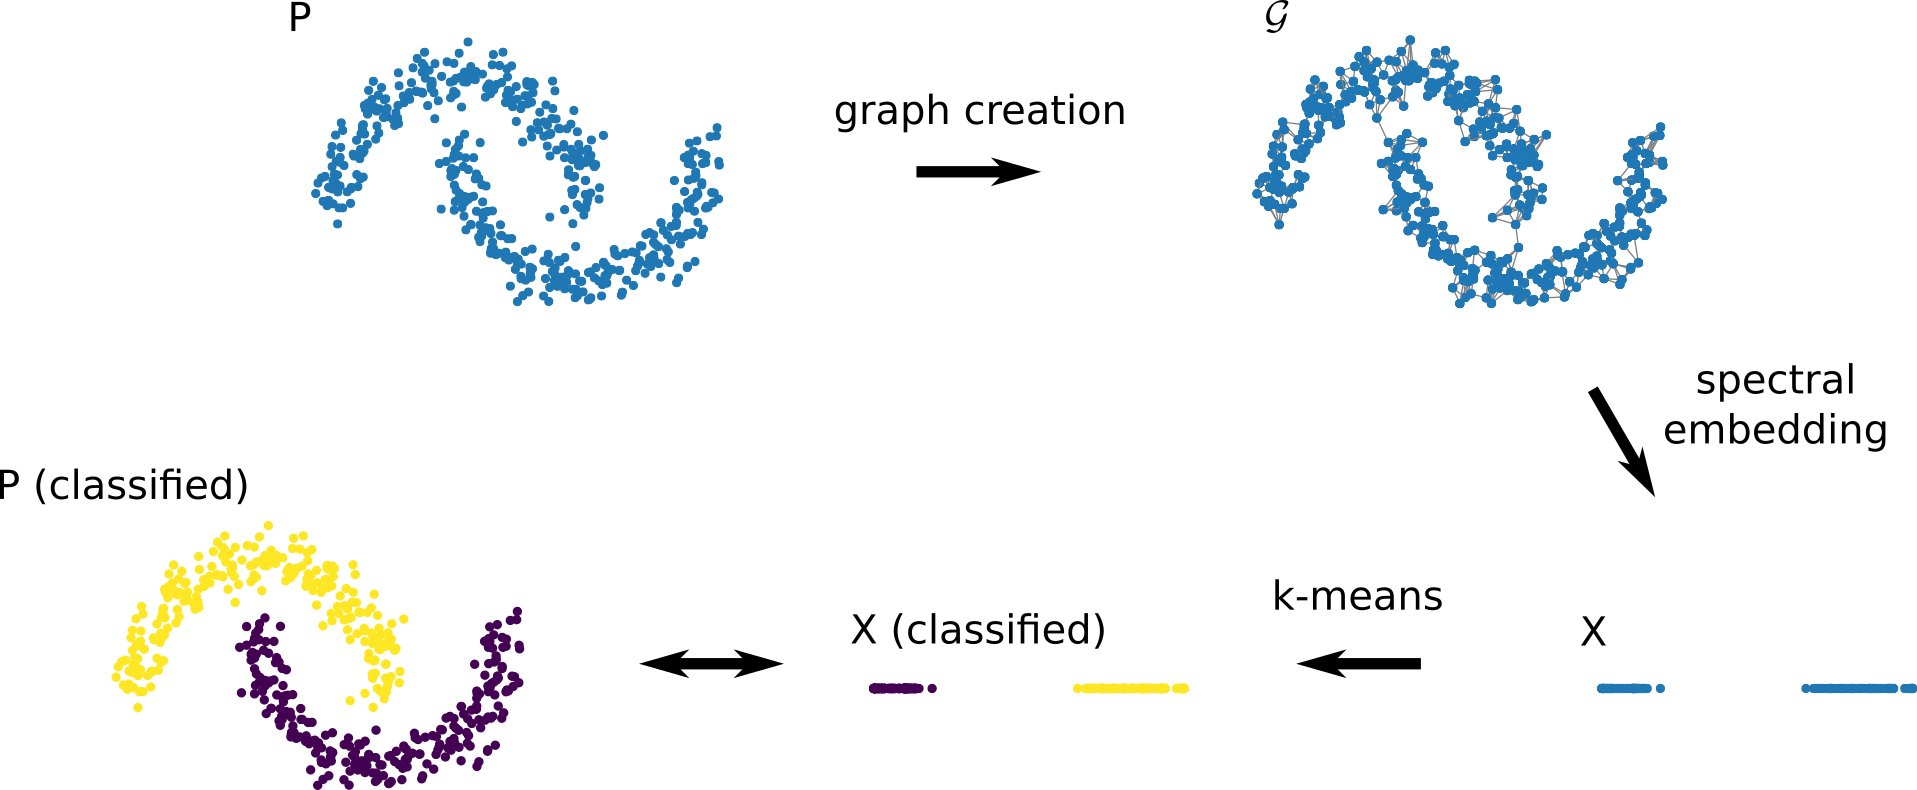
\includegraphics[width=0.8\linewidth]{SC_illustration.png}
    \caption{谱聚类过程图示}
    \label{fig: SC_illustration}
\end{figure}
\section{加速谱聚类}
谱聚类虽然效果好,能够解决$k$-means不能解决的非线性可分情况,但是其谱分解过程传统方法需要$O(n^3)$的时间复杂度,这对于大数据来说是不能够忍受的,本节,我们将从低秩近似相似度矩阵、减少数据量、低秩构建相似度矩阵三方面加速谱分解。
\subsection{低秩近似相似度矩阵}
Nyström 方法是一种半正定矩阵近似方法,可以有效近似半正定矩阵,该方法由文献\cite{williams2001using}引入到机器学习领域。其核心思想是:通过在原矩阵中采样部分列或者行,用这部分信息对原矩阵进行低秩近似。它也可以近似特征值和特征向量,通过分解大矩阵中小的子矩阵来近似大矩阵的特征值和特征向量,方法详解如下。
假设我们有一个半正定矩阵$K \in \R^{n \times n}$,因为它是半正定,所以有
\begin{equation*}
    K = X^T X
\end{equation*}
可将$X$分块,$X=[R\quad S]$,$X \in \R^{d\times n}$,其中$R \in \R^{d\times m}$,所以
\begin{align*}
    K & = \begin{bmatrix}
            R^T R & R^T S \\
            S^T R & S^T S 
          \end{bmatrix} 
\end{align*}
另一方面,我们也可以通过某种采样方法(比如均匀采样)选择$K$的$m$行(或者列),一般来说$K$表示的是数据点之间的关系,所以可以调整选中行或者列在$K$中的顺序而不会影响原始信息,不妨将选中的行调整到$K$的前排,没被选中的都放到后排,从而将$K$分块表示为如下形式
\begin{align*}
    K & = \begin{bmatrix}
            A & B \\
            B^T & C
          \end{bmatrix} 
\end{align*}
其中$[A \quad B]$是我们采样的行,此时,我们令$A = R^T R$,$B = R^T S$(通常情况,等式不会自然成立,这里我们令他们成立,目的是用$A,B$来表示$C$)。首先,我们对$A$做谱分解求得$R$,
\begin{equation*}
    A = R^T R = U\Sigma U^T
\end{equation*}
即,$R = \Sigma^{\frac{1}{2}}U^T$,又因为
\begin{equation*}
    B = R^T S = U\Sigma^{\frac{1}{2}}S
\end{equation*}
所以,$S = \Sigma^{-\frac{1}{2}}U^T B$,
此时$C \approx B^T A^{-1} B$,记用$A,B$近似的$K$为$\hat{K}$,容易知道它是$K$的一个低秩近似,秩最多是$m$,将$B^T A^{-1} B$带入$\hat{K}$有
\begin{align*}
    \hat{K} & = \begin{bmatrix}
            A & B \\
            B^T & B^T A^{-1} B
          \end{bmatrix} 
          = \begin{bmatrix}
              U\Sigma U^T & B \\
            B^T & B^T U \Sigma^{-1} U^T B
          \end{bmatrix}
          = \begin{bmatrix}
            U \\
            B^T U \Sigma^{-1}
          \end{bmatrix} \Sigma
          \begin{bmatrix}
            U^T & \Sigma^{-1}U^T B
          \end{bmatrix}
          = K_{:1}A^{-1}K_{:1}^T
\end{align*}
也就是说,我们可以用$\begin{bmatrix} U \\ B^T U \Sigma^{-1} \end{bmatrix} = K_{:1}U\Sigma^{-1}$来近似$K$的特征向量,用$A$的特征值$\Sigma$来近似$K$的特征值,这里$K_{:1} = [A \quad B]^T$是我们采样的行。由于只需要对$A$这个$\R^{m\times m}$的矩阵做分解就可以近似大矩阵的特征值和特征向量,故我们加速了大矩阵的分解。完整Nyström算法见\ref{alg: Nyström method},该算法时间复杂度是$O(nm^2 + m^3)$。
\begin{algorithm}
    \caption{Nyström 方法}\label{alg: Nyström method}
    \KwIn{半正定矩阵$K$,采样数目$m$}
    \KwOut{低秩矩阵$\hat{K}$}
    $S \gets$ 根据某些采样算法得到的列(或者行)的下标 \\
    $A \gets K(S,S)$ \\
    $K_{:1} \gets K(:,S)$ \\
    令$A = U\Sigma U^T$是$A$的谱分解,$U,\Sigma$分别是$A$的特征向量和特征值。\\
    \textbf{返回} 低秩矩阵$\hat{K} = K_{:1}A^{-1}K_{:1}^T$或者近似的特征向量$\hat{U}_K = K_{:1}U\Sigma^{-1}$
\end{algorithm} 
% 那求出$R$和$S$和加速特征值分解有什么关系呢?注意到我们实际要得到的特征向量可以从$X$处轻松获得,而要获得$X$,我们只需要对$A$这个$\R^{m\times m}$的矩阵做分解就可以获得,故我们加速了大矩阵的分解。
对于Nyström 方法,我们应该注意什么呢?第一,矩阵$K$应该本身就是低秩的,否则使用Nyström 方法将没有意义。第二,行的选择很关键,如果我们选到了大量的线性相关的行,则估计误差就会很大。
\begin{theorem}
    \label{theo: nystrom_uniform}
    令$\epsilon \in (0,1)$,$\delta \in (0,1)$,考虑用均匀采样$m$列(可以放回也可以不放回),则当$m$满足$m \geq 2 \epsilon^{-2} \mu k \log (k / \delta)$时
    \begin{equation*}
        \|K-\hat{K}\|_{2} \leq\left(1+\frac{n}{(1-\varepsilon) m}\right)\left\|K-K_{k}\right\|_{2}
    \end{equation*}
    以至少$1-3\delta$的概率成立,$\norm{.}_2$是矩阵的谱范数(spectral norm),其中
    \begin{equation*}
        \mu=\frac{n}{k} \max _{i=1, \ldots, n}\left\|V_{k}(i,:)\right\|_{2}^{2}
    \end{equation*}
    记$V$是将$K$的特征值从大到小排序后对应的特征向量,$V_{k}$是$V$的前$k$列,$K_k$是$K$的最优的秩为$k$的近似矩阵。
\end{theorem}
常用的的采样(列选择)是均匀采样,基于文献\cite{gittens2016revisiting}的结论,定理\ref{theo: nystrom_uniform}给出了均匀采样的话Nyström方法的误差,这里$\mu$被称为$V_k$的coherence。可以看到如果coherence比较大的话,均匀采样效果不太好。因此,一些更加高级的采样方法被提了出来,比如以概率$\left\|V_{k}(i,:)\right\|_{2}^{2}/k$采样第$i$列,有放回的重复$m$次的采样方式,这个概率也被称为leverage score。
\begin{theorem}
    令$\epsilon \in (0,1)$,$\delta \in (0,1)$,考虑按照上面描述的高级采样方式采样$m$列,则当$m \geq O\left(\epsilon^{-2} k \log (k / \delta)\right)$时有
    \begin{equation*}
        \|K-\hat{K}\|_{2} \leq\left\|K-K_{k}\right\|_{2}+\epsilon^{2}\left\|K-K_{k}\right\|_{*}
    \end{equation*}
    以至少$0.8-2\delta$的概率成立,其中$\norm{.}_{*}$是矩阵的迹范数(trace norm)
\end{theorem}
当然,精确计算leverage score需要对$K$做SVD,而这正是我们想避免的。尽管如此,如果$K$有$O(e)$个非零元素的话,可以在差不多$O(ek \log e)$的时间复杂度下对leverage score做近似,这里近似的误差是一个乘性误差。
到目前为止最快的利用leverage score的Nyström方法的时间复杂度接近$n$的线性函数,该算法用了一种复杂的递归的采样方式\citing{musco2017recursive}。

那么怎么将Nyström方法用到谱聚类上呢?令$A \in \R^{n \times n}$是谱聚类的相似度矩阵,它对应的归一化的拉普拉斯矩阵是$L_n = I - D^{-1/2}AD^{-1/2}$,回忆求解谱聚类需要找到$L_n$的最小的$k$个特征值对应的特征向量,这等价于找到$M = D^{-1/2}AD^{-1/2}$最大的$k$个特征值对应的特征向量,所以我们的目的就是要近似这些特征向量,通过前面的分析,我们可以通过对$A$分块拿到$A$的近似特征向量,这里的基本思想是用$A$的分块来表示$M$的分块,然后用$M$的分块利用Nyström方法近似$M$的特征向量,该方法由文献\cite{fowlkes2004spectral}提出,详解如下。我们将$A$做如下分块
\begin{equation*}
    A = \left[\begin{array}{c|c}
        A_{11} & A_{21}^T \\
      \hline
      A_{21} & A_{22}
    \end{array}\right]
\end{equation*}
我们知道的是$A_{11}$和$A_{21}$,根据Nyström方法我们可以得到一个低秩近似$\hat{A}$,根据$\hat{A}$可以得到一个近似的度矩阵$\hat{D} = \text{diag}(\hat{A}\mathbf{1})$,$\text{diag}(v)$是一个以向量$v$为对角元的对角矩阵,$\mathbf{1}$是一个元素全为1的向量,类比于$A$的分块,将$\hat{D}$分块。
\begin{equation*}
    \hat{A} = \left[\begin{array}{c|c}
        A_{11} & A_{21}^T \\
      \hline
      A_{21} & A_{21}A_{11}^{-1}A_{21}^T
    \end{array}\right],
    \hat{D} = \left[\begin{array}{c|c}
        D_{11} &  \\
      \hline
      & \hat{D}_{22}
    \end{array}\right]
\end{equation*}
有了$\hat{A}$和$\hat{D}$可以近似$M$,令近似矩阵是$\hat{M}$,则有
\begin{equation*}
    \hat{M} = \hat{D}^{-1/2}\hat{A}\hat{D}^{-1/2} = \left[\begin{array}{c|c}
        M_{11} & \hat{M}_{21}^T \\
      \hline
      \hat{M}_{21} & \hat{M}_{22}
    \end{array}\right]
\end{equation*}
其中$M_{11} = D_{11}^{-1/2}A_{11}D_{11}^{-1/2}$,$\hat{M}_{21} = \hat{D}_{22}A_{21}D_{11}^{-1/2}$,记$\hat{M}_{:1} = \begin{bmatrix}
    M_{11} \\
    \hat{M}_{21}
\end{bmatrix}$,此时即可用算法\ref{alg: Nyström method}来近似$M$的特征向量,只不过此时算法\ref{alg: Nyström method}中的$A$是$M_{11}$,$K_{:1}$是$\hat{M}_{:1}$。

值得注意的是,这样求出来的的近似特征向量不可直接基于它用$k$-means聚类,原因是这个近似的特征向量列不正交,由于不正交,基于这样的特征向量可能得出的谱聚类的解质量很差,所以我们需要对现有近似特征向量做后处理,使其正交。在文献\cite{fowlkes2004spectral}中,作者根据分块矩阵$M_{11}$是否是半正定的提出了两种方法。

(一)$M_{11}$是半正定

首先,考虑将$\hat{M}$写成谱分解的样子
\begin{align*}
    \hat{M} &= \begin{bmatrix}
        M_{11} \\ \hat{M}_{21}
    \end{bmatrix} M_{11}^{-1}
    \begin{bmatrix}
        M_{11} & \hat{M}_{21}^T
    \end{bmatrix} \\
    &= \left( \begin{bmatrix}
        M_{11} \\ \hat{M}_{21}
    \end{bmatrix} M_{11}^{-1/2} U \Sigma^{-1/2} \right) \Sigma \left( \Sigma^{-1/2} U^T M_{11}^{-1/2} \begin{bmatrix}
        M_{11} & \hat{M}_{21}^T \end{bmatrix} \right) \\
    &= V\Sigma V^T
\end{align*}
上式中$\Sigma$是任意对角矩阵,$U$是任意正交矩阵,为了求出$U$和$\Sigma$,我们要求$V$列正交,有
\begin{align*}
    I &= V^T V \\
    &= \left( \Sigma^{-1/2} U^T M_{11}^{-1/2} \begin{bmatrix}
        M_{11} & \hat{M}_{21}^T \end{bmatrix} \right) \left( \begin{bmatrix}
        M_{11} \\ \hat{M}_{21} \end{bmatrix} M_{11}^{-1/2} U \Sigma^{-1/2} \right) \\
\end{align*}
对上面等式左乘$U \Sigma^{1/2}$,右乘$\Sigma^{1/2} U^T$,有
\begin{align*}
    U\Sigma U^T &= \left( M_{11}^{-1/2} \begin{bmatrix}
        M_{11} & \hat{M}_{21}^T \end{bmatrix} \right) \left( \begin{bmatrix}
        M_{11} \\ \hat{M}_{21} \end{bmatrix} M_{11}^{-1/2} \right) \\
        &= M_{11} + M_{11}^{-1/2} \hat{M}_{21}^T \hat{M}_{21} M_{11}^{-1/2}
\end{align*}
所以说,我们只要对$S = M_{11} + M_{11}^{-1/2} \hat{M}_{21}^T \hat{M}_{21} M_{11}^{-1/2}$做谱分解,得到它的特征向量$U_S$和特征值$\Sigma_S$就可以得到$M$的近似特征向量$V = \begin{bmatrix} M_{11} \\ \hat{M}_{21} \end{bmatrix} M_{11}^{-1/2} U_S \Sigma_S^{-1/2}$

(二)$M_{11}$不是半正定

如果$M_{11}$不是半正定,$M_{11}^{-1/2}$就没有定义,前面方法就不可以正交化,文献\cite{fowlkes2004spectral}中将情况1的方式称为one-shot,因为不用求出不正交的特征向量,而这里需要按照以下两步进行。首先,根据前面的方法得出近似的但是不正交的特征向量$\bar{V} = \hat{M}_{:1}U_{M_{11}}\Sigma_{M_{11}}^{-1}$,其中$U_{M_{11}}$和$\Sigma_{M_{11}}^{-1}$分别是$M_{11}$的特征向量和特征值。接着,取$Z = \bar{V}\Sigma_{M_{11}}^{1/2}$,这样$\hat{M} = ZZ^T$,对$Z$做奇异值分解,$U_Z$即为所求的正交化处理后的特征向量
\begin{equation*}
    Z = U_{Z}\Sigma_{Z}V_Z^T
\end{equation*}

这个基于Nyström方法加速谱聚类的方法总结见算法\ref{alg: Nyström spectral},这里$\hat{U}_{:k}$是$\hat{U}$最大的$k$个特征值对应的特征向量。该算法的时间复杂度是$O(nm^2+m^3)$,如果$m$比较大,时间开销还是会比较大,文献\cite{li2011time,choromanska2013fast}对此做了进一步改进。
% remark: 调整算法的输入,让算法更清楚,写算法的时间复杂度
\begin{algorithm}[h]
    \caption{Nyström 方法加速谱聚类}\label{alg: Nyström spectral}
    \KwIn{近似的相似度矩阵$\hat{A}$}
    \KwOut{归一化拉普拉斯矩阵$L_n$最小的$k$个特征值对应的特征向量}
    $\hat{D} \gets \text{diag}(\hat{A}\mathbf{1})$\\
    $M_{11} \gets D_{11}^{-1/2}A_{11}D_{11}^{-1/2}$ \\
    $\hat{M}_{21} \gets \hat{D}_{22}A_{21}D_{11}^{-1/2}$ \\
    \uIf{$M_{11}$是半正定矩阵}{
        $S = M_{11} + M_{11}^{-1/2} \hat{M}_{21}^T \hat{M}_{21} M_{11}^{-1/2}$ \\
        $U_S,\Sigma_S \gets $ 对$S$做谱分解得到它的特征向量和特征值 \\
        $\hat{U} = \begin{bmatrix} M_{11} \\ \hat{M}_{21} \end{bmatrix} M_{11}^{-1/2} U_S \Sigma_S^{-1/2}$
    }
    \Else{
        $U_{M_{11}},\Sigma_{M_{11}} \gets $ 对$M_{11}$做谱分解得到它的特征向量和特征值 \\
        $Z \gets \begin{bmatrix} M_{11} \\ \hat{M}_{21} \end{bmatrix} U_{M_{11}} \Sigma_{M_{11}}^{-1/2}$ \\
        $\hat{U} \gets $ 对$Z$做奇异值分解得到它的左奇异矩阵
    }
    \textbf{返回} $\hat{U}_{:k}$
\end{algorithm}

\subsection{减少数据量}
类似于$k$-means问题,谱聚类中一种自然的加速方法也是减少数据量,这个想法的框架如下:
\begin{enumerate}
    \item 采样$m$个数据点,将这些点称为采样集
    \item 在采样集上运行谱聚类算法
    \item 再将剩下的点靠到已有的解上得到全部数据点的划分
\end{enumerate}
这个框架下一个经典的算法是KASP\citing{yan2009fast},算法描述见算法\ref{alg: KASP},
算法时间复杂度是$O(nmdt+m^3)$,其中$t$是Lloyd的迭代次数。那么,这个算法的近似误差是多少呢?这里,我们对文献\cite{yan2009fast}的分析做一个简单的总结。在算法\ref{alg: KASP}中$x_i$到$y_j$的关系是通过$k$-means建立的,这个$x_i$到$y_j$的关系也可以看做是$x_i$经过扰动得到的$y_j$,即$x_i+\epsilon_i = y_j$,这里$\epsilon_i$是数据点的扰动,所以这里的$k$-means可以看做一种将$\mathcal{X}$扰动到$Y$的过程,扰动后的结果是$$\mathcal{X}' = \{y_1,...,y_1,y_2,...,y_2,...,y_k,...,y_k\}$$,令$y_i$的重复次数是$r_i$,则$\sum_{i=1}^k r_i = n$。一般的,我们令扰动后的结果是$\tilde{\mathcal{X}} = \{x_1+\epsilon_1,...,x_n+\epsilon_n\}$,考虑基于$\mathcal{X}$和$\tilde{\mathcal{X}}$的谱聚类结果的区别$\rho$,定义$$\rho=\frac{1}{n} \sum_{i=1}^{n} \mathbb{I}\left\{I_{i} \neq \tilde{I}_{i}\right\}$$,$\mathbb{I}$是指示函数,内里表达式如果为真就是1,$I = (I_1,...,I_n)$,$I_i$表示了点$x_i$的类id,$\tilde{I} = (\tilde{I}_1,...,\tilde{I}_n)$,$\tilde{I}_i$表示了点$\tilde{x}_i$的类id。基于文献\cite{huang2009spectral}的工作,可得如下定理。
\begin{theorem}[KASP的理论保证]
    在文献\cite{yan2009fast}中定理3假设条件成立情况下,有$\rho \leq O\left(\frac{k}{g_{0}^{2}}\|L-\tilde{L}\|_{F}\right)$,其中$g_0$是一个依赖谱间距(spectral gap)的值,$L$和$\tilde{L}$分别对应$\mathcal{X}$和$\tilde{\mathcal{X}}$的拉普拉斯矩阵。同时,如果文献\cite{yan2009fast}中定理6假设成立,则下式会以一个大概率成立
    \begin{equation*}
        \|L-\tilde{L}\|_{F} \leq O\left(\sigma_{\epsilon}^{(2)}+\sigma_{\epsilon}^{(4)}\right)
    \end{equation*}
    其中$\sigma_{\epsilon}^{(2)}$和$\sigma_{\epsilon}^{(4)}$是扰动项$\epsilon$的范数$\norm{\epsilon}$的二阶和四阶矩。
\end{theorem}
由上面两个理论界,$\rho$就可以被$\norm{\epsilon}$的二阶和四阶矩限定住,而Lloyd算法实际是在最小化二阶矩,从这一点来讲,用$k$-means得到采样集的过程有理论支持。除去Lloyd算法得到采样集,还有一个算法叫eSPEC也可以用来得到采样集,详见文献\cite{wang2009approximate}。
\begin{algorithm}
    \caption{KASP}\label{alg: KASP}
    \KwIn{数据集$\mathcal{X} = \{x_1,x_2,...,x_n\}$,类数目$k$,采样数目$m$}
    \KwOut{$\mathcal{X}$的$k$个划分}
    在$\mathcal{X}$上运行Lloyd算法,令$k=m$,得到中心点$Y = \{y_1,y_2,...,y_m\}$\\
    对$\mathcal{X}$和$Y$建立关联字典,$x_i:y_j$(key:value),其中$y_j$是离$x_i$最近的$Y$中的点 \\
    在$Y$上做一个谱聚类,类数目是$k$ \\
    对任意$x_i$,根据$\mathcal{X}$和$Y$的关联字典查找$y_j$,再根据$y_j$的类id,得到$x_i$的类id\\
    \textbf{返回}$\mathcal{X}$的$k$个划分
\end{algorithm}

\subsection{低秩构建相似度矩阵}
除去上述的两种方法,还有一种基于landmark/anchor的方法\citing{liu2010large,cai2014large},landamark/anchor其实也是一些采样点,不过这里采样是为构建相似度矩阵做准备,这类方法思路如下。

首先,通过Lloyd或者一些其他的采样方法得到一个采样集$W \in \R^{d \times m}$,$m$是采样数,下一步是把这$m$个点当做一组基,用这组基去表示$n$个点使得$\mathcal{X} \approx WB$,这里$B \in \R^{n \times m}$即是根据基得到的表示矩阵。有了$B$,我们就可以用$B$去构建相似度矩阵$A$,$$A = B\Delta^{-1}B$$ 这里$\Delta$是一个对角矩阵,其中$\Delta_{jj} = \sum_{i=1}^n B_{ij}$,这个对角阵起一个归一化的作用。这里用$BB^T$表示$A$的一个直觉是,如果两个点的$m$维表示比较接近的话,这两个点的相似度应该比较高,那么反过来可以用他们的内积来表示他们的相似度。这个相似度矩阵$A$的一个好处是,可以令$P = B\Delta^{-1/2}$,从而让$A = PP^T$,这样就可通过对$P$做奇异值分解得到$A$的特征向量,从而让分解的时间复杂度降到$O(nm^2)$。一种构建$B$的方法是求解下式\citing{chen2017scalable,nie2016constrained}。$$\min _{B_i \mathbf{1}=1, B_i \geq 0} \sum_{j=1}^{m} B_{i j}\left\|\mathbf{x}_{i}-\mathbf{w}_{j}\right\|_{2}^{2}+\gamma \sum_{j=1}^{m} B_{i j}^{2}$$ 这里$B_i$是$B$的第$i$行。

综上,我们总结了三种基于采样的加速谱分解的方法,他们的共同点是都基于采样,但是各个方法的采样目的不同。对Nyström方法来说,采样是为了低秩近似相似度矩阵,而低秩近似带来的一个副产品是可以近似特征向量,这个方法是不用知道相似度矩阵是怎么构建的的,假设采样$m$个点,只需要计算$n \times m$的相似度矩阵,分解$m \times m$的那一部分就可以得到近似的特征向量,另一方面Nyström方法有很好的理论支撑,基于Nyström方法的大都有清晰的理论结果,Nyström方法的延伸也很广,可以广泛用在矩阵近似上,比如kernel近似等\citing{wang2014efficient,wang2014modified,sun2015review}。对KASP来说,采样是为了减少数据,分解的是一个$m \times m$的矩阵,缺点是得不到近似的特征向量,因此方法的扩展性不是很好。对基于landmark/anchor的方法来说,采样的目的是得到一个相似度矩阵,采样的副产品是这个相似度矩阵由于构建方法的关系可较为方便计算特征向量,这个方法的缺点也很明显,这个方法得到的特征向量和相似度构建方式紧密绑定,如果相似度矩阵是别人给的或者某种其他规定的方式生成的的话,这个方式是没有办法用的,另外,这个方法分解的时间复杂度也比前两种方法高。

由于都是采样方法,采样方式是很关键的,如果采样的列或者数据点线性相关性比较强的话,对于Nyström方法来说近似的矩阵的秩和真实的就会差很多,对基于landmark的方法来说$WB$的秩就会比真实数据小很多,从而损失很多信息。对于Nyström方法来说,除去均匀采样和利用leverage score的方法以外,还有很多其他的采样方式,文献\cite{kumar2012sampling}是一个好的总结。对于基于landmark/anchor的方法来说,常用的生成landmark的方法除了Lloyd还有比如BKHK\citing{zhu2017fast}、BKM\citing{chen2018spectral}等。最后,除了这里提到的三种采样方式外,最近的文献\cite{tremblay2020approximating}还提到了很多其他的方式并给出了有洞见的观点,是很好的参考资料。

% 都是采样,但是目的不同
% 其他anchor方法
% 不同方法缺点
% 共同点
\section{改进谱聚类聚类质量}
本节我们探究如何改进谱聚类的质量,我们从两个维度考虑,一个方面是谱分解后的聚类质量来提高谱聚类的质量,另一方面是,通过把谱聚类转换成带权kernel $k$-means问题,用前述的$k$-means的一些方法来给谱聚类提供理论保证。

\subsection{改进谱分解后的聚类}
谱分解后,$k$个$n$维的特征向量使得每个数据点变为了一个$k$维向量,这个过程也可以理解为每个数据点经过特征变换获得了新的特征,这些新的特征有时也会称为谱嵌入(spectral embedding),在传统的谱聚类中通过Lloyd算法将谱嵌入转化为离散的划分,但是Lloyd算法终究不够准确,这里我们考虑一些方法来改进这一转换的过程。文献\cite{stella2003multiclass}提出了一种后来被称为谱旋转\citing{huang2013spectral,chen2017scalable}的方法。回忆谱聚类的过程,原问题是式\ref{eq: ori_spectral_clustering},文献\cite{stella2003multiclass}对式\ref{eq: ori_spectral_clustering}做如下等价改写,
\begin{equation*}
	\max _{Y \in I n d, Z=Y\left(Y^{T} D_{A} Y\right)^{-\frac{1}{2}}} \operatorname{Tr}\left(Z^{T} A Z\right)
\end{equation*}
这里$Y \in B^{n \times k}$是0/1标记矩阵(目的是解出它),值只能取0/1,每一行只有一个1,$A$是相似度矩阵,$D_A$是$A$的度矩阵,对上式relax后得到下式
\begin{equation*}
	\max _{Z^{T} D_{A} Z=I_{k}} \operatorname{Tr}\left(Z^{T} A Z\right)
\end{equation*}
其中$I_k$是$k\times k$的单位阵,这个relaxation和式\ref{eq: relax_spectral_clustering}是等价的,这个问题的最优解$Z^*$是$D_A^{-1}A$最大的$k$个特征向量。注意到,如果对$Z^*$右乘正交矩阵,上面relax式目标值不会改变,换句话说,我们可以用$Z^*R$去逼近$Z$,这里的$R$是一个正交矩阵,这便是谱旋转。在文献\cite{stella2003multiclass}中,在求得$Z^*$后,作者对$Z^*$的每一行做了行归一化(每一行的行范数是1),得到$Y^*$。然后再用$Y^*R$去逼近$Y$,
\begin{equation*}
 	\min_{Y \in I n d,R^TR = RR^T = I_k} \norm{Y - Y^*R}_F^2
\end{equation*}
为什么要归一化呢?可能是作者觉得原来的$Y$每一行范数也是1,为了把relax后的解变回到原来的$Y$的空间,需要做行归一化。但是,注意到$Z$和$Y$的关系,$Z=Y\left(Y^{T} D_{A} Y\right)^{-\frac{1}{2}}$,也即是说$Y$是做了列的伸缩得到的$Z$,那么行的归一化就不是一种合理的操作。文献\cite{chen2017scalable}显然注意到了这一点,提出另一种更合理的谱旋转,核心思想是不把$Z^*$变为$Y^*$,直接让用$Z^*R$去逼近$Z$,从而得到下式
\begin{equation*}
	\min_{Y \in I n d,R^TR = RR^T = I_k} \norm{Y\left(Y^{T} D_{A} Y\right)^{-\frac{1}{2}} - Z^*R}_F^2
\end{equation*}
对上式的求解得到了更好的聚类质量,那么为什么谱旋转会比Lloyd更适合呢?文献\cite{huang2013spectral}对这一点给出了说明。给定谱嵌入$Q \in \R^{n \times k},$如果用Lloyd求解,我们可以得到如下的矩阵表示
\begin{equation*}
	\min_{G \in Ind,H\in \R^{k \times k}} \norm{Q - GH}_F^2
\end{equation*}
如果用谱旋转便是
\begin{equation*}
	\min_{G \in Ind,R^TR=RR^T=I_k} \norm{G-QR}_F^2
\end{equation*}
根据酉不变性和正交矩阵对称阵也是正交矩阵可知,上式可以写作
\begin{equation*}
	\min_{G \in Ind,R^TR=RR^T=I_k} \norm{Q-GR}_F^2
\end{equation*}
经过对比,我们容易发现,之所以谱旋转比解$k$-means更好是因为对$H$施加了正交限制,缩小了$H$的范围自然更容易得到更好的$G$。

\subsection{带权kernel \texorpdfstring{$k$}{k}-means问题}
这个方法的基本思想是将谱聚类问题转为$k$-means问题,这样上一章所提出的各种有理论保证的算法就可以在谱聚类上。我们先介绍带权kernel $k$-means问题,再介绍这两者应该如何建立等价性。
\begin{definition}[带权kernel $k$-means问题]
    \label{def: weighted_kernel_kmeans}
    给定集合 $\mathcal{X} \subseteq \R^d$ 和每一个$x \in \mathcal{X}$ 的权重 $w_i$, 找到一个大小为$k$的集合 $C$ 使得下述目标函数能最小
    \begin{equation*}
        \Psi(\mathcal{X},C) = \sum_{i=1}^k \sum_{x_j \in \pi_i}w_j \norm{\phi(x_j)-C_i}^2
    \end{equation*}
    这里$\pi_i$是第$i$个类,$\cup_{i=1}^k \pi_i = \mathcal{X}$,$\phi(.)$表示映射函数,$C_i = \frac{\sum_{x_j \in \pi_i}w_j \phi(x_j)}{\sum_{j \in \pi_i}w_j}$。
\end{definition}
根据$K_{ij} = \phi(x_i)^T\phi(x_j)$,和上式$C_i$的定义,我们可以如下计算高维中点$\phi(a_i)$到一个中心点$m_c$的距离,
\begin{equation*}
	\norm{\phi(a_i) - m_c}^2 = K_{i i}-\frac{2 \sum_{a_{j} \in \pi_{c}} w_{j} K_{i j}}{\sum_{a_{j} \in \pi_{c}} w_{j}}+\frac{\sum_{a_{j}, a_{l} \in \pi_{c}} w_{j} w_{l} K_{j l}}{\left(\sum_{a_{j} \in \pi_{c}} w_{j}\right)^{2}}
\end{equation*}
由此,我们得到一个求解带权kernel $k$-means问题的算法,带权kernel Lloyd算法\citing{dhillon2004unified},见算法\ref{alg: weighted_kernel_Lloyd},该算法时间复杂度是$O(n^2 \tau)$,$\tau$是迭代次数。
\begin{algorithm}
    \caption{带权kernel Lloyd算法}\label{alg: weighted_kernel_Lloyd}
    \KwIn{数据集$\mathcal{X}$,类数目$k$,kernel $K$,权重$w$,最大迭代次数$t_{\text{max}}$}
    \KwOut{$\mathcal{X}$的$k$个划分}
    随机将$\mathcal{X}$划分,记划分为$\pi$,当前的迭代次数为$t$,初始值0\\
    \While{$t<t_{\text{max}}$}{
    	对每个数据点$a_i$和类$c$的中心点$m_c$计算距离
	    \begin{equation*}
	    	d(a_i,m_c) \gets K_{i i}-\frac{2 \sum_{a_{j} \in \pi_{c}} w_{j} K_{i j}}{\sum_{a_{j} \in \pi_{c}} w_{j}}+\frac{\sum_{a_{j}, a_{l} \in \pi_{c}} w_{j} w_{l} K_{j l}}{\left(\sum_{a_{j} \in \pi_{c}} w_{j}\right)^{2}}
	    \end{equation*}\\
	    更新每个点对应的所属类,记点$a_i$更新后的类id是$C_i^* = \argmin\limits_{c = 1,2,...,k} d(a_i,m_c)$,则$\pi_c$更新后的划分是
	    \begin{equation*}
	    	\pi_c = \{a_i|C_i^*=c\}
	    \end{equation*}\\
	    $t\gets t+1$
    }
    \textbf{返回}$\mathcal{X}$的$k$个划分
\end{algorithm}
根据文献\cite{dhillon2004unified},带权重kernel $k$-means问题的目标函数值$\Psi(\mathcal{X},C)$可以写成矩阵形式
\begin{equation*}
	% \label{eq: matrix_form_wkk}
	\Psi(\mathcal{X},C) = \operatorname{Tr}\left(W^{1 / 2} K W^{1 / 2}\right)-\operatorname{Tr}\left(\tilde{Y}^{T} W^{1 / 2} K W^{1 / 2} \tilde{Y}\right)
\end{equation*}
其中$\tilde{Y} = W^{1/2}X(X^TWX)^{-1/2}$,这里$X\in B^{n\times k}$是上一小节的0/1划分矩阵,接下来,我们揭示谱聚类同上面介绍的带权kernel $k$-means问题的联系。回忆谱聚类是最小化Ncut,这也等价于最大化Nassoc,这里
\begin{equation*}
	Nassoc=\sum_{i=1}^k \frac{\operatorname{linkage}(A_i,A_i)}{vol(A_i)} = \operatorname{Tr}(\tilde{Y}^TD^{-1/2}AD^{-1/2}\tilde{Y})
\end{equation*}
其中$\tilde{Y} = D^{1/2}X(X^TDX)^{-1/2}$,这里我们取$W=D,K=D^{-1}AD^{-1}$,并注意到$Ncut+Nassoc=k$即可得到下式
\begin{equation}
	\label{eq: wkk_spectral_clustering}
	\Psi(\mathcal{X},C) = \operatorname{Tr}\left(D^{-1 / 2} A D^{-1 / 2}\right) - k + Ncut
\end{equation}
其中等式右边的前两项是一个和划分无关的常数,上式说明,只要令$W=D,K=D^{-1}AD^{-1}$,求解带权kernel $k$-means问题就是在解决谱聚类!通过前面的推导,我们知道带权$k$-means++是一个$O(\log k)$近似的算法,显然在kernel下依然有$O(\log k)$的近似,所以我们可以用$k$-means++或者其他的有理论保证的$k$-means算法使得谱聚类也有理论保证!不仅如此,这一等式还说明我们可以绕过谱分解从而减少大量时间。

除去上面的两种方法外还有其他的改进谱聚类聚类质量的方法,比如在relax的时候施加更紧的限制\cite{yang2018new},直接求解谱聚类的离散问题\cite{chen2018spectral}等等。

% 可以做的方向:coreset 谱聚类
% \section{加速谱聚类且有理论保证}
\section{基于均匀采样算法的新理论结果}
既然可以把谱聚类转换成带权kernel $k$-means问题,那么前一章的算法\ref{alg: uniform_k-means}是不是可以扩展到谱聚类上呢?答案是显然的,扩展后的算法如下,
\begin{algorithm}
    \caption{基于均匀不放回采样的带权kernel $k$-means算法(直觉)}
    \KwIn{映射后的数据集$\phi(\mathcal{X})$,类数目$k$,采样数$s$}
    \KwOut{$\phi(\mathcal{X})$的$k$个划分}
    $S \gets$ 从$\phi(\mathcal{X})$中均匀采样$s$个点\\
    $C \gets$ 在带权$S$上运行一个$\alpha$近似算法\\
    把$\phi(\mathcal{X})$靠到离自己最近的$C$上,得到数据点的$k$个划分\\
    \textbf{返回}$\phi(\mathcal{X})$的$k$个划分
\end{algorithm}
但是这样的算法没有办法实现,因为一般情况下我们拿不到点经过映射后的新特征,有的$\phi$会把点映射到无穷维,我们能参与运算的只有kernel,所以真正的算法见算法\ref{alg: uniform_wkk},这里$W(S,S)$和$K(S,S)$是基于采样索引获得的$W$和$K$的子矩阵,$Y\in B^{n\times k}$,该算法时间复杂度是$O(s^2+ns)$(如果$D$是单位阵的话)。类似定理\ref{theo: uniform_k-means},文献\cite{Mohan:2017:BNA:3172077.3172235}得出了带权kernel $k$-means下的对应定理。
\begin{theorem}[均匀不放回采样的谱聚类解的质量]
    \label{theo: uniform_wkk}
    令 $0 < \delta <1/2$, $\alpha \geq 1$, $\beta >0$是近似的参数。令$C$是由算法\ref{alg: uniform_wkk}中$\pi$所对应的中心点. 假设我们均匀不放回的采样$s$个点,如果,
    \begin{equation*}
    s \geq \ln(\frac{1}{\delta})(1+\frac{1}{n})/(\frac{\beta^2 m^2}{2\Delta^2 \alpha^2}+\frac{\ln(1/\delta)}{n})
    \end{equation*}
    则,我们有
    \begin{equation*}
    Ncut \leq 4(\alpha + \beta) Ncut^* + 4(\alpha + \beta)c
    \end{equation*}
    以至少 $1-2\delta$的概率, 其中$\Delta = \max\limits_{i,j}\norm{\phi(x_i) - \phi(x_j)}^2$是高维下数据直径的平方, $m = \Psi(\mathcal{X},C_{\text{OPT}_k}^{\mathcal{X}})/n$是点到其对应的中心点的距离的平均值,$c$是一个划分无关的常数,$Ncut^*$是最优的Ncut。
\end{theorem}
\begin{algorithm}
	\SetNoFillComment
    \caption{基于均匀采样和带权kernel $k$-means的谱聚类算法}\label{alg: uniform_wkk}
    \KwIn{数据集$\mathcal{X}$,类数目$k$,采样数$s$,相似度矩阵$A$,度矩阵$D$}
    \KwOut{$\mathcal{X}$的$k$个划分}
    $S \gets$ 从$1,2,...,n$中均匀采样$s$个数字\\
    $W \gets D,K \gets D^{-1}AD^{-1}$\\
    $W_s \gets W(S,S), K_s \gets K(S,S)$\\
    $\pi \gets$ 基于$W_s$和$K_s$,在带权$S$上运行一个$\alpha$近似算法\\
    \tcc{把点靠到高维中由采样点得到的中心点上}
    \For{$i = 1,...,n$}{
    	\For{$c = 1,...,k$}{
    		\begin{equation*}
	    	d(a_i,m_c) \gets K_{i i}-\frac{2 \sum_{a_{j} \in \pi_{c}} w_{j} K_{i j}}{\sum_{a_{j} \in \pi_{c}} w_{j}}+\frac{\sum_{a_{j}, a_{l} \in \pi_{c}} w_{j} w_{l} K_{j l}}{\left(\sum_{a_{j} \in \pi_{c}} w_{j}\right)^{2}}
	    	\end{equation*}\\
    	}
    	$j \gets \argmin\limits_{c = 1,2,...,k} d(a_i,m_c)$\\
    	$Y_{ij} \gets 1$
    }
    \textbf{返回}$Y$
\end{algorithm}
类似前面我们的更紧理论界,定理\ref{theo: uniform_k-means_sharper},这里也可以把定理\ref{theo: uniform_wkk}做的更紧,从而得出下面的定理。
\begin{theorem}[均匀不放回采样的谱聚类解的质量]
    \label{theo: uniform_wkk_sharper}
    令 $0 < \delta <1/2$, $\alpha \geq 1$, $\beta >0$是近似的参数。令$C$是由算法\ref{alg: uniform_wkk}中$\pi$所对应的中心点. 假设我们均匀不放回的采样$s$个点,如果,
    \begin{equation*}
    s \geq \ln(\frac{1}{\delta})(1+\frac{1}{n})/(\frac{\beta^2 m^2}{2\Delta^2 \alpha^2}+\frac{\ln(1/\delta)}{n})
    \end{equation*}
    则,我们有
    \begin{equation*}
    Ncut \leq (\alpha + \beta) Ncut^* + (\alpha + \beta)c
    \end{equation*}
    以至少 $1-2\delta$的概率, 其中$\Delta = \max\limits_{i,j}\norm{\phi(x_i) - \phi(x_j)}^2$是高维下数据直径的平方, $m = \Psi(\mathcal{X},C_{\text{OPT}_k}^{\mathcal{X}})/n$是点到其对应的中心点的距离的平均值,$c$是一个划分无关的常数,$Ncut^*$是最优的Ncut。
\end{theorem}
由于证明和前面$k$-means的很相似,这里不再详细展开,唯一需要注意的是在得到$\Psi(\mathcal{X},C) \leq (\alpha+\beta) \Psi(\mathcal{X},C_{\text{OPT}_k}^{\mathcal{X}})$后,将式\ref{eq: wkk_spectral_clustering}带入即可完成证明。
\section{实验}
在上一节,我们证明了基于均匀采样的算法在谱聚类上有更紧的理论界,另一方面,算法\ref{alg: uniform_wkk}能把谱聚类$O(n^3)$的时间复杂度降到$O(s^2+ns)$。在本节,我们就实现这一算法,用实验来体现该算法在实践中可以又快又好的解决谱聚类问题。这里,我们在6个数据集\footnote{下载地址 \url{http://www.escience.cn/people/chenxiaojun/index.html}}上做实验,数据集描述见表\ref{tab:datasets_spectral_clustering}。
\begin{table}[h]
	\caption{数据量$n$, 类数目$k$, 维度$d$}
	\label{tab:datasets_spectral_clustering}
	\begin{tabular}{ccccc}
		\toprule
		数据集 & 名字 & $n$ & $d$ & $k$ \\
		\midrule
		$D_1$ & segment &2310 & 19 & 7 \\
		$D_2$ & MnistData-05 &3495 &784 & 10 \\
		$D_3$ & MnistData-10 &6996 & 784 & 10 \\
		$D_4$ & isolet5 &7797 & 617 & 26 \\
		$D_5$ & USPS &9298 & 256 & 10 \\
		$D_6$ & letter-recognition &20000 & 16 & 26 \\
		\bottomrule
	\end{tabular}
\end{table}

参与实验的算法是算法\ref{alg: uniform_wkk},其中$\alpha$近似算法是带权kernel $k$-means++,实验基准算法是带权kernel $k$-means++后接带权kernel Lloyd(即算法\ref{alg: uniform_wkk}不采样的版本)。实验中相似度矩阵$A$的构建方式采用了文献\cite{chen2017scalable}的方法,anchor数目是数据点数目的20\%,算法\ref{alg: uniform_wkk}的采样数目也是数据点数目的20\%,两个算法的最大迭代次数都是30。由于随机性,算法\ref{alg: uniform_wkk}和基准算法在每个数据集上都会重复20次,取平均值汇报。Ncut和时间(秒)分别用来评价谱聚类聚类质量和聚类速度。

\begin{figure}[h]
    \subfloat[]{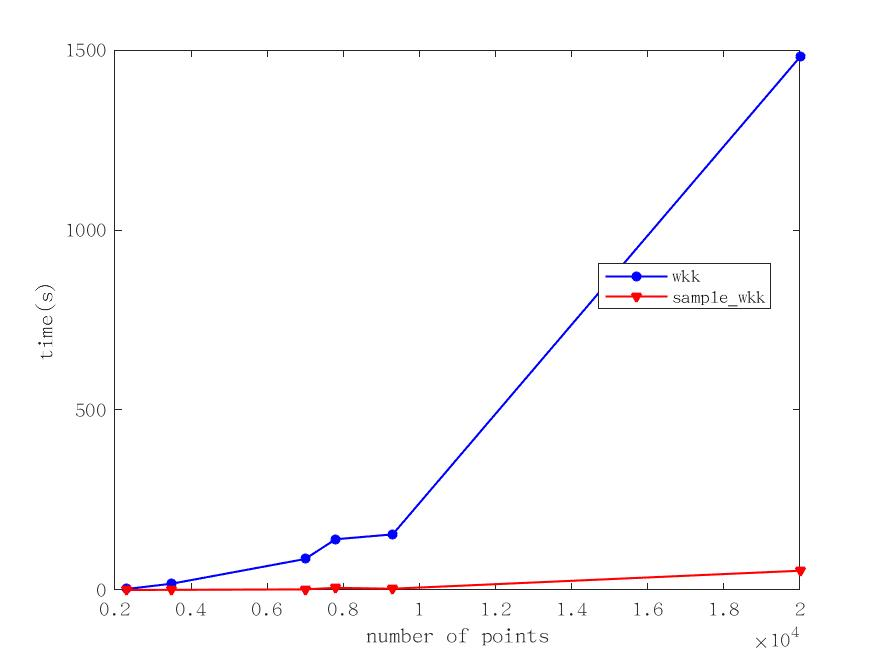
\includegraphics[width=0.45\linewidth]{sp-running_time.jpg}}
    \subfloat[]{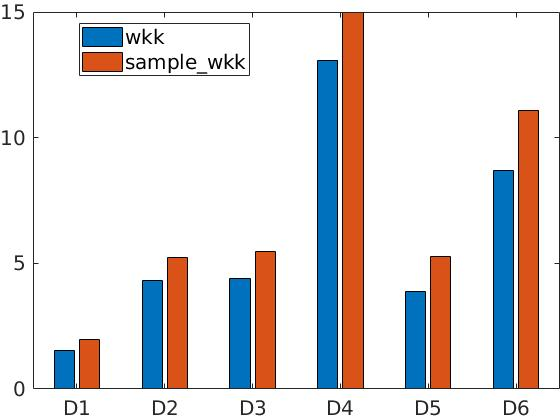
\includegraphics[width=0.45\linewidth]{sp-Ncuts.jpg}}
    \caption{谱聚类结果。(a)聚类所花时间(秒);(b)谱聚类的Ncut;}
    \label{fig: sp-experiments}
\end{figure}
结果见图\ref{fig: sp-experiments},从图中我们可以看出,基于采样的方法解决谱聚类的速度比不采样快了20~50倍,非常显著的加速了谱聚类的求解,另一方面,基于采样的方法的聚类质量又没有比不采样差太多,Ncut比不采样大了0.5~2.4,平均下来不超过不采样的25\%,较不采样而言,采样对聚类质量的影响不太显著,这验证了算法\ref{alg: uniform_wkk}在实践中可以又快又好的解决谱聚类问题。图\ref{fig: sp-experiments}中的数据列在表\ref{tab: res_spectral_cls}中。
\begin{table}[h]
	\caption{谱聚类Ncut和时间(时间在括号中,单位:秒)}
	\label{tab: res_spectral_cls}
	\begin{tabular}{ccc}
		\toprule
		数据集 & 带权kernel $k$-means & 采样的带权kernel $k$-means \\
		\midrule
		$D_1$ & 1.52(2.8) & 1.97(0.1) \\
		$D_2$ & 4.31(17.6) & 5.24(0.4) \\
		$D_3$ & 4.40(86.2) & 5.47(1.7) \\
		$D_4$ & 13.09(140.9) & 14.97(6) \\
		$D_5$ & 3.86(154.5) & 5.25(3.5) \\
		$D_6$ & 8.69(1480.6) & 11.10(53.6) \\
		\bottomrule
	\end{tabular}
\end{table}


\section{本章小结}
本章我们先介绍了图论的背景,引入拉普拉斯矩阵,从图切割的角度引入了谱聚类。由于谱聚类需要做谱分解,而大规模数据下谱分解是非常耗时的,我们随后从三个方向上介绍了谱聚类的加速,第一个方法使用Nyström方法,这一方法是一种常用的矩阵低秩近似技术,它的副产品是加速特征向量的计算,通过低秩近似的相似度矩阵,得到了近似的拉普拉斯矩阵的特征向量,第二个方法是减少数据量,通过在一些采样集上做谱聚类从而得到所有点的划分,其中用Lloyd算法获得采样集的方式有理论上的道理,最后一个方法依然是用采样,不过采样的目的是构建低秩的相似度矩阵,这一矩阵的副产品是特征向量容易计算。然后,我们介绍了如何改进谱聚类的聚类质量,一种方法是改进谱分解后的聚类,算法是谱旋转,这一算法是贴合谱聚类的目标函数设计的,另一种方法是将谱分解同带权kernel $k$-means建立联系,用上一章所述的有理论保证的算法即可让谱聚类有理论保证。当然,也可直接用上一章的$k$-means算法替换这里谱分解后的Lloyd算法,这里不再赘述。接着,我们给出了基于采样的方法可以又快又好的完成谱聚类,并证明了这一方法可以有更紧的理论保证。在随后的实验环节中,我们在实验上验证了这一算法的有效性和高效性。

最后,我们指出一些谱聚类未来的可能研究方向:
\begin{enumerate}[label=\arabic*)]
	\item 作为谱聚类的核心,相似度矩阵的设计是一个开放性问题,不好的设计会让聚类结果和人的预期有较大出入。
	\item 用Coreset的思想加速谱聚类,使得谱聚类可以获得更好的理论结果。
	\item 解决均匀采样的一些问题,目前采样数和直径挂钩,所以采样数可能很大,另外,由于$K = D^{-1}AD^{-1}$,尽管只需要计算$n \times s$的kernel,但是需要完整计算相似度矩阵$A$,传统方法时间复杂度是$O(n^2)$,所以我们需要对这一步加速,并得出相应的理论结果。
\end{enumerate}
谱聚类作为非线性聚类的经典算法,早年被频繁的用在图像分割中,得益于其优秀的聚类效果,随着大数据时代的到来,新的分析技术和实用的算法必将给这一问题带来新的活力。
\chapter{全文总结与展望}

\section{全文总结}
本文研究了大数据下扁平聚类的两个问题,分别是如何加速聚类以及如何获得更好的解的。第一章,我们引入了聚类的概念,建立了聚类的工作流,简单介绍了常用的聚类算法,随后指出了本文的研究目标和行文结构。在本文中,我们具体研究了$k$-means问题和谱聚类问题,第二章,在$k$-means问题中,我们介绍了基于$k$-means++和局部搜索的方法来改进Lloyd算法的聚类质量,用各种采样方法(均匀不放回、Coreset)来减少数据量从而加速了$k$-means的求解,我们将采样和理论保证的方法拼在一起让$k$-means可以又快又好的被解决。接着,我们给出了我们的贡献,首先,$k$-means++算法被扩展到了带权重的$k$-means问题上,我们证明了这一扩展后的方法可以取得$O(\log k)$的近似,其次,我们证明了基于均匀不放回采样方法可以有更紧的$k$-means理论界,同时,在温和的数据假设下,均匀采样的数目可以被限定在$O(\log^4 n)$,从而让$k$-means可以在多项式对数时间复杂度下获得常数近似的解,在本章的最后,通过和K-M$\text{C}^2$以及新提出的Double-K-M$\text{C}^2$做实验上的对比从而实践中验证了基于均匀采样的方法可以加速$k$-means的求解且获得有保证的聚类质量。

然后,在第三章中,我们探索了谱聚类问题,谱聚类能够解决$k$-means不能解决的非线性划分的问题,在实践中效果好。然而,这一算法需要谱分解,用常规的分解方法需要$O(n^3)$的时间复杂度,所以我们首先介绍了如何加速谱聚类。加速的方法分为三种,第一种是用Nyström方法低秩近似,这一方法的副产物是近似的特征向量,由于只需要分解采样的小矩阵,时间复杂度大大减少,第二种方法是减少数据量,这一方法更为直接,即在采样点上聚类,然后利用数据点和采样点的关系得到所有点的聚类,最后一种方法利用采样构建相似度矩阵,这一矩阵本身就是低秩的,分解的是$n\times m$的矩阵,时间复杂度从$O(n^3)$降到了$O(nm^2)$,$m$是采样数。随后,我们指出了改进谱聚类的方法,一种是用谱旋转改进谱分解后的聚类,另一种方法是将谱聚类问题转换为带权kernel $k$-means问题,再用前述的理论保证算法给谱聚类提供保证。随后,我们给出了本文在谱聚类上的贡献,将均匀不放回方法扩展到带权kernel $k$-means上,证明了谱聚类的更紧的理论界,随后,在实验环节,我们在实践中确认了通过均匀采样,谱聚类速度可以很快,同时聚类质量又不会损失很多。

\section{后续工作展望}
在提出$k$-means问题和Lloyd算法的50、60年后,聚类依然在蓬勃发展。考虑到连贯性,在2、3章的最后,我们分别给出了一些可能的$k$-means和谱聚类的未来可能方向,这里我们站在一个更高的角度,尝试回答对于聚类来说,未来的研究方向和可能的重要的未解决问题,我们认为有以下问题值得探索。

聚类算法的选择。在这个问题上,传统的理论派和实践派都忽视了,理论派往往关心如何加速聚类,如何证明更好的理论结果等等,而对于实践派来说,聚类算法的选择往往过于随意,比如速度快、程序开源、算法好懂等,但是这些选择方式忽略了本质,即,我们应该根据实践中问题的需要选择算法。对于聚类来说,需求可能会有很多,比如相似的点要在一个类,不相似的在不同的类,不同的类的大小要平衡,不能有的类很大,有的类很小等。需要注意的是,这些要求往往不能同时满足,比如文献\cite{ben2018clustering}指出相似的点要在一个类,不相似的在不同的类这两个要求有的时候会互相冲突,所以我们需要明确在自己的任务中哪些聚类要求是主要的,并且,我们需要知道不同的算法会满足哪些需求,即算法的偏好(bias),我们应该根据这两个点来选择我们的算法,不过对于聚类算法的终端用户来说,他们不是聚类算法研究人员,他们往往很难用术语说清自己的聚类需要什么需求。所以,对于聚类算法的选择依然是一个开放性问题。

弥补实践和理论的鸿沟。对于传统的理论派来说,他们往往分析的是最差情况下的算法理论界,对于$k$-means和谱聚类这样的NP难问题,最差情况下算法的时间复杂度是指数级。但是,在现实情况中,简单的经验性算法,比如Lloyd算法一般也能取得不错的效果,另一方面,对于一个3层的中间层神经元数目超过3的神经网络来说,训练它都是NP难的问题,但是现实却是我们取得了新一轮的深度学习的辉煌,这种现实和理论脱离的感觉不免让人疑惑。这中间缺失了什么使得现实的情况比理论情况好的多?在聚类上,或许是现实的数据更加“可分”?事实上,有一些工作通过添加数据的假设说明了在这些数据上聚类是容易的,算法可以在多项式时间结束。不过,多数假设非常难验证,而且,通过仔细分析,可以发现这些假设对数据施加的限制很多是不现实的,所以对于理论派来说,未来需要提出更好的能够易于验证的假设,且需要增加自己的理论工具来放松对数据的限制从而解释现实情况,更进一步的,理论派需要在解释现实情况的基础上去指导未来算法的设计。

其他问题。这里提一些潜在的小问题,比如类数目$k$怎么选?如果$k$在一个范围内都是合适的,怎么设计聚类的目标函数?聚类的理论基石等等。

最后,随着新硬件的不断加持和理论工具的逐渐扩充,我们有理由相信未来以聚类为代表的无监督方法能够引领人工智能的前进,能够更好的处理海量数据,从而让未来人类在技术的帮助下享受美好的人生。



% misc

\thesisacknowledgement
光阴荏苒,岁月如梭,转眼七年电子科技大学的学习生涯即将画上句号。在这七年间,除了专业知识,在生活和工作上也学到了很多,这些将会是我人生中重要的财富,伴我面向未来的人生。值此论文完成之际,我首先要感谢导师xxx教授对我学习上的帮助,犹记得当初看不懂论文的数学,老师帮我联系了数学学院的老师,帮助我扫清数学障碍,看懂文章。在选题上老师也给予我充分的自由,允许我按照兴趣来做,而不把我当做廉价劳动力,在教师节老师也不鼓励我们送礼,反而请我们吃饭,老师的德行令我敬佩,在今后的工作中他将是我学习的榜样。接着,我要感谢本科和研究生的辅导员老师以及导生,六一姐、钟sir,感谢你们日常对我们的呵护以及帮我们申请和处理各项学院事宜。感谢本科和研究生阶段的同学们,有你们的陪伴学习变得不再孤独,本科后许久不见的朋友们,你们还好吗?感谢我的父母和家人,你们用行动展示了对我的爱。感谢百忙中腾出时间审阅本文的老师和教授,你们的帮助会让这篇文章变得越来越好。最后,感谢母校电子科技大学,感谢学校为我们创建了舒适的学习环境和多彩的文化生活,让我充实的度过了七年时光,希望下次回来清水河能够让校友划船。我们下一站见!


\thesisappendix

\chapter{常见的concentration bound}
在概率论中,concentration bound描述了随机变量是怎么偏离一个数的(通常是其均值),一个经典案例是大数定律。我们在这里列一些常用的,在正文的证明中也有用到相关的concentration bound。

\begin{theorem}[Markov 不等式]
	令$X$是一个非负的随机变量,则,对任意常数$a>0$,有
	\begin{equation*}
		P(X \geq a) \leq \frac{\E[X]}{a}
	\end{equation*}
\end{theorem}

\begin{theorem}[Chebyshev 不等式]
	令$X$是一个随机变量,则,对任意常数$a>0$,如果方差是有限的,有
	\begin{equation*}
		P(|X-\E[X]| \geq a) \leq \frac{\text{Var}[X]}{a^{2}}
	\end{equation*}
\end{theorem}

\begin{theorem}[Hoeffding 不等式]
	令$X_1,X_2,...,X_n$是独立的随机变量,其中$a_i \leq X_i \leq b_i$,令$c_i = b_i - a_i$,$S_n = \sum_{i=1}^n X_i$,$E_n = \E[S_n] = \sum_{i=1}^n \E[X_i]$,则有
	\begin{equation*}
		P\left[\left|S_{n}-E_{n}\right|>t\right]<2 \exp \left(-\frac{2 t^{2}}{\sum_{i=1}^{n} c_{i}^{2}}\right)
	\end{equation*}
\end{theorem}

% Uncomment to list all the entries of the database.
% \nocite{*}

\thesisbibliography{reference}

%
% Uncomment the following code to load bibliography database with native
% \bibliography command.
%
% \nocite{*}
% \bibliographystyle{thesis-uestc}
% \bibliography{reference}
%

% comment while no need
\thesisaccomplish{publications}
% \input{misc/translate_original}
% \input{misc/translate_chinese}

\end{document}
